\documentclass{article}
\usepackage[utf8]{inputenc}

\title{Empowering local IT with open-source tools}
\author{Lauri Võsandi}
\date{January 2015}

\usepackage{natbib}
\usepackage{graphicx}
\usepackage{url}
\usepackage{tikz}

\begin{document}

\maketitle

\section{Introduction}

This minor thesis complements the major thesis
titled \emph{Efficient and Reliable Filesystem Snapshot Distribution}.


\section{Background}

IT is essential infrastructure for every country, especially developing countries.
The harsh reality is that western IT corporations often offer products
and services for developing countries at non-sustainable prices in order
to gain userbase. Once the county has reached certain living standard the
pricing is adjusted accordingly.


As the users have been learning to use particular product,
reluctance to switch is increased due to training costs,
user fustration etc.
Most often organizations submit to paying licensing fees at significantly
higher prices due to users protesting against change.

Starting from the end of 2013 Microsoft does not consider Estonia a developing country
anymore. The implication of the change was that the Microsoft Windows and Microsoft
Office license fees would rise from current 6 EUR to 60 EUR per month per machine.
According to Ernst \& Young analysis Tallinn could save 490 000 EUR within 5 years
if they would give up Microsoft Office now. Replacing Windows with Linux would
save additional 210 000 EUR. This was the main motivation for Tallinn Education Department to try out alternatives. As change from Microsoft Office to LibreOffice was certain, replacing operating system was more questionable.

In March of 2014 they decided to pilot Linux in 5 educational institutions: Mustamäe Upper Secondary School [2], Tallinn Mahtra Primary School [3], Merivälja school [4], Tallinn Mesimummu kindergarten [5] and Tallinn Tammetõru kindergarten [6]. Procurement competition was won by Arvuti Traumapunkt OÜ [7] and Silver Püvi hired me to take care of setting up infrastructure servers. Most of the work so far has been done remotely in conjunction with local IT-support. Before the migration I had around 7 years of open-source hacking experience, however I never had experience with remote management or centralized authentication.

\section{Examples}

\subsection{

\subsection{Wireless networks}

With the introduction of various e-study systems the requirements for
wireless networks have increased significantly.
EstWin project started in 2009 promised to establish fibre links within 1.5km range
from each Estonian household
\footnote{\url{http://www.elasa.ee/}}.
Estonian Educational Network will be covering the last mile for each school of Estonia
by 2016.
This means by next year each Estonian school is about to have gigabit link to the premises.

In Estonia western vendors offer wireless coverage for educational institutions
at varying prices.
As organizations don't know what they need they usually get enterprise solution which
is overpriced and exceeds their requirements.

Youtube states
that for 720p video stream 2.5Mbps downlink is required.
The average sized classroom houses approximately 20-30 students.
This is yields an upper bound of 75MBps per classroom.
As 5GHz poorly penetrates concrete wall it makes sense to place
access point in each room.
It's also a good idea to provide public and protected networks
simultaneously.

To reiterate the requirements for wireless network:

\begin{itemize}

  \item{5GHz support for modern mobile devices}
  \item{2.4GHz support for legacy devices}
  \item{802.11n support for better throughput}
  \item{Roaming support}
  \item{Multi-SSID support}
  \item{Central configuration management}
  \item{WPA2 Enterprise support for eduroam}
\end{itemize}
Enterprise grade hardware which conforms to the requirements:

* Ruckus ... 500 EUR


Considering that all the mentioned vendors impose vendor lock-ins
(closed source firmware, firmware signature checks, etc)
it might not be a good idea to have the software of the hardware vendor.
For example Colubris was acquired by Hewlett Packard in 2008 and many products
sold by Colubris are unsupported and customers are left with
deprecated hardware.

In fact most wireless hardware vendors are using open-source, but
fail to adhere to General Public License conditions which should grant
the hardware user the freedom to modify the software.
Cisco \footnote{http://www.fsf.org/news/2008-12-cisco-suit}
Mikrotik \footnote{https://www.mail-archive.com/legal@lists.gpl-violations.org/msg00335.html}
and other enterprise hardware vendors are in fact taking advantage
of open-source software to build their products, but GPL license conditions
are blatantly disregarded.

After analyzing various hardware that is supported by OpenWrt
a decision was made in favour of TP-Link WDR4300.
This particular router
contains Atheros system on chip and Atheros wireless chips
which are also used in enterprise products.
Atheros wireless chips support 802.11abgn, multiple SSID-s,
RADIUS authentication and much more.

Using OpenWrt a completely binary-blob free firmware can be built.
The lack of blobs has it's merits - latest Linux kernel can be used
and all security updates are available significantly earlier.
Vendor back-doors can also be mitigated using customized firmware.


In Estonia western vendors offer wireless coverage for educational institutions
at varying prices.
As organizations don't know what they need they usually get enterprise solution which
is overpriced and exceeds their requirements.
As an example 46000 EUR price was offered to cover 7-floor building.

Using common sense, open-source tools and open-source friendly hardware
sustainable and reasonably priced solutions can be built.

802.11abgn compliant TP-Link WDR4300 can be obtained at sub 60 EUR pricetag.
Gigabit capable (802.11ac) TP-Link Archer C7 can be obtainer at around 100 EUR.
A regular PC can be used for routing purposes


\begin{figure}[!htb]
\centering
\scalebox{0.5}{% Graphic for TeX using PGF
% Title: /home/lauri/msc-thesis/dia/wlan-controller.dia
% Creator: Dia v0.97.2
% CreationDate: Wed Mar 25 16:47:18 2015
% For: lauri
% \usepackage{tikz}
% The following commands are not supported in PSTricks at present
% We define them conditionally, so when they are implemented,
% this pgf file will use them.
\ifx\du\undefined
  \newlength{\du}
\fi
\setlength{\du}{15\unitlength}
\begin{tikzpicture}
\pgftransformxscale{1.000000}
\pgftransformyscale{-1.000000}
\definecolor{dialinecolor}{rgb}{0.000000, 0.000000, 0.000000}
\pgfsetstrokecolor{dialinecolor}
\definecolor{dialinecolor}{rgb}{1.000000, 1.000000, 1.000000}
\pgfsetfillcolor{dialinecolor}
\pgfsetlinewidth{0.100000\du}
\pgfsetdash{}{0pt}
\pgfsetdash{}{0pt}
\pgfsetbuttcap
\pgfsetmiterjoin
\pgfsetlinewidth{0.040000\du}
\pgfsetbuttcap
\pgfsetmiterjoin
\pgfsetdash{}{0pt}
\definecolor{dialinecolor}{rgb}{0.000000, 0.682353, 0.850980}
\pgfsetstrokecolor{dialinecolor}
\pgfpathmoveto{\pgfpoint{32.275359\du}{3.832830\du}}
\pgfpathlineto{\pgfpoint{32.275359\du}{2.046727\du}}
\pgfusepath{stroke}
\pgfsetlinewidth{0.200000\du}
\pgfsetbuttcap
\pgfsetmiterjoin
\pgfsetdash{}{0pt}
\definecolor{dialinecolor}{rgb}{0.000000, 0.682353, 0.850980}
\pgfsetstrokecolor{dialinecolor}
\pgfpathmoveto{\pgfpoint{32.275359\du}{3.804008\du}}
\pgfpathlineto{\pgfpoint{32.275359\du}{2.578846\du}}
\pgfusepath{stroke}
\pgfsetbuttcap
\pgfsetmiterjoin
\pgfsetdash{}{0pt}
\definecolor{dialinecolor}{rgb}{0.000000, 0.000000, 0.000000}
\pgfsetfillcolor{dialinecolor}
\pgfpathmoveto{\pgfpoint{32.327217\du}{2.218350\du}}
\pgfpathlineto{\pgfpoint{32.218042\du}{2.218350\du}}
\pgfpathlineto{\pgfpoint{32.218042\du}{2.000000\du}}
\pgfpathlineto{\pgfpoint{32.327217\du}{2.000000\du}}
\pgfpathlineto{\pgfpoint{32.327217\du}{2.218350\du}}
\pgfusepath{fill}
\pgfsetlinewidth{0.100000\du}
\pgfsetbuttcap
\pgfsetmiterjoin
\pgfsetdash{}{0pt}
\definecolor{dialinecolor}{rgb}{0.000000, 0.682353, 0.850980}
\pgfsetstrokecolor{dialinecolor}
\pgfpathmoveto{\pgfpoint{32.327217\du}{2.218350\du}}
\pgfpathlineto{\pgfpoint{32.218042\du}{2.218350\du}}
\pgfpathlineto{\pgfpoint{32.218042\du}{2.000000\du}}
\pgfpathlineto{\pgfpoint{32.327217\du}{2.000000\du}}
\pgfpathlineto{\pgfpoint{32.327217\du}{2.218350\du}}
\pgfusepath{stroke}
\pgfsetlinewidth{0.040000\du}
\pgfsetbuttcap
\pgfsetmiterjoin
\pgfsetdash{}{0pt}
\definecolor{dialinecolor}{rgb}{0.000000, 0.682353, 0.850980}
\pgfsetstrokecolor{dialinecolor}
\pgfpathmoveto{\pgfpoint{29.627865\du}{3.832830\du}}
\pgfpathlineto{\pgfpoint{29.627865\du}{2.046727\du}}
\pgfusepath{stroke}
\pgfsetlinewidth{0.200000\du}
\pgfsetbuttcap
\pgfsetmiterjoin
\pgfsetdash{}{0pt}
\definecolor{dialinecolor}{rgb}{0.000000, 0.682353, 0.850980}
\pgfsetstrokecolor{dialinecolor}
\pgfpathmoveto{\pgfpoint{29.627865\du}{3.804008\du}}
\pgfpathlineto{\pgfpoint{29.627865\du}{2.578846\du}}
\pgfusepath{stroke}
\pgfsetbuttcap
\pgfsetmiterjoin
\pgfsetdash{}{0pt}
\definecolor{dialinecolor}{rgb}{0.000000, 0.000000, 0.000000}
\pgfsetfillcolor{dialinecolor}
\pgfpathmoveto{\pgfpoint{29.679724\du}{2.218350\du}}
\pgfpathlineto{\pgfpoint{29.570549\du}{2.218350\du}}
\pgfpathlineto{\pgfpoint{29.570549\du}{2.000000\du}}
\pgfpathlineto{\pgfpoint{29.679724\du}{2.000000\du}}
\pgfpathlineto{\pgfpoint{29.679724\du}{2.218350\du}}
\pgfusepath{fill}
\pgfsetlinewidth{0.100000\du}
\pgfsetbuttcap
\pgfsetmiterjoin
\pgfsetdash{}{0pt}
\definecolor{dialinecolor}{rgb}{0.000000, 0.682353, 0.850980}
\pgfsetstrokecolor{dialinecolor}
\pgfpathmoveto{\pgfpoint{29.679724\du}{2.218350\du}}
\pgfpathlineto{\pgfpoint{29.570549\du}{2.218350\du}}
\pgfpathlineto{\pgfpoint{29.570549\du}{2.000000\du}}
\pgfpathlineto{\pgfpoint{29.679724\du}{2.000000\du}}
\pgfpathlineto{\pgfpoint{29.679724\du}{2.218350\du}}
\pgfusepath{stroke}
\pgfsetbuttcap
\pgfsetmiterjoin
\pgfsetdash{}{0pt}
\definecolor{dialinecolor}{rgb}{0.000000, 0.682353, 0.850980}
\pgfsetfillcolor{dialinecolor}
\pgfpathmoveto{\pgfpoint{33.015893\du}{4.059586\du}}
\pgfpathcurveto{\pgfpoint{33.015893\du}{4.490828\du}}{\pgfpoint{32.116946\du}{4.840406\du}}{\pgfpoint{31.007947\du}{4.840406\du}}
\pgfpathcurveto{\pgfpoint{29.898947\du}{4.840406\du}}{\pgfpoint{29.000000\du}{4.490828\du}}{\pgfpoint{29.000000\du}{4.059586\du}}
\pgfpathlineto{\pgfpoint{29.000000\du}{5.203304\du}}
\pgfpathcurveto{\pgfpoint{29.000000\du}{5.634654\du}}{\pgfpoint{29.898947\du}{5.984232\du}}{\pgfpoint{31.007947\du}{5.984232\du}}
\pgfpathcurveto{\pgfpoint{32.116946\du}{5.984232\du}}{\pgfpoint{33.015893\du}{5.634654\du}}{\pgfpoint{33.015893\du}{5.203304\du}}
\pgfpathlineto{\pgfpoint{33.015893\du}{4.059586\du}}
\pgfusepath{fill}
\pgfsetlinewidth{0.040000\du}
\pgfsetbuttcap
\pgfsetmiterjoin
\pgfsetdash{}{0pt}
\definecolor{dialinecolor}{rgb}{1.000000, 1.000000, 1.000000}
\pgfsetstrokecolor{dialinecolor}
\pgfpathmoveto{\pgfpoint{33.015893\du}{4.059586\du}}
\pgfpathcurveto{\pgfpoint{33.015893\du}{4.490828\du}}{\pgfpoint{32.116946\du}{4.840406\du}}{\pgfpoint{31.007947\du}{4.840406\du}}
\pgfpathcurveto{\pgfpoint{29.898947\du}{4.840406\du}}{\pgfpoint{29.000000\du}{4.490828\du}}{\pgfpoint{29.000000\du}{4.059586\du}}
\pgfpathlineto{\pgfpoint{29.000000\du}{5.203304\du}}
\pgfpathcurveto{\pgfpoint{29.000000\du}{5.634654\du}}{\pgfpoint{29.898947\du}{5.984232\du}}{\pgfpoint{31.007947\du}{5.984232\du}}
\pgfpathcurveto{\pgfpoint{32.116946\du}{5.984232\du}}{\pgfpoint{33.015893\du}{5.634654\du}}{\pgfpoint{33.015893\du}{5.203304\du}}
\pgfpathlineto{\pgfpoint{33.015893\du}{4.059586\du}}
\pgfusepath{stroke}
\pgfsetbuttcap
\pgfsetmiterjoin
\pgfsetdash{}{0pt}
\definecolor{dialinecolor}{rgb}{0.000000, 0.682353, 0.850980}
\pgfsetfillcolor{dialinecolor}
\pgfpathmoveto{\pgfpoint{31.007947\du}{4.840406\du}}
\pgfpathcurveto{\pgfpoint{32.116946\du}{4.840406\du}}{\pgfpoint{33.015893\du}{4.490828\du}}{\pgfpoint{33.015893\du}{4.059586\du}}
\pgfpathcurveto{\pgfpoint{33.015893\du}{3.628236\du}}{\pgfpoint{32.116946\du}{3.278658\du}}{\pgfpoint{31.007947\du}{3.278658\du}}
\pgfpathcurveto{\pgfpoint{29.898947\du}{3.278658\du}}{\pgfpoint{29.000000\du}{3.628236\du}}{\pgfpoint{29.000000\du}{4.059586\du}}
\pgfpathcurveto{\pgfpoint{29.000000\du}{4.490828\du}}{\pgfpoint{29.898947\du}{4.840406\du}}{\pgfpoint{31.007947\du}{4.840406\du}}
\pgfusepath{fill}
\pgfsetbuttcap
\pgfsetmiterjoin
\pgfsetdash{}{0pt}
\definecolor{dialinecolor}{rgb}{1.000000, 1.000000, 1.000000}
\pgfsetstrokecolor{dialinecolor}
\pgfpathmoveto{\pgfpoint{31.007947\du}{4.840406\du}}
\pgfpathcurveto{\pgfpoint{32.116946\du}{4.840406\du}}{\pgfpoint{33.015893\du}{4.490828\du}}{\pgfpoint{33.015893\du}{4.059586\du}}
\pgfpathcurveto{\pgfpoint{33.015893\du}{3.628236\du}}{\pgfpoint{32.116946\du}{3.278658\du}}{\pgfpoint{31.007947\du}{3.278658\du}}
\pgfpathcurveto{\pgfpoint{29.898947\du}{3.278658\du}}{\pgfpoint{29.000000\du}{3.628236\du}}{\pgfpoint{29.000000\du}{4.059586\du}}
\pgfpathcurveto{\pgfpoint{29.000000\du}{4.490828\du}}{\pgfpoint{29.898947\du}{4.840406\du}}{\pgfpoint{31.007947\du}{4.840406\du}}
\pgfusepath{stroke}
\pgfsetbuttcap
\pgfsetmiterjoin
\pgfsetdash{}{0pt}
\definecolor{dialinecolor}{rgb}{1.000000, 1.000000, 1.000000}
\pgfsetfillcolor{dialinecolor}
\pgfpathmoveto{\pgfpoint{30.549412\du}{3.754224\du}}
\pgfpathlineto{\pgfpoint{30.715248\du}{4.002924\du}}
\pgfpathlineto{\pgfpoint{30.088366\du}{4.147800\du}}
\pgfpathlineto{\pgfpoint{30.225271\du}{4.033821\du}}
\pgfpathlineto{\pgfpoint{29.256343\du}{3.868203\du}}
\pgfpathlineto{\pgfpoint{29.499476\du}{3.685989\du}}
\pgfpathlineto{\pgfpoint{30.434341\du}{3.844293\du}}
\pgfpathlineto{\pgfpoint{30.549412\du}{3.754224\du}}
\pgfusepath{fill}
\pgfsetbuttcap
\pgfsetmiterjoin
\pgfsetdash{}{0pt}
\definecolor{dialinecolor}{rgb}{1.000000, 1.000000, 1.000000}
\pgfsetfillcolor{dialinecolor}
\pgfpathmoveto{\pgfpoint{31.431655\du}{4.357306\du}}
\pgfpathlineto{\pgfpoint{31.318440\du}{4.100964\du}}
\pgfpathlineto{\pgfpoint{31.883857\du}{3.987967\du}}
\pgfpathlineto{\pgfpoint{31.785818\du}{4.075744\du}}
\pgfpathlineto{\pgfpoint{32.728326\du}{4.236777\du}}
\pgfpathlineto{\pgfpoint{32.502334\du}{4.417680\du}}
\pgfpathlineto{\pgfpoint{31.565285\du}{4.241799\du}}
\pgfpathlineto{\pgfpoint{31.431655\du}{4.357306\du}}
\pgfusepath{fill}
\pgfsetbuttcap
\pgfsetmiterjoin
\pgfsetdash{}{0pt}
\definecolor{dialinecolor}{rgb}{1.000000, 1.000000, 1.000000}
\pgfsetfillcolor{dialinecolor}
\pgfpathmoveto{\pgfpoint{31.122362\du}{3.618410\du}}
\pgfpathlineto{\pgfpoint{31.755795\du}{3.445040\du}}
\pgfpathlineto{\pgfpoint{31.763219\du}{3.716558\du}}
\pgfpathlineto{\pgfpoint{31.605025\du}{3.686317\du}}
\pgfpathlineto{\pgfpoint{31.295732\du}{3.942660\du}}
\pgfpathlineto{\pgfpoint{31.000850\du}{3.899645\du}}
\pgfpathlineto{\pgfpoint{31.319859\du}{3.648870\du}}
\pgfpathlineto{\pgfpoint{31.122362\du}{3.618410\du}}
\pgfusepath{fill}
\pgfsetbuttcap
\pgfsetmiterjoin
\pgfsetdash{}{0pt}
\definecolor{dialinecolor}{rgb}{1.000000, 1.000000, 1.000000}
\pgfsetfillcolor{dialinecolor}
\pgfpathmoveto{\pgfpoint{30.850953\du}{4.591159\du}}
\pgfpathlineto{\pgfpoint{30.247870\du}{4.704155\du}}
\pgfpathlineto{\pgfpoint{30.225271\du}{4.425323\du}}
\pgfpathlineto{\pgfpoint{30.398532\du}{4.462879\du}}
\pgfpathlineto{\pgfpoint{30.730533\du}{4.179351\du}}
\pgfpathlineto{\pgfpoint{31.024432\du}{4.229135\du}}
\pgfpathlineto{\pgfpoint{30.670050\du}{4.538319\du}}
\pgfpathlineto{\pgfpoint{30.850953\du}{4.591159\du}}
\pgfusepath{fill}
\pgfsetlinewidth{0.100000\du}
\pgfsetdash{}{0pt}
\pgfsetdash{}{0pt}
\pgfsetbuttcap
\pgfsetmiterjoin
\pgfsetlinewidth{0.040000\du}
\pgfsetbuttcap
\pgfsetmiterjoin
\pgfsetdash{}{0pt}
\definecolor{dialinecolor}{rgb}{0.000000, 0.682353, 0.850980}
\pgfsetstrokecolor{dialinecolor}
\pgfpathmoveto{\pgfpoint{32.272118\du}{10.831016\du}}
\pgfpathlineto{\pgfpoint{32.272118\du}{9.046681\du}}
\pgfusepath{stroke}
\pgfsetlinewidth{0.200000\du}
\pgfsetbuttcap
\pgfsetmiterjoin
\pgfsetdash{}{0pt}
\definecolor{dialinecolor}{rgb}{0.000000, 0.682353, 0.850980}
\pgfsetstrokecolor{dialinecolor}
\pgfpathmoveto{\pgfpoint{32.272118\du}{10.802223\du}}
\pgfpathlineto{\pgfpoint{32.272118\du}{9.578273\du}}
\pgfusepath{stroke}
\pgfsetbuttcap
\pgfsetmiterjoin
\pgfsetdash{}{0pt}
\definecolor{dialinecolor}{rgb}{0.000000, 0.000000, 0.000000}
\pgfsetfillcolor{dialinecolor}
\pgfpathmoveto{\pgfpoint{32.323925\du}{9.218134\du}}
\pgfpathlineto{\pgfpoint{32.214858\du}{9.218134\du}}
\pgfpathlineto{\pgfpoint{32.214858\du}{9.000000\du}}
\pgfpathlineto{\pgfpoint{32.323925\du}{9.000000\du}}
\pgfpathlineto{\pgfpoint{32.323925\du}{9.218134\du}}
\pgfusepath{fill}
\pgfsetlinewidth{0.100000\du}
\pgfsetbuttcap
\pgfsetmiterjoin
\pgfsetdash{}{0pt}
\definecolor{dialinecolor}{rgb}{0.000000, 0.682353, 0.850980}
\pgfsetstrokecolor{dialinecolor}
\pgfpathmoveto{\pgfpoint{32.323925\du}{9.218134\du}}
\pgfpathlineto{\pgfpoint{32.214858\du}{9.218134\du}}
\pgfpathlineto{\pgfpoint{32.214858\du}{9.000000\du}}
\pgfpathlineto{\pgfpoint{32.323925\du}{9.000000\du}}
\pgfpathlineto{\pgfpoint{32.323925\du}{9.218134\du}}
\pgfusepath{stroke}
\pgfsetlinewidth{0.040000\du}
\pgfsetbuttcap
\pgfsetmiterjoin
\pgfsetdash{}{0pt}
\definecolor{dialinecolor}{rgb}{0.000000, 0.682353, 0.850980}
\pgfsetstrokecolor{dialinecolor}
\pgfpathmoveto{\pgfpoint{29.627244\du}{10.831016\du}}
\pgfpathlineto{\pgfpoint{29.627244\du}{9.046681\du}}
\pgfusepath{stroke}
\pgfsetlinewidth{0.200000\du}
\pgfsetbuttcap
\pgfsetmiterjoin
\pgfsetdash{}{0pt}
\definecolor{dialinecolor}{rgb}{0.000000, 0.682353, 0.850980}
\pgfsetstrokecolor{dialinecolor}
\pgfpathmoveto{\pgfpoint{29.627244\du}{10.802223\du}}
\pgfpathlineto{\pgfpoint{29.627244\du}{9.578273\du}}
\pgfusepath{stroke}
\pgfsetbuttcap
\pgfsetmiterjoin
\pgfsetdash{}{0pt}
\definecolor{dialinecolor}{rgb}{0.000000, 0.000000, 0.000000}
\pgfsetfillcolor{dialinecolor}
\pgfpathmoveto{\pgfpoint{29.679051\du}{9.218134\du}}
\pgfpathlineto{\pgfpoint{29.569984\du}{9.218134\du}}
\pgfpathlineto{\pgfpoint{29.569984\du}{9.000000\du}}
\pgfpathlineto{\pgfpoint{29.679051\du}{9.000000\du}}
\pgfpathlineto{\pgfpoint{29.679051\du}{9.218134\du}}
\pgfusepath{fill}
\pgfsetlinewidth{0.100000\du}
\pgfsetbuttcap
\pgfsetmiterjoin
\pgfsetdash{}{0pt}
\definecolor{dialinecolor}{rgb}{0.000000, 0.682353, 0.850980}
\pgfsetstrokecolor{dialinecolor}
\pgfpathmoveto{\pgfpoint{29.679051\du}{9.218134\du}}
\pgfpathlineto{\pgfpoint{29.569984\du}{9.218134\du}}
\pgfpathlineto{\pgfpoint{29.569984\du}{9.000000\du}}
\pgfpathlineto{\pgfpoint{29.679051\du}{9.000000\du}}
\pgfpathlineto{\pgfpoint{29.679051\du}{9.218134\du}}
\pgfusepath{stroke}
\pgfsetbuttcap
\pgfsetmiterjoin
\pgfsetdash{}{0pt}
\definecolor{dialinecolor}{rgb}{0.000000, 0.682353, 0.850980}
\pgfsetfillcolor{dialinecolor}
\pgfpathmoveto{\pgfpoint{33.011920\du}{11.057549\du}}
\pgfpathcurveto{\pgfpoint{33.011920\du}{11.488363\du}}{\pgfpoint{32.113862\du}{11.837596\du}}{\pgfpoint{31.005960\du}{11.837596\du}}
\pgfpathcurveto{\pgfpoint{29.898058\du}{11.837596\du}}{\pgfpoint{29.000000\du}{11.488363\du}}{\pgfpoint{29.000000\du}{11.057549\du}}
\pgfpathlineto{\pgfpoint{29.000000\du}{12.200134\du}}
\pgfpathcurveto{\pgfpoint{29.000000\du}{12.631058\du}}{\pgfpoint{29.898058\du}{12.980290\du}}{\pgfpoint{31.005960\du}{12.980290\du}}
\pgfpathcurveto{\pgfpoint{32.113862\du}{12.980290\du}}{\pgfpoint{33.011920\du}{12.631058\du}}{\pgfpoint{33.011920\du}{12.200134\du}}
\pgfpathlineto{\pgfpoint{33.011920\du}{11.057549\du}}
\pgfusepath{fill}
\pgfsetlinewidth{0.040000\du}
\pgfsetbuttcap
\pgfsetmiterjoin
\pgfsetdash{}{0pt}
\definecolor{dialinecolor}{rgb}{1.000000, 1.000000, 1.000000}
\pgfsetstrokecolor{dialinecolor}
\pgfpathmoveto{\pgfpoint{33.011920\du}{11.057549\du}}
\pgfpathcurveto{\pgfpoint{33.011920\du}{11.488363\du}}{\pgfpoint{32.113862\du}{11.837596\du}}{\pgfpoint{31.005960\du}{11.837596\du}}
\pgfpathcurveto{\pgfpoint{29.898058\du}{11.837596\du}}{\pgfpoint{29.000000\du}{11.488363\du}}{\pgfpoint{29.000000\du}{11.057549\du}}
\pgfpathlineto{\pgfpoint{29.000000\du}{12.200134\du}}
\pgfpathcurveto{\pgfpoint{29.000000\du}{12.631058\du}}{\pgfpoint{29.898058\du}{12.980290\du}}{\pgfpoint{31.005960\du}{12.980290\du}}
\pgfpathcurveto{\pgfpoint{32.113862\du}{12.980290\du}}{\pgfpoint{33.011920\du}{12.631058\du}}{\pgfpoint{33.011920\du}{12.200134\du}}
\pgfpathlineto{\pgfpoint{33.011920\du}{11.057549\du}}
\pgfusepath{stroke}
\pgfsetbuttcap
\pgfsetmiterjoin
\pgfsetdash{}{0pt}
\definecolor{dialinecolor}{rgb}{0.000000, 0.682353, 0.850980}
\pgfsetfillcolor{dialinecolor}
\pgfpathmoveto{\pgfpoint{31.005960\du}{11.837596\du}}
\pgfpathcurveto{\pgfpoint{32.113862\du}{11.837596\du}}{\pgfpoint{33.011920\du}{11.488363\du}}{\pgfpoint{33.011920\du}{11.057549\du}}
\pgfpathcurveto{\pgfpoint{33.011920\du}{10.626625\du}}{\pgfpoint{32.113862\du}{10.277392\du}}{\pgfpoint{31.005960\du}{10.277392\du}}
\pgfpathcurveto{\pgfpoint{29.898058\du}{10.277392\du}}{\pgfpoint{29.000000\du}{10.626625\du}}{\pgfpoint{29.000000\du}{11.057549\du}}
\pgfpathcurveto{\pgfpoint{29.000000\du}{11.488363\du}}{\pgfpoint{29.898058\du}{11.837596\du}}{\pgfpoint{31.005960\du}{11.837596\du}}
\pgfusepath{fill}
\pgfsetbuttcap
\pgfsetmiterjoin
\pgfsetdash{}{0pt}
\definecolor{dialinecolor}{rgb}{1.000000, 1.000000, 1.000000}
\pgfsetstrokecolor{dialinecolor}
\pgfpathmoveto{\pgfpoint{31.005960\du}{11.837596\du}}
\pgfpathcurveto{\pgfpoint{32.113862\du}{11.837596\du}}{\pgfpoint{33.011920\du}{11.488363\du}}{\pgfpoint{33.011920\du}{11.057549\du}}
\pgfpathcurveto{\pgfpoint{33.011920\du}{10.626625\du}}{\pgfpoint{32.113862\du}{10.277392\du}}{\pgfpoint{31.005960\du}{10.277392\du}}
\pgfpathcurveto{\pgfpoint{29.898058\du}{10.277392\du}}{\pgfpoint{29.000000\du}{10.626625\du}}{\pgfpoint{29.000000\du}{11.057549\du}}
\pgfpathcurveto{\pgfpoint{29.000000\du}{11.488363\du}}{\pgfpoint{29.898058\du}{11.837596\du}}{\pgfpoint{31.005960\du}{11.837596\du}}
\pgfusepath{stroke}
\pgfsetbuttcap
\pgfsetmiterjoin
\pgfsetdash{}{0pt}
\definecolor{dialinecolor}{rgb}{1.000000, 1.000000, 1.000000}
\pgfsetfillcolor{dialinecolor}
\pgfpathmoveto{\pgfpoint{30.547879\du}{10.752488\du}}
\pgfpathlineto{\pgfpoint{30.713551\du}{11.000943\du}}
\pgfpathlineto{\pgfpoint{30.087289\du}{11.145675\du}}
\pgfpathlineto{\pgfpoint{30.224059\du}{11.031809\du}}
\pgfpathlineto{\pgfpoint{29.256089\du}{10.866354\du}}
\pgfpathlineto{\pgfpoint{29.498981\du}{10.684321\du}}
\pgfpathlineto{\pgfpoint{30.432922\du}{10.842468\du}}
\pgfpathlineto{\pgfpoint{30.547879\du}{10.752488\du}}
\pgfusepath{fill}
\pgfsetbuttcap
\pgfsetmiterjoin
\pgfsetdash{}{0pt}
\definecolor{dialinecolor}{rgb}{1.000000, 1.000000, 1.000000}
\pgfsetfillcolor{dialinecolor}
\pgfpathmoveto{\pgfpoint{31.429249\du}{11.354974\du}}
\pgfpathlineto{\pgfpoint{31.316146\du}{11.098885\du}}
\pgfpathlineto{\pgfpoint{31.881004\du}{10.986001\du}}
\pgfpathlineto{\pgfpoint{31.783062\du}{11.073690\du}}
\pgfpathlineto{\pgfpoint{32.724637\du}{11.234564\du}}
\pgfpathlineto{\pgfpoint{32.498869\du}{11.415288\du}}
\pgfpathlineto{\pgfpoint{31.562747\du}{11.239581\du}}
\pgfpathlineto{\pgfpoint{31.429249\du}{11.354974\du}}
\pgfusepath{fill}
\pgfsetbuttcap
\pgfsetmiterjoin
\pgfsetdash{}{0pt}
\definecolor{dialinecolor}{rgb}{1.000000, 1.000000, 1.000000}
\pgfsetfillcolor{dialinecolor}
\pgfpathmoveto{\pgfpoint{31.120262\du}{10.616809\du}}
\pgfpathlineto{\pgfpoint{31.753069\du}{10.443611\du}}
\pgfpathlineto{\pgfpoint{31.760485\du}{10.714860\du}}
\pgfpathlineto{\pgfpoint{31.602447\du}{10.684649\du}}
\pgfpathlineto{\pgfpoint{31.293460\du}{10.940738\du}}
\pgfpathlineto{\pgfpoint{30.998871\du}{10.897765\du}}
\pgfpathlineto{\pgfpoint{31.317564\du}{10.647239\du}}
\pgfpathlineto{\pgfpoint{31.120262\du}{10.616809\du}}
\pgfusepath{fill}
\pgfsetbuttcap
\pgfsetmiterjoin
\pgfsetdash{}{0pt}
\definecolor{dialinecolor}{rgb}{1.000000, 1.000000, 1.000000}
\pgfsetfillcolor{dialinecolor}
\pgfpathmoveto{\pgfpoint{30.849122\du}{11.588596\du}}
\pgfpathlineto{\pgfpoint{30.246636\du}{11.701480\du}}
\pgfpathlineto{\pgfpoint{30.224059\du}{11.422923\du}}
\pgfpathlineto{\pgfpoint{30.397148\du}{11.460442\du}}
\pgfpathlineto{\pgfpoint{30.728821\du}{11.177195\du}}
\pgfpathlineto{\pgfpoint{31.022429\du}{11.226930\du}}
\pgfpathlineto{\pgfpoint{30.668398\du}{11.535807\du}}
\pgfpathlineto{\pgfpoint{30.849122\du}{11.588596\du}}
\pgfusepath{fill}
\pgfsetlinewidth{0.100000\du}
\pgfsetdash{}{0pt}
\pgfsetdash{}{0pt}
\pgfsetbuttcap
\pgfsetmiterjoin
\pgfsetlinewidth{0.001000\du}
\pgfsetbuttcap
\pgfsetmiterjoin
\pgfsetdash{}{0pt}
\definecolor{dialinecolor}{rgb}{0.000000, 0.588235, 0.831373}
\pgfsetfillcolor{dialinecolor}
\pgfpathmoveto{\pgfpoint{19.000000\du}{8.364489\du}}
\pgfpathlineto{\pgfpoint{19.000000\du}{9.522585\du}}
\pgfpathlineto{\pgfpoint{23.581306\du}{9.522585\du}}
\pgfpathlineto{\pgfpoint{23.581306\du}{8.364489\du}}
\pgfpathlineto{\pgfpoint{19.000000\du}{8.364489\du}}
\pgfusepath{fill}
\pgfsetbuttcap
\pgfsetmiterjoin
\pgfsetdash{}{0pt}
\definecolor{dialinecolor}{rgb}{0.666667, 0.901961, 1.000000}
\pgfsetstrokecolor{dialinecolor}
\pgfpathmoveto{\pgfpoint{19.000000\du}{8.364489\du}}
\pgfpathlineto{\pgfpoint{19.000000\du}{9.522585\du}}
\pgfpathlineto{\pgfpoint{23.581306\du}{9.522585\du}}
\pgfpathlineto{\pgfpoint{23.581306\du}{8.364489\du}}
\pgfpathlineto{\pgfpoint{19.000000\du}{8.364489\du}}
\pgfusepath{stroke}
\pgfsetbuttcap
\pgfsetmiterjoin
\pgfsetdash{}{0pt}
\definecolor{dialinecolor}{rgb}{0.000000, 0.352941, 0.501961}
\pgfsetfillcolor{dialinecolor}
\pgfpathmoveto{\pgfpoint{23.581306\du}{8.364489\du}}
\pgfpathlineto{\pgfpoint{25.000000\du}{7.000000\du}}
\pgfpathlineto{\pgfpoint{25.000000\du}{8.158096\du}}
\pgfpathlineto{\pgfpoint{23.581306\du}{9.522585\du}}
\pgfpathlineto{\pgfpoint{23.581306\du}{8.364489\du}}
\pgfusepath{fill}
\pgfsetbuttcap
\pgfsetmiterjoin
\pgfsetdash{}{0pt}
\definecolor{dialinecolor}{rgb}{0.666667, 0.901961, 1.000000}
\pgfsetstrokecolor{dialinecolor}
\pgfpathmoveto{\pgfpoint{23.581306\du}{8.364489\du}}
\pgfpathlineto{\pgfpoint{25.000000\du}{7.000000\du}}
\pgfpathlineto{\pgfpoint{25.000000\du}{8.158096\du}}
\pgfpathlineto{\pgfpoint{23.581306\du}{9.522585\du}}
\pgfpathlineto{\pgfpoint{23.581306\du}{8.364489\du}}
\pgfusepath{stroke}
\pgfsetbuttcap
\pgfsetmiterjoin
\pgfsetdash{}{0pt}
\definecolor{dialinecolor}{rgb}{0.000000, 0.705882, 1.000000}
\pgfsetfillcolor{dialinecolor}
\pgfpathmoveto{\pgfpoint{23.581306\du}{8.364489\du}}
\pgfpathlineto{\pgfpoint{25.000000\du}{7.000000\du}}
\pgfpathlineto{\pgfpoint{20.415566\du}{7.000000\du}}
\pgfpathlineto{\pgfpoint{19.000000\du}{8.364489\du}}
\pgfpathlineto{\pgfpoint{23.581306\du}{8.364489\du}}
\pgfusepath{fill}
\pgfsetbuttcap
\pgfsetmiterjoin
\pgfsetdash{}{0pt}
\definecolor{dialinecolor}{rgb}{0.666667, 0.901961, 1.000000}
\pgfsetstrokecolor{dialinecolor}
\pgfpathmoveto{\pgfpoint{23.581306\du}{8.364489\du}}
\pgfpathlineto{\pgfpoint{25.000000\du}{7.000000\du}}
\pgfpathlineto{\pgfpoint{20.415566\du}{7.000000\du}}
\pgfpathlineto{\pgfpoint{19.000000\du}{8.364489\du}}
\pgfpathlineto{\pgfpoint{23.581306\du}{8.364489\du}}
\pgfusepath{stroke}
\pgfsetbuttcap
\pgfsetmiterjoin
\pgfsetdash{}{0pt}
\definecolor{dialinecolor}{rgb}{0.000000, 0.000000, 0.000000}
\pgfsetfillcolor{dialinecolor}
\pgfpathmoveto{\pgfpoint{21.872828\du}{7.703614\du}}
\pgfpathlineto{\pgfpoint{21.707088\du}{7.866227\du}}
\pgfpathlineto{\pgfpoint{22.872481\du}{7.866227\du}}
\pgfpathlineto{\pgfpoint{22.706741\du}{8.074705\du}}
\pgfpathlineto{\pgfpoint{23.664698\du}{7.825573\du}}
\pgfpathlineto{\pgfpoint{23.165393\du}{7.620222\du}}
\pgfpathlineto{\pgfpoint{23.039263\du}{7.703614\du}}
\pgfpathlineto{\pgfpoint{21.872828\du}{7.703614\du}}
\pgfusepath{fill}
\pgfsetbuttcap
\pgfsetmiterjoin
\pgfsetdash{}{0pt}
\definecolor{dialinecolor}{rgb}{0.000000, 0.000000, 0.000000}
\pgfsetfillcolor{dialinecolor}
\pgfpathmoveto{\pgfpoint{22.456567\du}{7.165740\du}}
\pgfpathlineto{\pgfpoint{22.289785\du}{7.330438\du}}
\pgfpathlineto{\pgfpoint{23.456220\du}{7.330438\du}}
\pgfpathlineto{\pgfpoint{23.247741\du}{7.536831\du}}
\pgfpathlineto{\pgfpoint{24.247394\du}{7.249131\du}}
\pgfpathlineto{\pgfpoint{23.706393\du}{7.040653\du}}
\pgfpathlineto{\pgfpoint{23.625087\du}{7.165740\du}}
\pgfpathlineto{\pgfpoint{22.456567\du}{7.165740\du}}
\pgfusepath{fill}
\pgfsetbuttcap
\pgfsetmiterjoin
\pgfsetdash{}{0pt}
\definecolor{dialinecolor}{rgb}{0.000000, 0.000000, 0.000000}
\pgfsetfillcolor{dialinecolor}
\pgfpathmoveto{\pgfpoint{21.455872\du}{8.158096\du}}
\pgfpathlineto{\pgfpoint{21.625782\du}{7.991313\du}}
\pgfpathlineto{\pgfpoint{20.415566\du}{7.991313\du}}
\pgfpathlineto{\pgfpoint{20.624044\du}{7.784920\du}}
\pgfpathlineto{\pgfpoint{19.664003\du}{8.031967\du}}
\pgfpathlineto{\pgfpoint{20.165393\du}{8.240445\du}}
\pgfpathlineto{\pgfpoint{20.249826\du}{8.158096\du}}
\pgfpathlineto{\pgfpoint{21.455872\du}{8.158096\du}}
\pgfusepath{fill}
\pgfsetbuttcap
\pgfsetmiterjoin
\pgfsetdash{}{0pt}
\definecolor{dialinecolor}{rgb}{0.000000, 0.000000, 0.000000}
\pgfsetfillcolor{dialinecolor}
\pgfpathmoveto{\pgfpoint{21.998958\du}{7.576442\du}}
\pgfpathlineto{\pgfpoint{22.165740\du}{7.414871\du}}
\pgfpathlineto{\pgfpoint{20.999305\du}{7.414871\du}}
\pgfpathlineto{\pgfpoint{21.208826\du}{7.206393\du}}
\pgfpathlineto{\pgfpoint{20.207088\du}{7.495136\du}}
\pgfpathlineto{\pgfpoint{20.748089\du}{7.703614\du}}
\pgfpathlineto{\pgfpoint{20.831480\du}{7.576442\du}}
\pgfpathlineto{\pgfpoint{21.998958\du}{7.576442\du}}
\pgfusepath{fill}
\pgfsetbuttcap
\pgfsetmiterjoin
\pgfsetdash{}{0pt}
\definecolor{dialinecolor}{rgb}{1.000000, 1.000000, 1.000000}
\pgfsetfillcolor{dialinecolor}
\pgfpathmoveto{\pgfpoint{21.914524\du}{7.742182\du}}
\pgfpathlineto{\pgfpoint{21.748784\du}{7.907922\du}}
\pgfpathlineto{\pgfpoint{22.915219\du}{7.907922\du}}
\pgfpathlineto{\pgfpoint{22.748436\du}{8.115358\du}}
\pgfpathlineto{\pgfpoint{23.706393\du}{7.866227\du}}
\pgfpathlineto{\pgfpoint{23.205003\du}{7.660876\du}}
\pgfpathlineto{\pgfpoint{23.082001\du}{7.742182\du}}
\pgfpathlineto{\pgfpoint{21.914524\du}{7.742182\du}}
\pgfusepath{fill}
\pgfsetbuttcap
\pgfsetmiterjoin
\pgfsetdash{}{0pt}
\definecolor{dialinecolor}{rgb}{1.000000, 1.000000, 1.000000}
\pgfsetfillcolor{dialinecolor}
\pgfpathmoveto{\pgfpoint{22.498263\du}{7.206393\du}}
\pgfpathlineto{\pgfpoint{22.331480\du}{7.371091\du}}
\pgfpathlineto{\pgfpoint{23.497915\du}{7.371091\du}}
\pgfpathlineto{\pgfpoint{23.289437\du}{7.576442\du}}
\pgfpathlineto{\pgfpoint{24.290132\du}{7.287700\du}}
\pgfpathlineto{\pgfpoint{23.749131\du}{7.082349\du}}
\pgfpathlineto{\pgfpoint{23.664698\du}{7.206393\du}}
\pgfpathlineto{\pgfpoint{22.498263\du}{7.206393\du}}
\pgfusepath{fill}
\pgfsetbuttcap
\pgfsetmiterjoin
\pgfsetdash{}{0pt}
\definecolor{dialinecolor}{rgb}{1.000000, 1.000000, 1.000000}
\pgfsetfillcolor{dialinecolor}
\pgfpathmoveto{\pgfpoint{21.497568\du}{8.198749\du}}
\pgfpathlineto{\pgfpoint{21.664350\du}{8.031967\du}}
\pgfpathlineto{\pgfpoint{20.458304\du}{8.031967\du}}
\pgfpathlineto{\pgfpoint{20.663655\du}{7.825573\du}}
\pgfpathlineto{\pgfpoint{19.706741\du}{8.074705\du}}
\pgfpathlineto{\pgfpoint{20.207088\du}{8.281098\du}}
\pgfpathlineto{\pgfpoint{20.289437\du}{8.198749\du}}
\pgfpathlineto{\pgfpoint{21.497568\du}{8.198749\du}}
\pgfusepath{fill}
\pgfsetbuttcap
\pgfsetmiterjoin
\pgfsetdash{}{0pt}
\definecolor{dialinecolor}{rgb}{1.000000, 1.000000, 1.000000}
\pgfsetfillcolor{dialinecolor}
\pgfpathmoveto{\pgfpoint{22.038568\du}{7.620222\du}}
\pgfpathlineto{\pgfpoint{22.207436\du}{7.453440\du}}
\pgfpathlineto{\pgfpoint{21.038916\du}{7.453440\du}}
\pgfpathlineto{\pgfpoint{21.248436\du}{7.249131\du}}
\pgfpathlineto{\pgfpoint{20.249826\du}{7.536831\du}}
\pgfpathlineto{\pgfpoint{20.790827\du}{7.742182\du}}
\pgfpathlineto{\pgfpoint{20.872133\du}{7.620222\du}}
\pgfpathlineto{\pgfpoint{22.038568\du}{7.620222\du}}
\pgfusepath{fill}
\pgfsetlinewidth{0.100000\du}
\pgfsetdash{}{0pt}
\pgfsetdash{}{0pt}
\pgfsetbuttcap
{
\definecolor{dialinecolor}{rgb}{0.000000, 0.000000, 0.000000}
\pgfsetfillcolor{dialinecolor}
% was here!!!
\pgfsetarrowsstart{stealth}
\pgfsetarrowsend{stealth}
\definecolor{dialinecolor}{rgb}{0.000000, 0.000000, 0.000000}
\pgfsetstrokecolor{dialinecolor}
\draw (28.949835\du,5.153168\du)--(25.000000\du,7.000000\du);
}
\pgfsetlinewidth{0.100000\du}
\pgfsetdash{}{0pt}
\pgfsetdash{}{0pt}
\pgfsetbuttcap
{
\definecolor{dialinecolor}{rgb}{0.000000, 0.000000, 0.000000}
\pgfsetfillcolor{dialinecolor}
% was here!!!
\pgfsetarrowsstart{stealth}
\pgfsetarrowsend{stealth}
\definecolor{dialinecolor}{rgb}{0.000000, 0.000000, 0.000000}
\pgfsetstrokecolor{dialinecolor}
\draw (29.284086\du,10.637439\du)--(24.160544\du,8.966205\du);
}
\pgfsetlinewidth{0.100000\du}
\pgfsetdash{}{0pt}
\pgfsetdash{}{0pt}
\pgfsetbuttcap
\pgfsetmiterjoin
\pgfsetlinewidth{0.001000\du}
\pgfsetbuttcap
\pgfsetmiterjoin
\pgfsetdash{}{0pt}
\definecolor{dialinecolor}{rgb}{0.788235, 0.788235, 0.713726}
\pgfsetfillcolor{dialinecolor}
\pgfpathmoveto{\pgfpoint{11.000000\du}{6.476008\du}}
\pgfpathlineto{\pgfpoint{11.501973\du}{6.000000\du}}
\pgfpathlineto{\pgfpoint{14.957195\du}{6.000000\du}}
\pgfpathlineto{\pgfpoint{14.455888\du}{6.476008\du}}
\pgfpathlineto{\pgfpoint{11.000000\du}{6.476008\du}}
\pgfusepath{fill}
\pgfsetbuttcap
\pgfsetmiterjoin
\pgfsetdash{}{0pt}
\definecolor{dialinecolor}{rgb}{0.286275, 0.286275, 0.211765}
\pgfsetstrokecolor{dialinecolor}
\pgfpathmoveto{\pgfpoint{11.000000\du}{6.476008\du}}
\pgfpathlineto{\pgfpoint{11.501973\du}{6.000000\du}}
\pgfpathlineto{\pgfpoint{14.957195\du}{6.000000\du}}
\pgfpathlineto{\pgfpoint{14.455888\du}{6.476008\du}}
\pgfpathlineto{\pgfpoint{11.000000\du}{6.476008\du}}
\pgfusepath{stroke}
\pgfsetbuttcap
\pgfsetmiterjoin
\pgfsetdash{}{0pt}
\definecolor{dialinecolor}{rgb}{0.717647, 0.717647, 0.615686}
\pgfsetfillcolor{dialinecolor}
\pgfpathmoveto{\pgfpoint{11.000000\du}{6.476008\du}}
\pgfpathlineto{\pgfpoint{14.455888\du}{6.476008\du}}
\pgfpathlineto{\pgfpoint{14.455888\du}{10.043742\du}}
\pgfpathlineto{\pgfpoint{11.000000\du}{10.043742\du}}
\pgfpathlineto{\pgfpoint{11.000000\du}{6.476008\du}}
\pgfusepath{fill}
\pgfsetbuttcap
\pgfsetmiterjoin
\pgfsetdash{}{0pt}
\definecolor{dialinecolor}{rgb}{0.286275, 0.286275, 0.211765}
\pgfsetstrokecolor{dialinecolor}
\pgfpathmoveto{\pgfpoint{11.000000\du}{6.476008\du}}
\pgfpathlineto{\pgfpoint{14.455888\du}{6.476008\du}}
\pgfpathlineto{\pgfpoint{14.455888\du}{10.043742\du}}
\pgfpathlineto{\pgfpoint{11.000000\du}{10.043742\du}}
\pgfpathlineto{\pgfpoint{11.000000\du}{6.476008\du}}
\pgfusepath{stroke}
\pgfsetbuttcap
\pgfsetmiterjoin
\pgfsetdash{}{0pt}
\definecolor{dialinecolor}{rgb}{0.478431, 0.478431, 0.352941}
\pgfsetfillcolor{dialinecolor}
\pgfpathmoveto{\pgfpoint{14.455888\du}{10.043742\du}}
\pgfpathlineto{\pgfpoint{14.957195\du}{9.538440\du}}
\pgfpathlineto{\pgfpoint{14.957195\du}{6.000000\du}}
\pgfpathlineto{\pgfpoint{14.455888\du}{6.476008\du}}
\pgfpathlineto{\pgfpoint{14.455888\du}{10.043742\du}}
\pgfusepath{fill}
\pgfsetbuttcap
\pgfsetmiterjoin
\pgfsetdash{}{0pt}
\definecolor{dialinecolor}{rgb}{0.286275, 0.286275, 0.211765}
\pgfsetstrokecolor{dialinecolor}
\pgfpathmoveto{\pgfpoint{14.455888\du}{10.043742\du}}
\pgfpathlineto{\pgfpoint{14.957195\du}{9.538440\du}}
\pgfpathlineto{\pgfpoint{14.957195\du}{6.000000\du}}
\pgfpathlineto{\pgfpoint{14.455888\du}{6.476008\du}}
\pgfpathlineto{\pgfpoint{14.455888\du}{10.043742\du}}
\pgfusepath{stroke}
\pgfsetlinewidth{0.030000\du}
\pgfsetbuttcap
\pgfsetmiterjoin
\pgfsetdash{}{0pt}
\definecolor{dialinecolor}{rgb}{0.858824, 0.858824, 0.807843}
\pgfsetstrokecolor{dialinecolor}
\pgfpathmoveto{\pgfpoint{11.000000\du}{7.428025\du}}
\pgfpathlineto{\pgfpoint{14.483183\du}{7.428025\du}}
\pgfusepath{stroke}
\pgfsetbuttcap
\pgfsetmiterjoin
\pgfsetdash{}{0pt}
\definecolor{dialinecolor}{rgb}{0.000000, 0.000000, 0.000000}
\pgfsetstrokecolor{dialinecolor}
\pgfpathmoveto{\pgfpoint{11.000000\du}{8.319459\du}}
\pgfpathlineto{\pgfpoint{14.483183\du}{8.319459\du}}
\pgfusepath{stroke}
\pgfsetbuttcap
\pgfsetmiterjoin
\pgfsetdash{}{0pt}
\definecolor{dialinecolor}{rgb}{0.000000, 0.000000, 0.000000}
\pgfsetstrokecolor{dialinecolor}
\pgfpathmoveto{\pgfpoint{11.000000\du}{9.210893\du}}
\pgfpathlineto{\pgfpoint{14.483183\du}{9.210893\du}}
\pgfusepath{stroke}
\pgfsetbuttcap
\pgfsetmiterjoin
\pgfsetdash{}{0pt}
\definecolor{dialinecolor}{rgb}{0.286275, 0.286275, 0.211765}
\pgfsetstrokecolor{dialinecolor}
\pgfpathmoveto{\pgfpoint{11.000000\du}{7.398067\du}}
\pgfpathlineto{\pgfpoint{14.483183\du}{7.398067\du}}
\pgfusepath{stroke}
\pgfsetbuttcap
\pgfsetmiterjoin
\pgfsetdash{}{0pt}
\definecolor{dialinecolor}{rgb}{0.000000, 0.000000, 0.000000}
\pgfsetstrokecolor{dialinecolor}
\pgfpathmoveto{\pgfpoint{11.000000\du}{8.289501\du}}
\pgfpathlineto{\pgfpoint{14.483183\du}{8.289501\du}}
\pgfusepath{stroke}
\pgfsetbuttcap
\pgfsetmiterjoin
\pgfsetdash{}{0pt}
\definecolor{dialinecolor}{rgb}{0.000000, 0.000000, 0.000000}
\pgfsetstrokecolor{dialinecolor}
\pgfpathmoveto{\pgfpoint{11.000000\du}{9.182266\du}}
\pgfpathlineto{\pgfpoint{14.483183\du}{9.182266\du}}
\pgfusepath{stroke}
\pgfsetlinewidth{0.001000\du}
\pgfsetbuttcap
\pgfsetmiterjoin
\pgfsetdash{}{0pt}
\definecolor{dialinecolor}{rgb}{0.286275, 0.286275, 0.211765}
\pgfsetstrokecolor{dialinecolor}
\pgfpathmoveto{\pgfpoint{11.000000\du}{6.476008\du}}
\pgfpathlineto{\pgfpoint{14.455888\du}{6.476008\du}}
\pgfpathlineto{\pgfpoint{14.455888\du}{10.043742\du}}
\pgfpathlineto{\pgfpoint{11.000000\du}{10.043742\du}}
\pgfpathlineto{\pgfpoint{11.000000\du}{6.476008\du}}
\pgfusepath{stroke}
\pgfsetlinewidth{0.070000\du}
\pgfsetbuttcap
\pgfsetmiterjoin
\pgfsetdash{}{0pt}
\definecolor{dialinecolor}{rgb}{0.925490, 0.925490, 0.905882}
\pgfsetstrokecolor{dialinecolor}
\pgfpathmoveto{\pgfpoint{13.362733\du}{6.981975\du}}
\pgfpathlineto{\pgfpoint{14.189589\du}{6.981975\du}}
\pgfusepath{stroke}
\pgfsetbuttcap
\pgfsetmiterjoin
\pgfsetdash{}{0pt}
\definecolor{dialinecolor}{rgb}{0.000000, 0.000000, 0.000000}
\pgfsetstrokecolor{dialinecolor}
\pgfpathmoveto{\pgfpoint{13.362733\du}{7.872078\du}}
\pgfpathlineto{\pgfpoint{14.189589\du}{7.872078\du}}
\pgfusepath{stroke}
\pgfsetbuttcap
\pgfsetmiterjoin
\pgfsetdash{}{0pt}
\definecolor{dialinecolor}{rgb}{0.000000, 0.000000, 0.000000}
\pgfsetstrokecolor{dialinecolor}
\pgfpathmoveto{\pgfpoint{13.362733\du}{8.765509\du}}
\pgfpathlineto{\pgfpoint{14.189589\du}{8.765509\du}}
\pgfusepath{stroke}
\pgfsetbuttcap
\pgfsetmiterjoin
\pgfsetdash{}{0pt}
\definecolor{dialinecolor}{rgb}{0.000000, 0.000000, 0.000000}
\pgfsetstrokecolor{dialinecolor}
\pgfpathmoveto{\pgfpoint{13.362733\du}{9.656943\du}}
\pgfpathlineto{\pgfpoint{14.189589\du}{9.656943\du}}
\pgfusepath{stroke}
\pgfsetbuttcap
\pgfsetmiterjoin
\pgfsetdash{}{0pt}
\definecolor{dialinecolor}{rgb}{0.000000, 0.000000, 0.000000}
\pgfsetstrokecolor{dialinecolor}
\pgfpathmoveto{\pgfpoint{13.334106\du}{6.952017\du}}
\pgfpathlineto{\pgfpoint{14.160297\du}{6.952017\du}}
\pgfusepath{stroke}
\pgfsetbuttcap
\pgfsetmiterjoin
\pgfsetdash{}{0pt}
\definecolor{dialinecolor}{rgb}{0.000000, 0.000000, 0.000000}
\pgfsetstrokecolor{dialinecolor}
\pgfpathmoveto{\pgfpoint{13.334106\du}{7.843451\du}}
\pgfpathlineto{\pgfpoint{14.160297\du}{7.843451\du}}
\pgfusepath{stroke}
\pgfsetbuttcap
\pgfsetmiterjoin
\pgfsetdash{}{0pt}
\definecolor{dialinecolor}{rgb}{0.000000, 0.000000, 0.000000}
\pgfsetstrokecolor{dialinecolor}
\pgfpathmoveto{\pgfpoint{13.334106\du}{8.735551\du}}
\pgfpathlineto{\pgfpoint{14.160297\du}{8.735551\du}}
\pgfusepath{stroke}
\pgfsetbuttcap
\pgfsetmiterjoin
\pgfsetdash{}{0pt}
\definecolor{dialinecolor}{rgb}{0.000000, 0.000000, 0.000000}
\pgfsetstrokecolor{dialinecolor}
\pgfpathmoveto{\pgfpoint{13.334106\du}{9.628316\du}}
\pgfpathlineto{\pgfpoint{14.160297\du}{9.628316\du}}
\pgfusepath{stroke}
\pgfsetlinewidth{0.100000\du}
\pgfsetdash{}{0pt}
\pgfsetdash{}{0pt}
\pgfsetbuttcap
{
\definecolor{dialinecolor}{rgb}{0.000000, 0.000000, 0.000000}
\pgfsetfillcolor{dialinecolor}
% was here!!!
\pgfsetarrowsstart{stealth}
\pgfsetarrowsend{stealth}
\definecolor{dialinecolor}{rgb}{0.000000, 0.000000, 0.000000}
\pgfsetstrokecolor{dialinecolor}
\draw (14.957896\du,8.141697\du)--(19.157102\du,8.213017\du);
}
\pgfsetlinewidth{0.100000\du}
\pgfsetdash{}{0pt}
\pgfsetdash{}{0pt}
\pgfsetbuttcap
\pgfsetmiterjoin
\pgfsetlinewidth{0.001000\du}
\pgfsetbuttcap
\pgfsetmiterjoin
\pgfsetdash{}{0pt}
\definecolor{dialinecolor}{rgb}{1.000000, 0.913725, 0.666667}
\pgfsetfillcolor{dialinecolor}
\pgfpathmoveto{\pgfpoint{5.652014\du}{6.835117\du}}
\pgfpathlineto{\pgfpoint{5.650715\du}{6.793760\du}}
\pgfpathlineto{\pgfpoint{5.646167\du}{6.752403\du}}
\pgfpathlineto{\pgfpoint{5.637722\du}{6.711772\du}}
\pgfpathlineto{\pgfpoint{5.626029\du}{6.671141\du}}
\pgfpathlineto{\pgfpoint{5.610437\du}{6.629784\du}}
\pgfpathlineto{\pgfpoint{5.592897\du}{6.589878\du}}
\pgfpathlineto{\pgfpoint{5.570810\du}{6.551424\du}}
\pgfpathlineto{\pgfpoint{5.546124\du}{6.512244\du}}
\pgfpathlineto{\pgfpoint{5.519489\du}{6.474515\du}}
\pgfpathlineto{\pgfpoint{5.488307\du}{6.437511\du}}
\pgfpathlineto{\pgfpoint{5.455175\du}{6.401959\du}}
\pgfpathlineto{\pgfpoint{5.418796\du}{6.367132\du}}
\pgfpathlineto{\pgfpoint{5.379168\du}{6.333757\du}}
\pgfpathlineto{\pgfpoint{5.337592\du}{6.301832\du}}
\pgfpathlineto{\pgfpoint{5.293417\du}{6.270633\du}}
\pgfpathlineto{\pgfpoint{5.245994\du}{6.240885\du}}
\pgfpathlineto{\pgfpoint{5.197272\du}{6.212588\du}}
\pgfpathlineto{\pgfpoint{5.146600\du}{6.186468\du}}
\pgfpathlineto{\pgfpoint{5.093330\du}{6.162525\du}}
\pgfpathlineto{\pgfpoint{5.038112\du}{6.139307\du}}
\pgfpathlineto{\pgfpoint{4.980944\du}{6.117540\du}}
\pgfpathlineto{\pgfpoint{4.921828\du}{6.098676\du}}
\pgfpathlineto{\pgfpoint{4.862711\du}{6.081262\du}}
\pgfpathlineto{\pgfpoint{4.800996\du}{6.066026\du}}
\pgfpathlineto{\pgfpoint{4.737982\du}{6.052966\du}}
\pgfpathlineto{\pgfpoint{4.674968\du}{6.040631\du}}
\pgfpathlineto{\pgfpoint{4.610654\du}{6.031199\du}}
\pgfpathlineto{\pgfpoint{4.545691\du}{6.023943\du}}
\pgfpathlineto{\pgfpoint{4.480078\du}{6.018865\du}}
\pgfpathlineto{\pgfpoint{4.413816\du}{6.015962\du}}
\pgfpathlineto{\pgfpoint{4.347553\du}{6.014511\du}}
\pgfpathlineto{\pgfpoint{4.347553\du}{6.014511\du}}
\pgfpathlineto{\pgfpoint{4.281940\du}{6.015962\du}}
\pgfpathlineto{\pgfpoint{4.215028\du}{6.018865\du}}
\pgfpathlineto{\pgfpoint{4.150065\du}{6.023943\du}}
\pgfpathlineto{\pgfpoint{4.085102\du}{6.031199\du}}
\pgfpathlineto{\pgfpoint{4.020139\du}{6.040631\du}}
\pgfpathlineto{\pgfpoint{3.957124\du}{6.052966\du}}
\pgfpathlineto{\pgfpoint{3.894110\du}{6.066026\du}}
\pgfpathlineto{\pgfpoint{3.833045\du}{6.081262\du}}
\pgfpathlineto{\pgfpoint{3.772629\du}{6.098676\du}}
\pgfpathlineto{\pgfpoint{3.714812\du}{6.117540\du}}
\pgfpathlineto{\pgfpoint{3.657644\du}{6.139307\du}}
\pgfpathlineto{\pgfpoint{3.603075\du}{6.162525\du}}
\pgfpathlineto{\pgfpoint{3.549155\du}{6.186468\du}}
\pgfpathlineto{\pgfpoint{3.498484\du}{6.212588\du}}
\pgfpathlineto{\pgfpoint{3.449112\du}{6.240885\du}}
\pgfpathlineto{\pgfpoint{3.401689\du}{6.270633\du}}
\pgfpathlineto{\pgfpoint{3.357514\du}{6.301832\du}}
\pgfpathlineto{\pgfpoint{3.315938\du}{6.333757\du}}
\pgfpathlineto{\pgfpoint{3.276310\du}{6.367132\du}}
\pgfpathlineto{\pgfpoint{3.239931\du}{6.401959\du}}
\pgfpathlineto{\pgfpoint{3.206799\du}{6.437511\du}}
\pgfpathlineto{\pgfpoint{3.176267\du}{6.474515\du}}
\pgfpathlineto{\pgfpoint{3.148333\du}{6.512244\du}}
\pgfpathlineto{\pgfpoint{3.124946\du}{6.551424\du}}
\pgfpathlineto{\pgfpoint{3.102858\du}{6.589878\du}}
\pgfpathlineto{\pgfpoint{3.084669\du}{6.629784\du}}
\pgfpathlineto{\pgfpoint{3.069078\du}{6.671141\du}}
\pgfpathlineto{\pgfpoint{3.058683\du}{6.711772\du}}
\pgfpathlineto{\pgfpoint{3.050238\du}{6.752403\du}}
\pgfpathlineto{\pgfpoint{3.044392\du}{6.793760\du}}
\pgfpathlineto{\pgfpoint{3.043742\du}{6.835117\du}}
\pgfpathlineto{\pgfpoint{3.043742\du}{6.835117\du}}
\pgfpathlineto{\pgfpoint{3.044392\du}{6.876474\du}}
\pgfpathlineto{\pgfpoint{3.050238\du}{6.919282\du}}
\pgfpathlineto{\pgfpoint{3.058683\du}{6.959913\du}}
\pgfpathlineto{\pgfpoint{3.069078\du}{7.001270\du}}
\pgfpathlineto{\pgfpoint{3.084669\du}{7.041901\du}}
\pgfpathlineto{\pgfpoint{3.102858\du}{7.081807\du}}
\pgfpathlineto{\pgfpoint{3.124946\du}{7.120261\du}}
\pgfpathlineto{\pgfpoint{3.148333\du}{7.159441\du}}
\pgfpathlineto{\pgfpoint{3.176267\du}{7.197170\du}}
\pgfpathlineto{\pgfpoint{3.206799\du}{7.233448\du}}
\pgfpathlineto{\pgfpoint{3.239931\du}{7.269726\du}}
\pgfpathlineto{\pgfpoint{3.276310\du}{7.304553\du}}
\pgfpathlineto{\pgfpoint{3.315938\du}{7.337203\du}}
\pgfpathlineto{\pgfpoint{3.357514\du}{7.369853\du}}
\pgfpathlineto{\pgfpoint{3.401689\du}{7.401052\du}}
\pgfpathlineto{\pgfpoint{3.449112\du}{7.430800\du}}
\pgfpathlineto{\pgfpoint{3.498484\du}{7.458371\du}}
\pgfpathlineto{\pgfpoint{3.549155\du}{7.483766\du}}
\pgfpathlineto{\pgfpoint{3.603075\du}{7.509886\du}}
\pgfpathlineto{\pgfpoint{3.657644\du}{7.532378\du}}
\pgfpathlineto{\pgfpoint{3.714812\du}{7.553419\du}}
\pgfpathlineto{\pgfpoint{3.772629\du}{7.573009\du}}
\pgfpathlineto{\pgfpoint{3.833045\du}{7.590423\du}}
\pgfpathlineto{\pgfpoint{3.894110\du}{7.604934\du}}
\pgfpathlineto{\pgfpoint{3.957124\du}{7.618719\du}}
\pgfpathlineto{\pgfpoint{4.020139\du}{7.630328\du}}
\pgfpathlineto{\pgfpoint{4.085102\du}{7.639761\du}}
\pgfpathlineto{\pgfpoint{4.150065\du}{7.646291\du}}
\pgfpathlineto{\pgfpoint{4.215028\du}{7.652821\du}}
\pgfpathlineto{\pgfpoint{4.281940\du}{7.654997\du}}
\pgfpathlineto{\pgfpoint{4.347553\du}{7.655723\du}}
\pgfpathlineto{\pgfpoint{4.347553\du}{7.655723\du}}
\pgfpathlineto{\pgfpoint{4.413816\du}{7.654997\du}}
\pgfpathlineto{\pgfpoint{4.480078\du}{7.652821\du}}
\pgfpathlineto{\pgfpoint{4.545691\du}{7.646291\du}}
\pgfpathlineto{\pgfpoint{4.610654\du}{7.639761\du}}
\pgfpathlineto{\pgfpoint{4.674968\du}{7.630328\du}}
\pgfpathlineto{\pgfpoint{4.737982\du}{7.618719\du}}
\pgfpathlineto{\pgfpoint{4.800996\du}{7.604934\du}}
\pgfpathlineto{\pgfpoint{4.862711\du}{7.590423\du}}
\pgfpathlineto{\pgfpoint{4.921828\du}{7.573009\du}}
\pgfpathlineto{\pgfpoint{4.980944\du}{7.553419\du}}
\pgfpathlineto{\pgfpoint{5.038112\du}{7.532378\du}}
\pgfpathlineto{\pgfpoint{5.093330\du}{7.509886\du}}
\pgfpathlineto{\pgfpoint{5.146600\du}{7.483766\du}}
\pgfpathlineto{\pgfpoint{5.197272\du}{7.458371\du}}
\pgfpathlineto{\pgfpoint{5.245994\du}{7.430800\du}}
\pgfpathlineto{\pgfpoint{5.293417\du}{7.401052\du}}
\pgfpathlineto{\pgfpoint{5.337592\du}{7.369853\du}}
\pgfpathlineto{\pgfpoint{5.379168\du}{7.337203\du}}
\pgfpathlineto{\pgfpoint{5.418796\du}{7.304553\du}}
\pgfpathlineto{\pgfpoint{5.455175\du}{7.269726\du}}
\pgfpathlineto{\pgfpoint{5.488307\du}{7.233448\du}}
\pgfpathlineto{\pgfpoint{5.519489\du}{7.197170\du}}
\pgfpathlineto{\pgfpoint{5.546124\du}{7.159441\du}}
\pgfpathlineto{\pgfpoint{5.570810\du}{7.120261\du}}
\pgfpathlineto{\pgfpoint{5.592897\du}{7.081807\du}}
\pgfpathlineto{\pgfpoint{5.610437\du}{7.041901\du}}
\pgfpathlineto{\pgfpoint{5.626029\du}{7.001270\du}}
\pgfpathlineto{\pgfpoint{5.637722\du}{6.959913\du}}
\pgfpathlineto{\pgfpoint{5.646167\du}{6.919282\du}}
\pgfpathlineto{\pgfpoint{5.650715\du}{6.876474\du}}
\pgfpathlineto{\pgfpoint{5.652014\du}{6.835117\du}}
\pgfusepath{fill}
\pgfsetbuttcap
\pgfsetmiterjoin
\pgfsetdash{}{0pt}
\definecolor{dialinecolor}{rgb}{1.000000, 0.913725, 0.666667}
\pgfsetfillcolor{dialinecolor}
\pgfpathmoveto{\pgfpoint{3.607622\du}{7.266098\du}}
\pgfpathlineto{\pgfpoint{3.606323\du}{7.224742\du}}
\pgfpathlineto{\pgfpoint{3.601776\du}{7.183385\du}}
\pgfpathlineto{\pgfpoint{3.596579\du}{7.142753\du}}
\pgfpathlineto{\pgfpoint{3.587484\du}{7.101397\du}}
\pgfpathlineto{\pgfpoint{3.575790\du}{7.060765\du}}
\pgfpathlineto{\pgfpoint{3.561498\du}{7.020860\du}}
\pgfpathlineto{\pgfpoint{3.544608\du}{6.981680\du}}
\pgfpathlineto{\pgfpoint{3.526418\du}{6.943225\du}}
\pgfpathlineto{\pgfpoint{3.505630\du}{6.905496\du}}
\pgfpathlineto{\pgfpoint{3.482243\du}{6.868493\du}}
\pgfpathlineto{\pgfpoint{3.456908\du}{6.832940\du}}
\pgfpathlineto{\pgfpoint{3.428974\du}{6.798114\du}}
\pgfpathlineto{\pgfpoint{3.397791\du}{6.764738\du}}
\pgfpathlineto{\pgfpoint{3.365959\du}{6.731362\du}}
\pgfpathlineto{\pgfpoint{3.332178\du}{6.701614\du}}
\pgfpathlineto{\pgfpoint{3.295799\du}{6.671866\du}}
\pgfpathlineto{\pgfpoint{3.259420\du}{6.643570\du}}
\pgfpathlineto{\pgfpoint{3.219142\du}{6.617450\du}}
\pgfpathlineto{\pgfpoint{3.178865\du}{6.592781\du}}
\pgfpathlineto{\pgfpoint{3.135990\du}{6.570288\du}}
\pgfpathlineto{\pgfpoint{3.093114\du}{6.548522\du}}
\pgfpathlineto{\pgfpoint{3.048289\du}{6.529657\du}}
\pgfpathlineto{\pgfpoint{3.001516\du}{6.512244\du}}
\pgfpathlineto{\pgfpoint{2.954742\du}{6.497007\du}}
\pgfpathlineto{\pgfpoint{2.906670\du}{6.483947\du}}
\pgfpathlineto{\pgfpoint{2.857947\du}{6.471613\du}}
\pgfpathlineto{\pgfpoint{2.808575\du}{6.462180\du}}
\pgfpathlineto{\pgfpoint{2.758553\du}{6.455650\du}}
\pgfpathlineto{\pgfpoint{2.709181\du}{6.449846\du}}
\pgfpathlineto{\pgfpoint{2.658510\du}{6.446944\du}}
\pgfpathlineto{\pgfpoint{2.607839\du}{6.445492\du}}
\pgfpathlineto{\pgfpoint{2.607839\du}{6.445492\du}}
\pgfpathlineto{\pgfpoint{2.557168\du}{6.446944\du}}
\pgfpathlineto{\pgfpoint{2.506496\du}{6.449846\du}}
\pgfpathlineto{\pgfpoint{2.455825\du}{6.455650\du}}
\pgfpathlineto{\pgfpoint{2.406453\du}{6.462180\du}}
\pgfpathlineto{\pgfpoint{2.356431\du}{6.471613\du}}
\pgfpathlineto{\pgfpoint{2.307709\du}{6.483947\du}}
\pgfpathlineto{\pgfpoint{2.260286\du}{6.497007\du}}
\pgfpathlineto{\pgfpoint{2.213512\du}{6.512244\du}}
\pgfpathlineto{\pgfpoint{2.167388\du}{6.529657\du}}
\pgfpathlineto{\pgfpoint{2.122564\du}{6.548522\du}}
\pgfpathlineto{\pgfpoint{2.078389\du}{6.570288\du}}
\pgfpathlineto{\pgfpoint{2.036812\du}{6.592781\du}}
\pgfpathlineto{\pgfpoint{1.995236\du}{6.617450\du}}
\pgfpathlineto{\pgfpoint{1.956258\du}{6.643570\du}}
\pgfpathlineto{\pgfpoint{1.919229\du}{6.671866\du}}
\pgfpathlineto{\pgfpoint{1.882850\du}{6.701614\du}}
\pgfpathlineto{\pgfpoint{1.849069\du}{6.731362\du}}
\pgfpathlineto{\pgfpoint{1.816587\du}{6.764738\du}}
\pgfpathlineto{\pgfpoint{1.786055\du}{6.798114\du}}
\pgfpathlineto{\pgfpoint{1.758770\du}{6.832940\du}}
\pgfpathlineto{\pgfpoint{1.732785\du}{6.868493\du}}
\pgfpathlineto{\pgfpoint{1.710048\du}{6.905496\du}}
\pgfpathlineto{\pgfpoint{1.688610\du}{6.943225\du}}
\pgfpathlineto{\pgfpoint{1.669770\du}{6.981680\du}}
\pgfpathlineto{\pgfpoint{1.653530\du}{7.020860\du}}
\pgfpathlineto{\pgfpoint{1.639238\du}{7.060765\du}}
\pgfpathlineto{\pgfpoint{1.627544\du}{7.101397\du}}
\pgfpathlineto{\pgfpoint{1.619099\du}{7.142753\du}}
\pgfpathlineto{\pgfpoint{1.612603\du}{7.183385\du}}
\pgfpathlineto{\pgfpoint{1.608705\du}{7.224742\du}}
\pgfpathlineto{\pgfpoint{1.607406\du}{7.266098\du}}
\pgfpathlineto{\pgfpoint{1.607406\du}{7.266098\du}}
\pgfpathlineto{\pgfpoint{1.608705\du}{7.308181\du}}
\pgfpathlineto{\pgfpoint{1.612603\du}{7.350263\du}}
\pgfpathlineto{\pgfpoint{1.619099\du}{7.390894\du}}
\pgfpathlineto{\pgfpoint{1.627544\du}{7.431525\du}}
\pgfpathlineto{\pgfpoint{1.639238\du}{7.472882\du}}
\pgfpathlineto{\pgfpoint{1.653530\du}{7.511337\du}}
\pgfpathlineto{\pgfpoint{1.669770\du}{7.551243\du}}
\pgfpathlineto{\pgfpoint{1.688610\du}{7.590423\du}}
\pgfpathlineto{\pgfpoint{1.710048\du}{7.628152\du}}
\pgfpathlineto{\pgfpoint{1.732785\du}{7.664430\du}}
\pgfpathlineto{\pgfpoint{1.758770\du}{7.700707\du}}
\pgfpathlineto{\pgfpoint{1.786055\du}{7.735534\du}}
\pgfpathlineto{\pgfpoint{1.816587\du}{7.768184\du}}
\pgfpathlineto{\pgfpoint{1.849069\du}{7.800834\du}}
\pgfpathlineto{\pgfpoint{1.882850\du}{7.832033\du}}
\pgfpathlineto{\pgfpoint{1.919229\du}{7.860330\du}}
\pgfpathlineto{\pgfpoint{1.956258\du}{7.889352\du}}
\pgfpathlineto{\pgfpoint{1.995236\du}{7.914747\du}}
\pgfpathlineto{\pgfpoint{2.036812\du}{7.940867\du}}
\pgfpathlineto{\pgfpoint{2.078389\du}{7.963359\du}}
\pgfpathlineto{\pgfpoint{2.122564\du}{7.984401\du}}
\pgfpathlineto{\pgfpoint{2.167388\du}{8.003991\du}}
\pgfpathlineto{\pgfpoint{2.213512\du}{8.020678\du}}
\pgfpathlineto{\pgfpoint{2.260286\du}{8.035915\du}}
\pgfpathlineto{\pgfpoint{2.307709\du}{8.049701\du}}
\pgfpathlineto{\pgfpoint{2.356431\du}{8.061310\du}}
\pgfpathlineto{\pgfpoint{2.406453\du}{8.070742\du}}
\pgfpathlineto{\pgfpoint{2.455825\du}{8.077272\du}}
\pgfpathlineto{\pgfpoint{2.506496\du}{8.082351\du}}
\pgfpathlineto{\pgfpoint{2.557168\du}{8.085979\du}}
\pgfpathlineto{\pgfpoint{2.607839\du}{8.086704\du}}
\pgfpathlineto{\pgfpoint{2.607839\du}{8.086704\du}}
\pgfpathlineto{\pgfpoint{2.658510\du}{8.085979\du}}
\pgfpathlineto{\pgfpoint{2.709181\du}{8.082351\du}}
\pgfpathlineto{\pgfpoint{2.758553\du}{8.077272\du}}
\pgfpathlineto{\pgfpoint{2.808575\du}{8.070742\du}}
\pgfpathlineto{\pgfpoint{2.857947\du}{8.061310\du}}
\pgfpathlineto{\pgfpoint{2.906670\du}{8.049701\du}}
\pgfpathlineto{\pgfpoint{2.954742\du}{8.035915\du}}
\pgfpathlineto{\pgfpoint{3.001516\du}{8.020678\du}}
\pgfpathlineto{\pgfpoint{3.048289\du}{8.003991\du}}
\pgfpathlineto{\pgfpoint{3.093114\du}{7.984401\du}}
\pgfpathlineto{\pgfpoint{3.135990\du}{7.963359\du}}
\pgfpathlineto{\pgfpoint{3.178865\du}{7.940867\du}}
\pgfpathlineto{\pgfpoint{3.219142\du}{7.914747\du}}
\pgfpathlineto{\pgfpoint{3.259420\du}{7.889352\du}}
\pgfpathlineto{\pgfpoint{3.295799\du}{7.860330\du}}
\pgfpathlineto{\pgfpoint{3.332178\du}{7.832033\du}}
\pgfpathlineto{\pgfpoint{3.365959\du}{7.800834\du}}
\pgfpathlineto{\pgfpoint{3.397791\du}{7.768184\du}}
\pgfpathlineto{\pgfpoint{3.428974\du}{7.735534\du}}
\pgfpathlineto{\pgfpoint{3.456908\du}{7.700707\du}}
\pgfpathlineto{\pgfpoint{3.482243\du}{7.664430\du}}
\pgfpathlineto{\pgfpoint{3.505630\du}{7.628152\du}}
\pgfpathlineto{\pgfpoint{3.526418\du}{7.590423\du}}
\pgfpathlineto{\pgfpoint{3.544608\du}{7.551243\du}}
\pgfpathlineto{\pgfpoint{3.561498\du}{7.511337\du}}
\pgfpathlineto{\pgfpoint{3.575790\du}{7.472882\du}}
\pgfpathlineto{\pgfpoint{3.587484\du}{7.431525\du}}
\pgfpathlineto{\pgfpoint{3.596579\du}{7.390894\du}}
\pgfpathlineto{\pgfpoint{3.601776\du}{7.350263\du}}
\pgfpathlineto{\pgfpoint{3.606323\du}{7.308181\du}}
\pgfpathlineto{\pgfpoint{3.607622\du}{7.266098\du}}
\pgfusepath{fill}
\pgfsetbuttcap
\pgfsetmiterjoin
\pgfsetdash{}{0pt}
\definecolor{dialinecolor}{rgb}{1.000000, 0.913725, 0.666667}
\pgfsetfillcolor{dialinecolor}
\pgfpathmoveto{\pgfpoint{2.346687\du}{8.103392\du}}
\pgfpathlineto{\pgfpoint{2.346037\du}{8.070016\du}}
\pgfpathlineto{\pgfpoint{2.344088\du}{8.035915\du}}
\pgfpathlineto{\pgfpoint{2.339541\du}{8.002539\du}}
\pgfpathlineto{\pgfpoint{2.333694\du}{7.968438\du}}
\pgfpathlineto{\pgfpoint{2.325249\du}{7.935788\du}}
\pgfpathlineto{\pgfpoint{2.315505\du}{7.903138\du}}
\pgfpathlineto{\pgfpoint{2.305110\du}{7.871213\du}}
\pgfpathlineto{\pgfpoint{2.292767\du}{7.840015\du}}
\pgfpathlineto{\pgfpoint{2.278476\du}{7.808816\du}}
\pgfpathlineto{\pgfpoint{2.262235\du}{7.777617\du}}
\pgfpathlineto{\pgfpoint{2.244695\du}{7.750045\du}}
\pgfpathlineto{\pgfpoint{2.225855\du}{7.721023\du}}
\pgfpathlineto{\pgfpoint{2.205717\du}{7.692726\du}}
\pgfpathlineto{\pgfpoint{2.184279\du}{7.667332\du}}
\pgfpathlineto{\pgfpoint{2.160892\du}{7.641937\du}}
\pgfpathlineto{\pgfpoint{2.136856\du}{7.618719\du}}
\pgfpathlineto{\pgfpoint{2.112170\du}{7.595502\du}}
\pgfpathlineto{\pgfpoint{2.086184\du}{7.573735\du}}
\pgfpathlineto{\pgfpoint{2.058250\du}{7.554145\du}}
\pgfpathlineto{\pgfpoint{2.029667\du}{7.535280\du}}
\pgfpathlineto{\pgfpoint{2.000433\du}{7.517867\du}}
\pgfpathlineto{\pgfpoint{1.969900\du}{7.501905\du}}
\pgfpathlineto{\pgfpoint{1.939368\du}{7.487393\du}}
\pgfpathlineto{\pgfpoint{1.907536\du}{7.475059\du}}
\pgfpathlineto{\pgfpoint{1.875054\du}{7.464176\du}}
\pgfpathlineto{\pgfpoint{1.842573\du}{7.455469\du}}
\pgfpathlineto{\pgfpoint{1.809441\du}{7.446762\du}}
\pgfpathlineto{\pgfpoint{1.775011\du}{7.441683\du}}
\pgfpathlineto{\pgfpoint{1.741230\du}{7.437330\du}}
\pgfpathlineto{\pgfpoint{1.708099\du}{7.435153\du}}
\pgfpathlineto{\pgfpoint{1.673668\du}{7.433702\du}}
\pgfpathlineto{\pgfpoint{1.673668\du}{7.433702\du}}
\pgfpathlineto{\pgfpoint{1.639238\du}{7.435153\du}}
\pgfpathlineto{\pgfpoint{1.604807\du}{7.437330\du}}
\pgfpathlineto{\pgfpoint{1.571026\du}{7.441683\du}}
\pgfpathlineto{\pgfpoint{1.537895\du}{7.446762\du}}
\pgfpathlineto{\pgfpoint{1.504114\du}{7.455469\du}}
\pgfpathlineto{\pgfpoint{1.470983\du}{7.464176\du}}
\pgfpathlineto{\pgfpoint{1.439151\du}{7.475059\du}}
\pgfpathlineto{\pgfpoint{1.407969\du}{7.487393\du}}
\pgfpathlineto{\pgfpoint{1.376137\du}{7.501905\du}}
\pgfpathlineto{\pgfpoint{1.345604\du}{7.517867\du}}
\pgfpathlineto{\pgfpoint{1.316371\du}{7.535280\du}}
\pgfpathlineto{\pgfpoint{1.287787\du}{7.554145\du}}
\pgfpathlineto{\pgfpoint{1.260502\du}{7.573735\du}}
\pgfpathlineto{\pgfpoint{1.233867\du}{7.595502\du}}
\pgfpathlineto{\pgfpoint{1.209181\du}{7.618719\du}}
\pgfpathlineto{\pgfpoint{1.185145\du}{7.641937\du}}
\pgfpathlineto{\pgfpoint{1.162408\du}{7.667332\du}}
\pgfpathlineto{\pgfpoint{1.140320\du}{7.692726\du}}
\pgfpathlineto{\pgfpoint{1.120182\du}{7.721023\du}}
\pgfpathlineto{\pgfpoint{1.101343\du}{7.750045\du}}
\pgfpathlineto{\pgfpoint{1.083803\du}{7.777617\du}}
\pgfpathlineto{\pgfpoint{1.068861\du}{7.808816\du}}
\pgfpathlineto{\pgfpoint{1.054569\du}{7.840015\du}}
\pgfpathlineto{\pgfpoint{1.042226\du}{7.871213\du}}
\pgfpathlineto{\pgfpoint{1.030533\du}{7.903138\du}}
\pgfpathlineto{\pgfpoint{1.020788\du}{7.935788\du}}
\pgfpathlineto{\pgfpoint{1.013642\du}{7.968438\du}}
\pgfpathlineto{\pgfpoint{1.007796\du}{8.002539\du}}
\pgfpathlineto{\pgfpoint{1.002599\du}{8.035915\du}}
\pgfpathlineto{\pgfpoint{1.000000\du}{8.070016\du}}
\pgfpathlineto{\pgfpoint{1.000000\du}{8.103392\du}}
\pgfpathlineto{\pgfpoint{1.000000\du}{8.103392\du}}
\pgfpathlineto{\pgfpoint{1.000000\du}{8.136768\du}}
\pgfpathlineto{\pgfpoint{1.002599\du}{8.171594\du}}
\pgfpathlineto{\pgfpoint{1.007796\du}{8.204245\du}}
\pgfpathlineto{\pgfpoint{1.013642\du}{8.238346\du}}
\pgfpathlineto{\pgfpoint{1.020788\du}{8.271721\du}}
\pgfpathlineto{\pgfpoint{1.030533\du}{8.303646\du}}
\pgfpathlineto{\pgfpoint{1.042226\du}{8.335570\du}}
\pgfpathlineto{\pgfpoint{1.054569\du}{8.366769\du}}
\pgfpathlineto{\pgfpoint{1.068861\du}{8.398694\du}}
\pgfpathlineto{\pgfpoint{1.083803\du}{8.429167\du}}
\pgfpathlineto{\pgfpoint{1.101343\du}{8.457464\du}}
\pgfpathlineto{\pgfpoint{1.120182\du}{8.485761\du}}
\pgfpathlineto{\pgfpoint{1.140320\du}{8.513332\du}}
\pgfpathlineto{\pgfpoint{1.162408\du}{8.539452\du}}
\pgfpathlineto{\pgfpoint{1.185145\du}{8.564847\du}}
\pgfpathlineto{\pgfpoint{1.209181\du}{8.588790\du}}
\pgfpathlineto{\pgfpoint{1.233867\du}{8.612008\du}}
\pgfpathlineto{\pgfpoint{1.260502\du}{8.633049\du}}
\pgfpathlineto{\pgfpoint{1.287787\du}{8.652639\du}}
\pgfpathlineto{\pgfpoint{1.316371\du}{8.671504\du}}
\pgfpathlineto{\pgfpoint{1.345604\du}{8.688917\du}}
\pgfpathlineto{\pgfpoint{1.376137\du}{8.704879\du}}
\pgfpathlineto{\pgfpoint{1.407969\du}{8.719391\du}}
\pgfpathlineto{\pgfpoint{1.439151\du}{8.730999\du}}
\pgfpathlineto{\pgfpoint{1.470983\du}{8.742608\du}}
\pgfpathlineto{\pgfpoint{1.504114\du}{8.752041\du}}
\pgfpathlineto{\pgfpoint{1.537895\du}{8.760022\du}}
\pgfpathlineto{\pgfpoint{1.571026\du}{8.765826\du}}
\pgfpathlineto{\pgfpoint{1.604807\du}{8.769454\du}}
\pgfpathlineto{\pgfpoint{1.639238\du}{8.771631\du}}
\pgfpathlineto{\pgfpoint{1.673668\du}{8.773082\du}}
\pgfpathlineto{\pgfpoint{1.673668\du}{8.773082\du}}
\pgfpathlineto{\pgfpoint{1.708099\du}{8.771631\du}}
\pgfpathlineto{\pgfpoint{1.741230\du}{8.769454\du}}
\pgfpathlineto{\pgfpoint{1.775011\du}{8.765826\du}}
\pgfpathlineto{\pgfpoint{1.809441\du}{8.760022\du}}
\pgfpathlineto{\pgfpoint{1.842573\du}{8.752041\du}}
\pgfpathlineto{\pgfpoint{1.875054\du}{8.742608\du}}
\pgfpathlineto{\pgfpoint{1.907536\du}{8.730999\du}}
\pgfpathlineto{\pgfpoint{1.939368\du}{8.719391\du}}
\pgfpathlineto{\pgfpoint{1.969900\du}{8.704879\du}}
\pgfpathlineto{\pgfpoint{2.000433\du}{8.688917\du}}
\pgfpathlineto{\pgfpoint{2.029667\du}{8.671504\du}}
\pgfpathlineto{\pgfpoint{2.058250\du}{8.652639\du}}
\pgfpathlineto{\pgfpoint{2.086184\du}{8.633049\du}}
\pgfpathlineto{\pgfpoint{2.112170\du}{8.612008\du}}
\pgfpathlineto{\pgfpoint{2.136856\du}{8.588790\du}}
\pgfpathlineto{\pgfpoint{2.160892\du}{8.564847\du}}
\pgfpathlineto{\pgfpoint{2.184279\du}{8.539452\du}}
\pgfpathlineto{\pgfpoint{2.205717\du}{8.513332\du}}
\pgfpathlineto{\pgfpoint{2.225855\du}{8.485761\du}}
\pgfpathlineto{\pgfpoint{2.244695\du}{8.457464\du}}
\pgfpathlineto{\pgfpoint{2.262235\du}{8.429167\du}}
\pgfpathlineto{\pgfpoint{2.278476\du}{8.398694\du}}
\pgfpathlineto{\pgfpoint{2.292767\du}{8.366769\du}}
\pgfpathlineto{\pgfpoint{2.305110\du}{8.335570\du}}
\pgfpathlineto{\pgfpoint{2.315505\du}{8.303646\du}}
\pgfpathlineto{\pgfpoint{2.325249\du}{8.271721\du}}
\pgfpathlineto{\pgfpoint{2.333694\du}{8.238346\du}}
\pgfpathlineto{\pgfpoint{2.339541\du}{8.204245\du}}
\pgfpathlineto{\pgfpoint{2.344088\du}{8.171594\du}}
\pgfpathlineto{\pgfpoint{2.346037\du}{8.136768\du}}
\pgfpathlineto{\pgfpoint{2.346687\du}{8.103392\du}}
\pgfusepath{fill}
\pgfsetbuttcap
\pgfsetmiterjoin
\pgfsetdash{}{0pt}
\definecolor{dialinecolor}{rgb}{1.000000, 0.913725, 0.666667}
\pgfsetfillcolor{dialinecolor}
\pgfpathmoveto{\pgfpoint{3.434171\du}{8.748413\du}}
\pgfpathlineto{\pgfpoint{3.433521\du}{8.712135\du}}
\pgfpathlineto{\pgfpoint{3.428974\du}{8.675132\du}}
\pgfpathlineto{\pgfpoint{3.421828\du}{8.638854\du}}
\pgfpathlineto{\pgfpoint{3.413382\du}{8.602576\du}}
\pgfpathlineto{\pgfpoint{3.401689\du}{8.567023\du}}
\pgfpathlineto{\pgfpoint{3.388047\du}{8.531471\du}}
\pgfpathlineto{\pgfpoint{3.370507\du}{8.497370\du}}
\pgfpathlineto{\pgfpoint{3.352317\du}{8.462543\du}}
\pgfpathlineto{\pgfpoint{3.330230\du}{8.429893\du}}
\pgfpathlineto{\pgfpoint{3.306843\du}{8.397968\du}}
\pgfpathlineto{\pgfpoint{3.280208\du}{8.366044\du}}
\pgfpathlineto{\pgfpoint{3.252274\du}{8.335570\du}}
\pgfpathlineto{\pgfpoint{3.222391\du}{8.304371\du}}
\pgfpathlineto{\pgfpoint{3.189909\du}{8.276075\du}}
\pgfpathlineto{\pgfpoint{3.155479\du}{8.249229\du}}
\pgfpathlineto{\pgfpoint{3.119099\du}{8.223109\du}}
\pgfpathlineto{\pgfpoint{3.080771\du}{8.199166\du}}
\pgfpathlineto{\pgfpoint{3.040494\du}{8.175948\du}}
\pgfpathlineto{\pgfpoint{2.999567\du}{8.154181\du}}
\pgfpathlineto{\pgfpoint{2.956691\du}{8.133865\du}}
\pgfpathlineto{\pgfpoint{2.911867\du}{8.115726\du}}
\pgfpathlineto{\pgfpoint{2.866392\du}{8.098313\du}}
\pgfpathlineto{\pgfpoint{2.819619\du}{8.082351\du}}
\pgfpathlineto{\pgfpoint{2.772196\du}{8.068565\du}}
\pgfpathlineto{\pgfpoint{2.723473\du}{8.057682\du}}
\pgfpathlineto{\pgfpoint{2.673452\du}{8.047524\du}}
\pgfpathlineto{\pgfpoint{2.624080\du}{8.038817\du}}
\pgfpathlineto{\pgfpoint{2.573408\du}{8.031562\du}}
\pgfpathlineto{\pgfpoint{2.522737\du}{8.027208\du}}
\pgfpathlineto{\pgfpoint{2.471416\du}{8.025032\du}}
\pgfpathlineto{\pgfpoint{2.419446\du}{8.023581\du}}
\pgfpathlineto{\pgfpoint{2.419446\du}{8.023581\du}}
\pgfpathlineto{\pgfpoint{2.368125\du}{8.025032\du}}
\pgfpathlineto{\pgfpoint{2.317453\du}{8.027208\du}}
\pgfpathlineto{\pgfpoint{2.265483\du}{8.031562\du}}
\pgfpathlineto{\pgfpoint{2.215461\du}{8.038817\du}}
\pgfpathlineto{\pgfpoint{2.164790\du}{8.047524\du}}
\pgfpathlineto{\pgfpoint{2.116068\du}{8.057682\du}}
\pgfpathlineto{\pgfpoint{2.067345\du}{8.068565\du}}
\pgfpathlineto{\pgfpoint{2.019272\du}{8.082351\du}}
\pgfpathlineto{\pgfpoint{1.972499\du}{8.098313\du}}
\pgfpathlineto{\pgfpoint{1.927674\du}{8.115726\du}}
\pgfpathlineto{\pgfpoint{1.882850\du}{8.133865\du}}
\pgfpathlineto{\pgfpoint{1.839974\du}{8.154181\du}}
\pgfpathlineto{\pgfpoint{1.798398\du}{8.175948\du}}
\pgfpathlineto{\pgfpoint{1.758770\du}{8.199166\du}}
\pgfpathlineto{\pgfpoint{1.720442\du}{8.223109\du}}
\pgfpathlineto{\pgfpoint{1.684062\du}{8.249229\du}}
\pgfpathlineto{\pgfpoint{1.649632\du}{8.276075\du}}
\pgfpathlineto{\pgfpoint{1.617150\du}{8.304371\du}}
\pgfpathlineto{\pgfpoint{1.586618\du}{8.335570\du}}
\pgfpathlineto{\pgfpoint{1.558683\du}{8.366044\du}}
\pgfpathlineto{\pgfpoint{1.532049\du}{8.397968\du}}
\pgfpathlineto{\pgfpoint{1.508012\du}{8.429893\du}}
\pgfpathlineto{\pgfpoint{1.487224\du}{8.462543\du}}
\pgfpathlineto{\pgfpoint{1.468385\du}{8.497370\du}}
\pgfpathlineto{\pgfpoint{1.450845\du}{8.531471\du}}
\pgfpathlineto{\pgfpoint{1.436553\du}{8.567023\du}}
\pgfpathlineto{\pgfpoint{1.426159\du}{8.602576\du}}
\pgfpathlineto{\pgfpoint{1.416414\du}{8.638854\du}}
\pgfpathlineto{\pgfpoint{1.409918\du}{8.675132\du}}
\pgfpathlineto{\pgfpoint{1.406020\du}{8.712135\du}}
\pgfpathlineto{\pgfpoint{1.404721\du}{8.748413\du}}
\pgfpathlineto{\pgfpoint{1.404721\du}{8.748413\du}}
\pgfpathlineto{\pgfpoint{1.406020\du}{8.785416\du}}
\pgfpathlineto{\pgfpoint{1.409918\du}{8.821694\du}}
\pgfpathlineto{\pgfpoint{1.416414\du}{8.859423\du}}
\pgfpathlineto{\pgfpoint{1.426159\du}{8.895701\du}}
\pgfpathlineto{\pgfpoint{1.436553\du}{8.930528\du}}
\pgfpathlineto{\pgfpoint{1.450845\du}{8.965355\du}}
\pgfpathlineto{\pgfpoint{1.468385\du}{9.000907\du}}
\pgfpathlineto{\pgfpoint{1.487224\du}{9.035008\du}}
\pgfpathlineto{\pgfpoint{1.508012\du}{9.068384\du}}
\pgfpathlineto{\pgfpoint{1.532049\du}{9.101034\du}}
\pgfpathlineto{\pgfpoint{1.558683\du}{9.132958\du}}
\pgfpathlineto{\pgfpoint{1.586618\du}{9.163432\du}}
\pgfpathlineto{\pgfpoint{1.617150\du}{9.193905\du}}
\pgfpathlineto{\pgfpoint{1.649632\du}{9.222928\du}}
\pgfpathlineto{\pgfpoint{1.684062\du}{9.249048\du}}
\pgfpathlineto{\pgfpoint{1.720442\du}{9.274442\du}}
\pgfpathlineto{\pgfpoint{1.758770\du}{9.299837\du}}
\pgfpathlineto{\pgfpoint{1.798398\du}{9.323055\du}}
\pgfpathlineto{\pgfpoint{1.839974\du}{9.344821\du}}
\pgfpathlineto{\pgfpoint{1.882850\du}{9.365137\du}}
\pgfpathlineto{\pgfpoint{1.927674\du}{9.383276\du}}
\pgfpathlineto{\pgfpoint{1.972499\du}{9.400689\du}}
\pgfpathlineto{\pgfpoint{2.019272\du}{9.415200\du}}
\pgfpathlineto{\pgfpoint{2.067345\du}{9.428986\du}}
\pgfpathlineto{\pgfpoint{2.116068\du}{9.441321\du}}
\pgfpathlineto{\pgfpoint{2.164790\du}{9.450753\du}}
\pgfpathlineto{\pgfpoint{2.215461\du}{9.459459\du}}
\pgfpathlineto{\pgfpoint{2.265483\du}{9.466715\du}}
\pgfpathlineto{\pgfpoint{2.317453\du}{9.470343\du}}
\pgfpathlineto{\pgfpoint{2.368125\du}{9.473971\du}}
\pgfpathlineto{\pgfpoint{2.419446\du}{9.473971\du}}
\pgfpathlineto{\pgfpoint{2.419446\du}{9.473971\du}}
\pgfpathlineto{\pgfpoint{2.471416\du}{9.473971\du}}
\pgfpathlineto{\pgfpoint{2.522737\du}{9.470343\du}}
\pgfpathlineto{\pgfpoint{2.573408\du}{9.466715\du}}
\pgfpathlineto{\pgfpoint{2.624080\du}{9.459459\du}}
\pgfpathlineto{\pgfpoint{2.673452\du}{9.450753\du}}
\pgfpathlineto{\pgfpoint{2.723473\du}{9.441321\du}}
\pgfpathlineto{\pgfpoint{2.772196\du}{9.428986\du}}
\pgfpathlineto{\pgfpoint{2.819619\du}{9.415200\du}}
\pgfpathlineto{\pgfpoint{2.866392\du}{9.400689\du}}
\pgfpathlineto{\pgfpoint{2.911867\du}{9.383276\du}}
\pgfpathlineto{\pgfpoint{2.956691\du}{9.365137\du}}
\pgfpathlineto{\pgfpoint{2.999567\du}{9.344821\du}}
\pgfpathlineto{\pgfpoint{3.040494\du}{9.323055\du}}
\pgfpathlineto{\pgfpoint{3.080771\du}{9.299837\du}}
\pgfpathlineto{\pgfpoint{3.119099\du}{9.274442\du}}
\pgfpathlineto{\pgfpoint{3.155479\du}{9.249048\du}}
\pgfpathlineto{\pgfpoint{3.189909\du}{9.222202\du}}
\pgfpathlineto{\pgfpoint{3.222391\du}{9.192454\du}}
\pgfpathlineto{\pgfpoint{3.252274\du}{9.163432\du}}
\pgfpathlineto{\pgfpoint{3.280208\du}{9.132958\du}}
\pgfpathlineto{\pgfpoint{3.306843\du}{9.101034\du}}
\pgfpathlineto{\pgfpoint{3.330230\du}{9.068384\du}}
\pgfpathlineto{\pgfpoint{3.352317\du}{9.035008\du}}
\pgfpathlineto{\pgfpoint{3.370507\du}{9.000907\du}}
\pgfpathlineto{\pgfpoint{3.388047\du}{8.965355\du}}
\pgfpathlineto{\pgfpoint{3.401689\du}{8.930528\du}}
\pgfpathlineto{\pgfpoint{3.413382\du}{8.895701\du}}
\pgfpathlineto{\pgfpoint{3.421828\du}{8.859423\du}}
\pgfpathlineto{\pgfpoint{3.428974\du}{8.821694\du}}
\pgfpathlineto{\pgfpoint{3.433521\du}{8.785416\du}}
\pgfpathlineto{\pgfpoint{3.434171\du}{8.748413\du}}
\pgfusepath{fill}
\pgfsetbuttcap
\pgfsetmiterjoin
\pgfsetdash{}{0pt}
\definecolor{dialinecolor}{rgb}{1.000000, 0.913725, 0.666667}
\pgfsetfillcolor{dialinecolor}
\pgfpathmoveto{\pgfpoint{5.869641\du}{9.123526\du}}
\pgfpathlineto{\pgfpoint{5.867042\du}{9.079993\du}}
\pgfpathlineto{\pgfpoint{5.861845\du}{9.036459\du}}
\pgfpathlineto{\pgfpoint{5.851451\du}{8.992926\du}}
\pgfpathlineto{\pgfpoint{5.837809\du}{8.950843\du}}
\pgfpathlineto{\pgfpoint{5.820918\du}{8.907310\du}}
\pgfpathlineto{\pgfpoint{5.800130\du}{8.865953\du}}
\pgfpathlineto{\pgfpoint{5.775444\du}{8.824596\du}}
\pgfpathlineto{\pgfpoint{5.746860\du}{8.783965\du}}
\pgfpathlineto{\pgfpoint{5.714379\du}{8.744059\du}}
\pgfpathlineto{\pgfpoint{5.679298\du}{8.706330\du}}
\pgfpathlineto{\pgfpoint{5.639671\du}{8.668601\du}}
\pgfpathlineto{\pgfpoint{5.598094\du}{8.630872\du}}
\pgfpathlineto{\pgfpoint{5.552620\du}{8.596771\du}}
\pgfpathlineto{\pgfpoint{5.504547\du}{8.562670\du}}
\pgfpathlineto{\pgfpoint{5.451927\du}{8.530020\du}}
\pgfpathlineto{\pgfpoint{5.398657\du}{8.498821\du}}
\pgfpathlineto{\pgfpoint{5.341490\du}{8.470524\du}}
\pgfpathlineto{\pgfpoint{5.281724\du}{8.442953\du}}
\pgfpathlineto{\pgfpoint{5.220658\du}{8.416833\du}}
\pgfpathlineto{\pgfpoint{5.155695\du}{8.392890\du}}
\pgfpathlineto{\pgfpoint{5.090082\du}{8.371123\du}}
\pgfpathlineto{\pgfpoint{5.021871\du}{8.350082\du}}
\pgfpathlineto{\pgfpoint{4.952360\du}{8.331943\du}}
\pgfpathlineto{\pgfpoint{4.880251\du}{8.316706\du}}
\pgfpathlineto{\pgfpoint{4.808142\du}{8.302195\du}}
\pgfpathlineto{\pgfpoint{4.734084\du}{8.289860\du}}
\pgfpathlineto{\pgfpoint{4.660026\du}{8.280428\du}}
\pgfpathlineto{\pgfpoint{4.583369\du}{8.272447\du}}
\pgfpathlineto{\pgfpoint{4.508662\du}{8.267368\du}}
\pgfpathlineto{\pgfpoint{4.431356\du}{8.263015\du}}
\pgfpathlineto{\pgfpoint{4.354699\du}{8.263015\du}}
\pgfpathlineto{\pgfpoint{4.354699\du}{8.263015\du}}
\pgfpathlineto{\pgfpoint{4.278042\du}{8.263015\du}}
\pgfpathlineto{\pgfpoint{4.201386\du}{8.267368\du}}
\pgfpathlineto{\pgfpoint{4.125379\du}{8.272447\du}}
\pgfpathlineto{\pgfpoint{4.050022\du}{8.280428\du}}
\pgfpathlineto{\pgfpoint{3.974664\du}{8.289860\du}}
\pgfpathlineto{\pgfpoint{3.901256\du}{8.302195\du}}
\pgfpathlineto{\pgfpoint{3.828497\du}{8.316706\du}}
\pgfpathlineto{\pgfpoint{3.757687\du}{8.331943\du}}
\pgfpathlineto{\pgfpoint{3.686877\du}{8.350082\du}}
\pgfpathlineto{\pgfpoint{3.619965\du}{8.371123\du}}
\pgfpathlineto{\pgfpoint{3.553053\du}{8.392890\du}}
\pgfpathlineto{\pgfpoint{3.489389\du}{8.416833\du}}
\pgfpathlineto{\pgfpoint{3.427674\du}{8.442953\du}}
\pgfpathlineto{\pgfpoint{3.368558\du}{8.470524\du}}
\pgfpathlineto{\pgfpoint{3.311390\du}{8.498821\du}}
\pgfpathlineto{\pgfpoint{3.256821\du}{8.530020\du}}
\pgfpathlineto{\pgfpoint{3.205500\du}{8.562670\du}}
\pgfpathlineto{\pgfpoint{3.157427\du}{8.596771\du}}
\pgfpathlineto{\pgfpoint{3.111304\du}{8.630872\du}}
\pgfpathlineto{\pgfpoint{3.069078\du}{8.668601\du}}
\pgfpathlineto{\pgfpoint{3.030100\du}{8.706330\du}}
\pgfpathlineto{\pgfpoint{2.995669\du}{8.744059\du}}
\pgfpathlineto{\pgfpoint{2.963188\du}{8.783965\du}}
\pgfpathlineto{\pgfpoint{2.934604\du}{8.824596\du}}
\pgfpathlineto{\pgfpoint{2.909918\du}{8.865953\du}}
\pgfpathlineto{\pgfpoint{2.888480\du}{8.907310\du}}
\pgfpathlineto{\pgfpoint{2.871589\du}{8.950843\du}}
\pgfpathlineto{\pgfpoint{2.857298\du}{8.992926\du}}
\pgfpathlineto{\pgfpoint{2.847553\du}{9.036459\du}}
\pgfpathlineto{\pgfpoint{2.841706\du}{9.079993\du}}
\pgfpathlineto{\pgfpoint{2.839757\du}{9.123526\du}}
\pgfpathlineto{\pgfpoint{2.839757\du}{9.123526\du}}
\pgfpathlineto{\pgfpoint{2.841706\du}{9.166334\du}}
\pgfpathlineto{\pgfpoint{2.847553\du}{9.210593\du}}
\pgfpathlineto{\pgfpoint{2.857298\du}{9.254127\du}}
\pgfpathlineto{\pgfpoint{2.871589\du}{9.296935\du}}
\pgfpathlineto{\pgfpoint{2.888480\du}{9.339742\du}}
\pgfpathlineto{\pgfpoint{2.909918\du}{9.381825\du}}
\pgfpathlineto{\pgfpoint{2.934604\du}{9.422456\du}}
\pgfpathlineto{\pgfpoint{2.963188\du}{9.463087\du}}
\pgfpathlineto{\pgfpoint{2.995669\du}{9.502993\du}}
\pgfpathlineto{\pgfpoint{3.030100\du}{9.541447\du}}
\pgfpathlineto{\pgfpoint{3.069078\du}{9.578451\du}}
\pgfpathlineto{\pgfpoint{3.111304\du}{9.614729\du}}
\pgfpathlineto{\pgfpoint{3.157427\du}{9.650281\du}}
\pgfpathlineto{\pgfpoint{3.205500\du}{9.684382\du}}
\pgfpathlineto{\pgfpoint{3.256821\du}{9.717032\du}}
\pgfpathlineto{\pgfpoint{3.311390\du}{9.746780\du}}
\pgfpathlineto{\pgfpoint{3.368558\du}{9.777254\du}}
\pgfpathlineto{\pgfpoint{3.427674\du}{9.804825\du}}
\pgfpathlineto{\pgfpoint{3.489389\du}{9.830219\du}}
\pgfpathlineto{\pgfpoint{3.553053\du}{9.854163\du}}
\pgfpathlineto{\pgfpoint{3.619965\du}{9.876655\du}}
\pgfpathlineto{\pgfpoint{3.686877\du}{9.895520\du}}
\pgfpathlineto{\pgfpoint{3.757687\du}{9.914384\du}}
\pgfpathlineto{\pgfpoint{3.828497\du}{9.931072\du}}
\pgfpathlineto{\pgfpoint{3.901256\du}{9.945583\du}}
\pgfpathlineto{\pgfpoint{3.974664\du}{9.957192\du}}
\pgfpathlineto{\pgfpoint{4.050022\du}{9.967350\du}}
\pgfpathlineto{\pgfpoint{4.125379\du}{9.974605\du}}
\pgfpathlineto{\pgfpoint{4.201386\du}{9.980410\du}}
\pgfpathlineto{\pgfpoint{4.278042\du}{9.984038\du}}
\pgfpathlineto{\pgfpoint{4.354699\du}{9.984763\du}}
\pgfpathlineto{\pgfpoint{4.354699\du}{9.984763\du}}
\pgfpathlineto{\pgfpoint{4.431356\du}{9.984038\du}}
\pgfpathlineto{\pgfpoint{4.508662\du}{9.980410\du}}
\pgfpathlineto{\pgfpoint{4.583369\du}{9.974605\du}}
\pgfpathlineto{\pgfpoint{4.660026\du}{9.967350\du}}
\pgfpathlineto{\pgfpoint{4.734084\du}{9.957192\du}}
\pgfpathlineto{\pgfpoint{4.808142\du}{9.945583\du}}
\pgfpathlineto{\pgfpoint{4.880251\du}{9.931072\du}}
\pgfpathlineto{\pgfpoint{4.952360\du}{9.914384\du}}
\pgfpathlineto{\pgfpoint{5.021871\du}{9.895520\du}}
\pgfpathlineto{\pgfpoint{5.090082\du}{9.876655\du}}
\pgfpathlineto{\pgfpoint{5.155695\du}{9.854163\du}}
\pgfpathlineto{\pgfpoint{5.220658\du}{9.830219\du}}
\pgfpathlineto{\pgfpoint{5.281724\du}{9.804825\du}}
\pgfpathlineto{\pgfpoint{5.341490\du}{9.777254\du}}
\pgfpathlineto{\pgfpoint{5.398657\du}{9.746780\du}}
\pgfpathlineto{\pgfpoint{5.451927\du}{9.717032\du}}
\pgfpathlineto{\pgfpoint{5.504547\du}{9.684382\du}}
\pgfpathlineto{\pgfpoint{5.552620\du}{9.650281\du}}
\pgfpathlineto{\pgfpoint{5.598094\du}{9.614729\du}}
\pgfpathlineto{\pgfpoint{5.639671\du}{9.578451\du}}
\pgfpathlineto{\pgfpoint{5.679298\du}{9.541447\du}}
\pgfpathlineto{\pgfpoint{5.714379\du}{9.502993\du}}
\pgfpathlineto{\pgfpoint{5.746860\du}{9.463087\du}}
\pgfpathlineto{\pgfpoint{5.775444\du}{9.422456\du}}
\pgfpathlineto{\pgfpoint{5.800130\du}{9.381825\du}}
\pgfpathlineto{\pgfpoint{5.820918\du}{9.339742\du}}
\pgfpathlineto{\pgfpoint{5.837809\du}{9.296935\du}}
\pgfpathlineto{\pgfpoint{5.851451\du}{9.254127\du}}
\pgfpathlineto{\pgfpoint{5.861845\du}{9.210593\du}}
\pgfpathlineto{\pgfpoint{5.867042\du}{9.166334\du}}
\pgfpathlineto{\pgfpoint{5.869641\du}{9.123526\du}}
\pgfusepath{fill}
\pgfsetbuttcap
\pgfsetmiterjoin
\pgfsetdash{}{0pt}
\definecolor{dialinecolor}{rgb}{1.000000, 0.913725, 0.666667}
\pgfsetfillcolor{dialinecolor}
\pgfpathmoveto{\pgfpoint{6.710264\du}{7.138400\du}}
\pgfpathlineto{\pgfpoint{6.709615\du}{7.106476\du}}
\pgfpathlineto{\pgfpoint{6.705717\du}{7.073826\du}}
\pgfpathlineto{\pgfpoint{6.698571\du}{7.041175\du}}
\pgfpathlineto{\pgfpoint{6.690775\du}{7.009251\du}}
\pgfpathlineto{\pgfpoint{6.679082\du}{6.977326\du}}
\pgfpathlineto{\pgfpoint{6.666089\du}{6.946127\du}}
\pgfpathlineto{\pgfpoint{6.649848\du}{6.914928\du}}
\pgfpathlineto{\pgfpoint{6.631009\du}{6.883729\du}}
\pgfpathlineto{\pgfpoint{6.610871\du}{6.854707\du}}
\pgfpathlineto{\pgfpoint{6.588783\du}{6.824959\du}}
\pgfpathlineto{\pgfpoint{6.563447\du}{6.797388\du}}
\pgfpathlineto{\pgfpoint{6.536163\du}{6.769817\du}}
\pgfpathlineto{\pgfpoint{6.507579\du}{6.743697\du}}
\pgfpathlineto{\pgfpoint{6.475747\du}{6.717577\du}}
\pgfpathlineto{\pgfpoint{6.443265\du}{6.693633\du}}
\pgfpathlineto{\pgfpoint{6.407536\du}{6.671141\du}}
\pgfpathlineto{\pgfpoint{6.371156\du}{6.647923\du}}
\pgfpathlineto{\pgfpoint{6.333478\du}{6.628333\du}}
\pgfpathlineto{\pgfpoint{6.293201\du}{6.608017\du}}
\pgfpathlineto{\pgfpoint{6.252274\du}{6.589878\du}}
\pgfpathlineto{\pgfpoint{6.210697\du}{6.573916\du}}
\pgfpathlineto{\pgfpoint{6.166522\du}{6.558679\du}}
\pgfpathlineto{\pgfpoint{6.121698\du}{6.544894\du}}
\pgfpathlineto{\pgfpoint{6.076223\du}{6.533285\du}}
\pgfpathlineto{\pgfpoint{6.029450\du}{6.521676\du}}
\pgfpathlineto{\pgfpoint{5.982676\du}{6.512969\du}}
\pgfpathlineto{\pgfpoint{5.934604\du}{6.506439\du}}
\pgfpathlineto{\pgfpoint{5.886531\du}{6.499909\du}}
\pgfpathlineto{\pgfpoint{5.837159\du}{6.495556\du}}
\pgfpathlineto{\pgfpoint{5.788437\du}{6.494105\du}}
\pgfpathlineto{\pgfpoint{5.739065\du}{6.493379\du}}
\pgfpathlineto{\pgfpoint{5.739065\du}{6.493379\du}}
\pgfpathlineto{\pgfpoint{5.689043\du}{6.494105\du}}
\pgfpathlineto{\pgfpoint{5.640320\du}{6.495556\du}}
\pgfpathlineto{\pgfpoint{5.590948\du}{6.499909\du}}
\pgfpathlineto{\pgfpoint{5.542876\du}{6.506439\du}}
\pgfpathlineto{\pgfpoint{5.495453\du}{6.512969\du}}
\pgfpathlineto{\pgfpoint{5.448029\du}{6.521676\du}}
\pgfpathlineto{\pgfpoint{5.401906\du}{6.533285\du}}
\pgfpathlineto{\pgfpoint{5.355782\du}{6.544894\du}}
\pgfpathlineto{\pgfpoint{5.310957\du}{6.558679\du}}
\pgfpathlineto{\pgfpoint{5.266782\du}{6.573916\du}}
\pgfpathlineto{\pgfpoint{5.224556\du}{6.589878\du}}
\pgfpathlineto{\pgfpoint{5.184279\du}{6.608017\du}}
\pgfpathlineto{\pgfpoint{5.144002\du}{6.628333\du}}
\pgfpathlineto{\pgfpoint{5.106323\du}{6.647923\du}}
\pgfpathlineto{\pgfpoint{5.069944\du}{6.671141\du}}
\pgfpathlineto{\pgfpoint{5.034864\du}{6.693633\du}}
\pgfpathlineto{\pgfpoint{5.001732\du}{6.717577\du}}
\pgfpathlineto{\pgfpoint{4.969900\du}{6.743697\du}}
\pgfpathlineto{\pgfpoint{4.941317\du}{6.769817\du}}
\pgfpathlineto{\pgfpoint{4.914682\du}{6.797388\du}}
\pgfpathlineto{\pgfpoint{4.888696\du}{6.824959\du}}
\pgfpathlineto{\pgfpoint{4.866609\du}{6.854707\du}}
\pgfpathlineto{\pgfpoint{4.846470\du}{6.883729\du}}
\pgfpathlineto{\pgfpoint{4.827631\du}{6.914928\du}}
\pgfpathlineto{\pgfpoint{4.811390\du}{6.946127\du}}
\pgfpathlineto{\pgfpoint{4.798398\du}{6.977326\du}}
\pgfpathlineto{\pgfpoint{4.787354\du}{7.009251\du}}
\pgfpathlineto{\pgfpoint{4.778259\du}{7.041175\du}}
\pgfpathlineto{\pgfpoint{4.772412\du}{7.073826\du}}
\pgfpathlineto{\pgfpoint{4.769164\du}{7.106476\du}}
\pgfpathlineto{\pgfpoint{4.767215\du}{7.138400\du}}
\pgfpathlineto{\pgfpoint{4.767215\du}{7.138400\du}}
\pgfpathlineto{\pgfpoint{4.769164\du}{7.171050\du}}
\pgfpathlineto{\pgfpoint{4.772412\du}{7.202975\du}}
\pgfpathlineto{\pgfpoint{4.778259\du}{7.236350\du}}
\pgfpathlineto{\pgfpoint{4.787354\du}{7.268275\du}}
\pgfpathlineto{\pgfpoint{4.798398\du}{7.300925\du}}
\pgfpathlineto{\pgfpoint{4.811390\du}{7.332124\du}}
\pgfpathlineto{\pgfpoint{4.827631\du}{7.363323\du}}
\pgfpathlineto{\pgfpoint{4.846470\du}{7.392345\du}}
\pgfpathlineto{\pgfpoint{4.866609\du}{7.423544\du}}
\pgfpathlineto{\pgfpoint{4.888696\du}{7.451841\du}}
\pgfpathlineto{\pgfpoint{4.914682\du}{7.479412\du}}
\pgfpathlineto{\pgfpoint{4.941317\du}{7.507709\du}}
\pgfpathlineto{\pgfpoint{4.969900\du}{7.533104\du}}
\pgfpathlineto{\pgfpoint{5.001732\du}{7.559224\du}}
\pgfpathlineto{\pgfpoint{5.034864\du}{7.583167\du}}
\pgfpathlineto{\pgfpoint{5.069944\du}{7.606385\du}}
\pgfpathlineto{\pgfpoint{5.106323\du}{7.628152\du}}
\pgfpathlineto{\pgfpoint{5.144002\du}{7.649193\du}}
\pgfpathlineto{\pgfpoint{5.184279\du}{7.668783\du}}
\pgfpathlineto{\pgfpoint{5.224556\du}{7.686922\du}}
\pgfpathlineto{\pgfpoint{5.266782\du}{7.703610\du}}
\pgfpathlineto{\pgfpoint{5.310957\du}{7.718846\du}}
\pgfpathlineto{\pgfpoint{5.355782\du}{7.731906\du}}
\pgfpathlineto{\pgfpoint{5.401906\du}{7.744241\du}}
\pgfpathlineto{\pgfpoint{5.448029\du}{7.755124\du}}
\pgfpathlineto{\pgfpoint{5.495453\du}{7.763831\du}}
\pgfpathlineto{\pgfpoint{5.542876\du}{7.771087\du}}
\pgfpathlineto{\pgfpoint{5.590948\du}{7.777617\du}}
\pgfpathlineto{\pgfpoint{5.640320\du}{7.781244\du}}
\pgfpathlineto{\pgfpoint{5.689043\du}{7.782695\du}}
\pgfpathlineto{\pgfpoint{5.739065\du}{7.784872\du}}
\pgfpathlineto{\pgfpoint{5.739065\du}{7.784872\du}}
\pgfpathlineto{\pgfpoint{5.788437\du}{7.782695\du}}
\pgfpathlineto{\pgfpoint{5.837159\du}{7.781244\du}}
\pgfpathlineto{\pgfpoint{5.886531\du}{7.777617\du}}
\pgfpathlineto{\pgfpoint{5.934604\du}{7.771087\du}}
\pgfpathlineto{\pgfpoint{5.982676\du}{7.763831\du}}
\pgfpathlineto{\pgfpoint{6.029450\du}{7.755124\du}}
\pgfpathlineto{\pgfpoint{6.076223\du}{7.744241\du}}
\pgfpathlineto{\pgfpoint{6.121698\du}{7.731906\du}}
\pgfpathlineto{\pgfpoint{6.166522\du}{7.718846\du}}
\pgfpathlineto{\pgfpoint{6.210697\du}{7.703610\du}}
\pgfpathlineto{\pgfpoint{6.252274\du}{7.686922\du}}
\pgfpathlineto{\pgfpoint{6.293201\du}{7.668783\du}}
\pgfpathlineto{\pgfpoint{6.333478\du}{7.649193\du}}
\pgfpathlineto{\pgfpoint{6.371156\du}{7.628152\du}}
\pgfpathlineto{\pgfpoint{6.407536\du}{7.606385\du}}
\pgfpathlineto{\pgfpoint{6.443265\du}{7.583167\du}}
\pgfpathlineto{\pgfpoint{6.475747\du}{7.559224\du}}
\pgfpathlineto{\pgfpoint{6.507579\du}{7.533104\du}}
\pgfpathlineto{\pgfpoint{6.536163\du}{7.507709\du}}
\pgfpathlineto{\pgfpoint{6.563447\du}{7.479412\du}}
\pgfpathlineto{\pgfpoint{6.588783\du}{7.451841\du}}
\pgfpathlineto{\pgfpoint{6.610871\du}{7.423544\du}}
\pgfpathlineto{\pgfpoint{6.631009\du}{7.392345\du}}
\pgfpathlineto{\pgfpoint{6.649848\du}{7.363323\du}}
\pgfpathlineto{\pgfpoint{6.666089\du}{7.332124\du}}
\pgfpathlineto{\pgfpoint{6.679082\du}{7.300925\du}}
\pgfpathlineto{\pgfpoint{6.690775\du}{7.268275\du}}
\pgfpathlineto{\pgfpoint{6.698571\du}{7.236350\du}}
\pgfpathlineto{\pgfpoint{6.705717\du}{7.202975\du}}
\pgfpathlineto{\pgfpoint{6.709615\du}{7.171050\du}}
\pgfpathlineto{\pgfpoint{6.710264\du}{7.138400\du}}
\pgfusepath{fill}
\pgfsetbuttcap
\pgfsetmiterjoin
\pgfsetdash{}{0pt}
\definecolor{dialinecolor}{rgb}{1.000000, 0.913725, 0.666667}
\pgfsetfillcolor{dialinecolor}
\pgfpathmoveto{\pgfpoint{6.985708\du}{7.967713\du}}
\pgfpathlineto{\pgfpoint{6.983759\du}{7.935788\du}}
\pgfpathlineto{\pgfpoint{6.981161\du}{7.903138\du}}
\pgfpathlineto{\pgfpoint{6.974664\du}{7.870488\du}}
\pgfpathlineto{\pgfpoint{6.966219\du}{7.837838\du}}
\pgfpathlineto{\pgfpoint{6.954526\du}{7.805188\du}}
\pgfpathlineto{\pgfpoint{6.941533\du}{7.773989\du}}
\pgfpathlineto{\pgfpoint{6.925942\du}{7.743515\du}}
\pgfpathlineto{\pgfpoint{6.907103\du}{7.713767\du}}
\pgfpathlineto{\pgfpoint{6.886964\du}{7.683294\du}}
\pgfpathlineto{\pgfpoint{6.864877\du}{7.654997\du}}
\pgfpathlineto{\pgfpoint{6.839541\du}{7.626701\du}}
\pgfpathlineto{\pgfpoint{6.812256\du}{7.599855\du}}
\pgfpathlineto{\pgfpoint{6.784322\du}{7.573735\du}}
\pgfpathlineto{\pgfpoint{6.752490\du}{7.546889\du}}
\pgfpathlineto{\pgfpoint{6.720009\du}{7.523671\du}}
\pgfpathlineto{\pgfpoint{6.686228\du}{7.500453\du}}
\pgfpathlineto{\pgfpoint{6.649848\du}{7.477961\du}}
\pgfpathlineto{\pgfpoint{6.610871\du}{7.458371\du}}
\pgfpathlineto{\pgfpoint{6.572542\du}{7.438056\du}}
\pgfpathlineto{\pgfpoint{6.531615\du}{7.419917\du}}
\pgfpathlineto{\pgfpoint{6.490039\du}{7.403954\du}}
\pgfpathlineto{\pgfpoint{6.446514\du}{7.387992\du}}
\pgfpathlineto{\pgfpoint{6.402339\du}{7.374932\du}}
\pgfpathlineto{\pgfpoint{6.356864\du}{7.363323\du}}
\pgfpathlineto{\pgfpoint{6.310091\du}{7.351714\du}}
\pgfpathlineto{\pgfpoint{6.263317\du}{7.343007\du}}
\pgfpathlineto{\pgfpoint{6.215894\du}{7.335752\du}}
\pgfpathlineto{\pgfpoint{6.167172\du}{7.329222\du}}
\pgfpathlineto{\pgfpoint{6.119099\du}{7.326320\du}}
\pgfpathlineto{\pgfpoint{6.070377\du}{7.324143\du}}
\pgfpathlineto{\pgfpoint{6.021654\du}{7.322692\du}}
\pgfpathlineto{\pgfpoint{6.021654\du}{7.322692\du}}
\pgfpathlineto{\pgfpoint{5.972282\du}{7.324143\du}}
\pgfpathlineto{\pgfpoint{5.924210\du}{7.326320\du}}
\pgfpathlineto{\pgfpoint{5.875487\du}{7.329222\du}}
\pgfpathlineto{\pgfpoint{5.828064\du}{7.335752\du}}
\pgfpathlineto{\pgfpoint{5.780641\du}{7.343007\du}}
\pgfpathlineto{\pgfpoint{5.733218\du}{7.351714\du}}
\pgfpathlineto{\pgfpoint{5.687094\du}{7.363323\du}}
\pgfpathlineto{\pgfpoint{5.642269\du}{7.374932\du}}
\pgfpathlineto{\pgfpoint{5.597445\du}{7.387992\du}}
\pgfpathlineto{\pgfpoint{5.553919\du}{7.403954\du}}
\pgfpathlineto{\pgfpoint{5.512343\du}{7.419917\du}}
\pgfpathlineto{\pgfpoint{5.471416\du}{7.438056\du}}
\pgfpathlineto{\pgfpoint{5.431789\du}{7.458371\du}}
\pgfpathlineto{\pgfpoint{5.394760\du}{7.477961\du}}
\pgfpathlineto{\pgfpoint{5.358380\du}{7.500453\du}}
\pgfpathlineto{\pgfpoint{5.322650\du}{7.523671\du}}
\pgfpathlineto{\pgfpoint{5.290169\du}{7.546889\du}}
\pgfpathlineto{\pgfpoint{5.259636\du}{7.573735\du}}
\pgfpathlineto{\pgfpoint{5.231702\du}{7.599855\du}}
\pgfpathlineto{\pgfpoint{5.204417\du}{7.626701\du}}
\pgfpathlineto{\pgfpoint{5.179731\du}{7.654997\du}}
\pgfpathlineto{\pgfpoint{5.156345\du}{7.683294\du}}
\pgfpathlineto{\pgfpoint{5.136206\du}{7.713767\du}}
\pgfpathlineto{\pgfpoint{5.118666\du}{7.743515\du}}
\pgfpathlineto{\pgfpoint{5.102425\du}{7.773989\du}}
\pgfpathlineto{\pgfpoint{5.088133\du}{7.805188\du}}
\pgfpathlineto{\pgfpoint{5.077739\du}{7.837838\du}}
\pgfpathlineto{\pgfpoint{5.069294\du}{7.870488\du}}
\pgfpathlineto{\pgfpoint{5.062798\du}{7.903138\du}}
\pgfpathlineto{\pgfpoint{5.058900\du}{7.935788\du}}
\pgfpathlineto{\pgfpoint{5.058250\du}{7.967713\du}}
\pgfpathlineto{\pgfpoint{5.058250\du}{7.967713\du}}
\pgfpathlineto{\pgfpoint{5.058900\du}{7.999637\du}}
\pgfpathlineto{\pgfpoint{5.062798\du}{8.032287\du}}
\pgfpathlineto{\pgfpoint{5.069294\du}{8.065663\du}}
\pgfpathlineto{\pgfpoint{5.077739\du}{8.097588\du}}
\pgfpathlineto{\pgfpoint{5.088133\du}{8.130238\du}}
\pgfpathlineto{\pgfpoint{5.102425\du}{8.161437\du}}
\pgfpathlineto{\pgfpoint{5.118666\du}{8.192636\du}}
\pgfpathlineto{\pgfpoint{5.136206\du}{8.221658\du}}
\pgfpathlineto{\pgfpoint{5.156345\du}{8.252131\du}}
\pgfpathlineto{\pgfpoint{5.179731\du}{8.281154\du}}
\pgfpathlineto{\pgfpoint{5.204417\du}{8.308725\du}}
\pgfpathlineto{\pgfpoint{5.231702\du}{8.335570\du}}
\pgfpathlineto{\pgfpoint{5.259636\du}{8.362416\du}}
\pgfpathlineto{\pgfpoint{5.290169\du}{8.388536\du}}
\pgfpathlineto{\pgfpoint{5.322650\du}{8.412480\du}}
\pgfpathlineto{\pgfpoint{5.358380\du}{8.434972\du}}
\pgfpathlineto{\pgfpoint{5.394760\du}{8.457464\du}}
\pgfpathlineto{\pgfpoint{5.431789\du}{8.477054\du}}
\pgfpathlineto{\pgfpoint{5.471416\du}{8.497370\du}}
\pgfpathlineto{\pgfpoint{5.512343\du}{8.515509\du}}
\pgfpathlineto{\pgfpoint{5.553919\du}{8.531471\du}}
\pgfpathlineto{\pgfpoint{5.597445\du}{8.547433\du}}
\pgfpathlineto{\pgfpoint{5.642269\du}{8.561219\du}}
\pgfpathlineto{\pgfpoint{5.687094\du}{8.572102\du}}
\pgfpathlineto{\pgfpoint{5.733218\du}{8.583711\du}}
\pgfpathlineto{\pgfpoint{5.780641\du}{8.592418\du}}
\pgfpathlineto{\pgfpoint{5.828064\du}{8.599673\du}}
\pgfpathlineto{\pgfpoint{5.875487\du}{8.606204\du}}
\pgfpathlineto{\pgfpoint{5.924210\du}{8.609831\du}}
\pgfpathlineto{\pgfpoint{5.972282\du}{8.612008\du}}
\pgfpathlineto{\pgfpoint{6.021654\du}{8.612734\du}}
\pgfpathlineto{\pgfpoint{6.021654\du}{8.612734\du}}
\pgfpathlineto{\pgfpoint{6.070377\du}{8.612008\du}}
\pgfpathlineto{\pgfpoint{6.119099\du}{8.609831\du}}
\pgfpathlineto{\pgfpoint{6.167172\du}{8.606204\du}}
\pgfpathlineto{\pgfpoint{6.215894\du}{8.599673\du}}
\pgfpathlineto{\pgfpoint{6.263317\du}{8.592418\du}}
\pgfpathlineto{\pgfpoint{6.310091\du}{8.583711\du}}
\pgfpathlineto{\pgfpoint{6.356864\du}{8.572102\du}}
\pgfpathlineto{\pgfpoint{6.402339\du}{8.561219\du}}
\pgfpathlineto{\pgfpoint{6.446514\du}{8.547433\du}}
\pgfpathlineto{\pgfpoint{6.490039\du}{8.531471\du}}
\pgfpathlineto{\pgfpoint{6.531615\du}{8.515509\du}}
\pgfpathlineto{\pgfpoint{6.572542\du}{8.497370\du}}
\pgfpathlineto{\pgfpoint{6.610871\du}{8.477054\du}}
\pgfpathlineto{\pgfpoint{6.649848\du}{8.457464\du}}
\pgfpathlineto{\pgfpoint{6.686228\du}{8.434972\du}}
\pgfpathlineto{\pgfpoint{6.720009\du}{8.412480\du}}
\pgfpathlineto{\pgfpoint{6.752490\du}{8.388536\du}}
\pgfpathlineto{\pgfpoint{6.784322\du}{8.362416\du}}
\pgfpathlineto{\pgfpoint{6.812256\du}{8.335570\du}}
\pgfpathlineto{\pgfpoint{6.839541\du}{8.308725\du}}
\pgfpathlineto{\pgfpoint{6.864877\du}{8.281154\du}}
\pgfpathlineto{\pgfpoint{6.886964\du}{8.252131\du}}
\pgfpathlineto{\pgfpoint{6.907103\du}{8.221658\du}}
\pgfpathlineto{\pgfpoint{6.925942\du}{8.192636\du}}
\pgfpathlineto{\pgfpoint{6.941533\du}{8.161437\du}}
\pgfpathlineto{\pgfpoint{6.954526\du}{8.130238\du}}
\pgfpathlineto{\pgfpoint{6.966219\du}{8.097588\du}}
\pgfpathlineto{\pgfpoint{6.974664\du}{8.065663\du}}
\pgfpathlineto{\pgfpoint{6.981161\du}{8.032287\du}}
\pgfpathlineto{\pgfpoint{6.983759\du}{7.999637\du}}
\pgfpathlineto{\pgfpoint{6.985708\du}{7.967713\du}}
\pgfusepath{fill}
\pgfsetbuttcap
\pgfsetmiterjoin
\pgfsetdash{}{0pt}
\definecolor{dialinecolor}{rgb}{1.000000, 0.913725, 0.666667}
\pgfsetfillcolor{dialinecolor}
\pgfpathmoveto{\pgfpoint{6.797315\du}{8.653365\du}}
\pgfpathlineto{\pgfpoint{6.796016\du}{8.599673\du}}
\pgfpathlineto{\pgfpoint{6.792118\du}{8.546708\du}}
\pgfpathlineto{\pgfpoint{6.786921\du}{8.493742\du}}
\pgfpathlineto{\pgfpoint{6.778476\du}{8.440051\du}}
\pgfpathlineto{\pgfpoint{6.767432\du}{8.387811\du}}
\pgfpathlineto{\pgfpoint{6.753790\du}{8.335570\du}}
\pgfpathlineto{\pgfpoint{6.738198\du}{8.285507\du}}
\pgfpathlineto{\pgfpoint{6.719359\du}{8.235443\du}}
\pgfpathlineto{\pgfpoint{6.699220\du}{8.186831\du}}
\pgfpathlineto{\pgfpoint{6.677783\du}{8.139670\du}}
\pgfpathlineto{\pgfpoint{6.653097\du}{8.093234\du}}
\pgfpathlineto{\pgfpoint{6.625812\du}{8.048250\du}}
\pgfpathlineto{\pgfpoint{6.597228\du}{8.004716\du}}
\pgfpathlineto{\pgfpoint{6.566046\du}{7.963359\du}}
\pgfpathlineto{\pgfpoint{6.533564\du}{7.922728\du}}
\pgfpathlineto{\pgfpoint{6.499783\du}{7.885725\du}}
\pgfpathlineto{\pgfpoint{6.463404\du}{7.849447\du}}
\pgfpathlineto{\pgfpoint{6.426375\du}{7.816071\du}}
\pgfpathlineto{\pgfpoint{6.386748\du}{7.783421\du}}
\pgfpathlineto{\pgfpoint{6.346470\du}{7.754399\du}}
\pgfpathlineto{\pgfpoint{6.304894\du}{7.727553\du}}
\pgfpathlineto{\pgfpoint{6.262668\du}{7.702884\du}}
\pgfpathlineto{\pgfpoint{6.218493\du}{7.680392\du}}
\pgfpathlineto{\pgfpoint{6.173668\du}{7.659351\du}}
\pgfpathlineto{\pgfpoint{6.126895\du}{7.641937\du}}
\pgfpathlineto{\pgfpoint{6.080771\du}{7.628152\du}}
\pgfpathlineto{\pgfpoint{6.032698\du}{7.615092\du}}
\pgfpathlineto{\pgfpoint{5.985275\du}{7.605659\du}}
\pgfpathlineto{\pgfpoint{5.937852\du}{7.599855\du}}
\pgfpathlineto{\pgfpoint{5.889779\du}{7.595502\du}}
\pgfpathlineto{\pgfpoint{5.841057\du}{7.594050\du}}
\pgfpathlineto{\pgfpoint{5.841057\du}{7.594050\du}}
\pgfpathlineto{\pgfpoint{5.792334\du}{7.595502\du}}
\pgfpathlineto{\pgfpoint{5.744262\du}{7.599855\du}}
\pgfpathlineto{\pgfpoint{5.695539\du}{7.605659\du}}
\pgfpathlineto{\pgfpoint{5.648116\du}{7.615092\du}}
\pgfpathlineto{\pgfpoint{5.601343\du}{7.628152\du}}
\pgfpathlineto{\pgfpoint{5.553919\du}{7.641937\du}}
\pgfpathlineto{\pgfpoint{5.508445\du}{7.659351\du}}
\pgfpathlineto{\pgfpoint{5.463621\du}{7.680392\du}}
\pgfpathlineto{\pgfpoint{5.419446\du}{7.702884\du}}
\pgfpathlineto{\pgfpoint{5.375920\du}{7.727553\du}}
\pgfpathlineto{\pgfpoint{5.334344\du}{7.754399\du}}
\pgfpathlineto{\pgfpoint{5.294067\du}{7.783421\du}}
\pgfpathlineto{\pgfpoint{5.255738\du}{7.816071\du}}
\pgfpathlineto{\pgfpoint{5.217410\du}{7.849447\du}}
\pgfpathlineto{\pgfpoint{5.181680\du}{7.885725\du}}
\pgfpathlineto{\pgfpoint{5.147250\du}{7.922728\du}}
\pgfpathlineto{\pgfpoint{5.114768\du}{7.963359\du}}
\pgfpathlineto{\pgfpoint{5.084236\du}{8.004716\du}}
\pgfpathlineto{\pgfpoint{5.055002\du}{8.048250\du}}
\pgfpathlineto{\pgfpoint{5.029017\du}{8.093234\du}}
\pgfpathlineto{\pgfpoint{5.004331\du}{8.139670\du}}
\pgfpathlineto{\pgfpoint{4.981594\du}{8.186831\du}}
\pgfpathlineto{\pgfpoint{4.961455\du}{8.235443\du}}
\pgfpathlineto{\pgfpoint{4.943915\du}{8.285507\du}}
\pgfpathlineto{\pgfpoint{4.928324\du}{8.335570\du}}
\pgfpathlineto{\pgfpoint{4.914682\du}{8.387811\du}}
\pgfpathlineto{\pgfpoint{4.903638\du}{8.440051\du}}
\pgfpathlineto{\pgfpoint{4.895193\du}{8.493742\du}}
\pgfpathlineto{\pgfpoint{4.888696\du}{8.546708\du}}
\pgfpathlineto{\pgfpoint{4.884799\du}{8.599673\du}}
\pgfpathlineto{\pgfpoint{4.883499\du}{8.653365\du}}
\pgfpathlineto{\pgfpoint{4.883499\du}{8.653365\du}}
\pgfpathlineto{\pgfpoint{4.884799\du}{8.707056\du}}
\pgfpathlineto{\pgfpoint{4.888696\du}{8.761473\du}}
\pgfpathlineto{\pgfpoint{4.895193\du}{8.814439\du}}
\pgfpathlineto{\pgfpoint{4.903638\du}{8.866679\du}}
\pgfpathlineto{\pgfpoint{4.914682\du}{8.919644\du}}
\pgfpathlineto{\pgfpoint{4.928324\du}{8.970434\du}}
\pgfpathlineto{\pgfpoint{4.943915\du}{9.021223\du}}
\pgfpathlineto{\pgfpoint{4.961455\du}{9.071286\du}}
\pgfpathlineto{\pgfpoint{4.981594\du}{9.119898\du}}
\pgfpathlineto{\pgfpoint{5.004331\du}{9.168511\du}}
\pgfpathlineto{\pgfpoint{5.029017\du}{9.214946\du}}
\pgfpathlineto{\pgfpoint{5.055002\du}{9.259206\du}}
\pgfpathlineto{\pgfpoint{5.084236\du}{9.302013\du}}
\pgfpathlineto{\pgfpoint{5.114768\du}{9.343370\du}}
\pgfpathlineto{\pgfpoint{5.147250\du}{9.383276\du}}
\pgfpathlineto{\pgfpoint{5.181680\du}{9.422456\du}}
\pgfpathlineto{\pgfpoint{5.217410\du}{9.458734\du}}
\pgfpathlineto{\pgfpoint{5.255738\du}{9.492110\du}}
\pgfpathlineto{\pgfpoint{5.294067\du}{9.523309\du}}
\pgfpathlineto{\pgfpoint{5.334344\du}{9.553056\du}}
\pgfpathlineto{\pgfpoint{5.375920\du}{9.580628\du}}
\pgfpathlineto{\pgfpoint{5.419446\du}{9.605297\du}}
\pgfpathlineto{\pgfpoint{5.463621\du}{9.627789\du}}
\pgfpathlineto{\pgfpoint{5.508445\du}{9.648104\du}}
\pgfpathlineto{\pgfpoint{5.553919\du}{9.664792\du}}
\pgfpathlineto{\pgfpoint{5.601343\du}{9.680029\du}}
\pgfpathlineto{\pgfpoint{5.648116\du}{9.691638\du}}
\pgfpathlineto{\pgfpoint{5.695539\du}{9.701070\du}}
\pgfpathlineto{\pgfpoint{5.744262\du}{9.708326\du}}
\pgfpathlineto{\pgfpoint{5.792334\du}{9.712679\du}}
\pgfpathlineto{\pgfpoint{5.841057\du}{9.714130\du}}
\pgfpathlineto{\pgfpoint{5.841057\du}{9.714130\du}}
\pgfpathlineto{\pgfpoint{5.889779\du}{9.712679\du}}
\pgfpathlineto{\pgfpoint{5.937852\du}{9.708326\du}}
\pgfpathlineto{\pgfpoint{5.985275\du}{9.701070\du}}
\pgfpathlineto{\pgfpoint{6.032698\du}{9.691638\du}}
\pgfpathlineto{\pgfpoint{6.080771\du}{9.680029\du}}
\pgfpathlineto{\pgfpoint{6.126895\du}{9.664792\du}}
\pgfpathlineto{\pgfpoint{6.173668\du}{9.648104\du}}
\pgfpathlineto{\pgfpoint{6.218493\du}{9.627789\du}}
\pgfpathlineto{\pgfpoint{6.262668\du}{9.605297\du}}
\pgfpathlineto{\pgfpoint{6.304894\du}{9.580628\du}}
\pgfpathlineto{\pgfpoint{6.346470\du}{9.553056\du}}
\pgfpathlineto{\pgfpoint{6.386748\du}{9.523309\du}}
\pgfpathlineto{\pgfpoint{6.426375\du}{9.492110\du}}
\pgfpathlineto{\pgfpoint{6.463404\du}{9.458734\du}}
\pgfpathlineto{\pgfpoint{6.499783\du}{9.422456\du}}
\pgfpathlineto{\pgfpoint{6.533564\du}{9.383276\du}}
\pgfpathlineto{\pgfpoint{6.566046\du}{9.343370\du}}
\pgfpathlineto{\pgfpoint{6.597228\du}{9.302013\du}}
\pgfpathlineto{\pgfpoint{6.625812\du}{9.222202\du}}
\pgfpathlineto{\pgfpoint{6.653097\du}{9.214946\du}}
\pgfpathlineto{\pgfpoint{6.677783\du}{9.168511\du}}
\pgfpathlineto{\pgfpoint{6.699220\du}{9.119898\du}}
\pgfpathlineto{\pgfpoint{6.719359\du}{9.071286\du}}
\pgfpathlineto{\pgfpoint{6.738198\du}{9.021223\du}}
\pgfpathlineto{\pgfpoint{6.753790\du}{8.970434\du}}
\pgfpathlineto{\pgfpoint{6.767432\du}{8.919644\du}}
\pgfpathlineto{\pgfpoint{6.778476\du}{8.866679\du}}
\pgfpathlineto{\pgfpoint{6.786921\du}{8.814439\du}}
\pgfpathlineto{\pgfpoint{6.792118\du}{8.761473\du}}
\pgfpathlineto{\pgfpoint{6.796016\du}{8.707056\du}}
\pgfpathlineto{\pgfpoint{6.797315\du}{8.653365\du}}
\pgfusepath{fill}
\pgfsetbuttcap
\pgfsetmiterjoin
\pgfsetdash{}{0pt}
\definecolor{dialinecolor}{rgb}{1.000000, 0.913725, 0.666667}
\pgfsetfillcolor{dialinecolor}
\pgfpathmoveto{\pgfpoint{5.970983\du}{8.015599\du}}
\pgfpathlineto{\pgfpoint{5.968385\du}{7.961908\du}}
\pgfpathlineto{\pgfpoint{5.960589\du}{7.908217\du}}
\pgfpathlineto{\pgfpoint{5.948246\du}{7.854526\du}}
\pgfpathlineto{\pgfpoint{5.931356\du}{7.801560\du}}
\pgfpathlineto{\pgfpoint{5.909268\du}{7.750045\du}}
\pgfpathlineto{\pgfpoint{5.881984\du}{7.698531\du}}
\pgfpathlineto{\pgfpoint{5.850152\du}{7.647016\du}}
\pgfpathlineto{\pgfpoint{5.813123\du}{7.596953\du}}
\pgfpathlineto{\pgfpoint{5.772845\du}{7.547615\du}}
\pgfpathlineto{\pgfpoint{5.727371\du}{7.501179\du}}
\pgfpathlineto{\pgfpoint{5.676700\du}{7.454743\du}}
\pgfpathlineto{\pgfpoint{5.622780\du}{7.409759\du}}
\pgfpathlineto{\pgfpoint{5.564314\du}{7.366225\du}}
\pgfpathlineto{\pgfpoint{5.501949\du}{7.324143\du}}
\pgfpathlineto{\pgfpoint{5.435686\du}{7.284237\du}}
\pgfpathlineto{\pgfpoint{5.366825\du}{7.246508\du}}
\pgfpathlineto{\pgfpoint{5.293417\du}{7.210230\du}}
\pgfpathlineto{\pgfpoint{5.216761\du}{7.177580\du}}
\pgfpathlineto{\pgfpoint{5.138155\du}{7.144930\du}}
\pgfpathlineto{\pgfpoint{5.055652\du}{7.115182\du}}
\pgfpathlineto{\pgfpoint{4.970550\du}{7.088337\du}}
\pgfpathlineto{\pgfpoint{4.883499\du}{7.063668\du}}
\pgfpathlineto{\pgfpoint{4.794500\du}{7.041175\du}}
\pgfpathlineto{\pgfpoint{4.703551\du}{7.020860\du}}
\pgfpathlineto{\pgfpoint{4.610004\du}{7.003446\du}}
\pgfpathlineto{\pgfpoint{4.515158\du}{6.988210\du}}
\pgfpathlineto{\pgfpoint{4.419662\du}{6.977326\du}}
\pgfpathlineto{\pgfpoint{4.322867\du}{6.966443\du}}
\pgfpathlineto{\pgfpoint{4.225422\du}{6.960638\du}}
\pgfpathlineto{\pgfpoint{4.127328\du}{6.956285\du}}
\pgfpathlineto{\pgfpoint{4.027934\du}{6.955560\du}}
\pgfpathlineto{\pgfpoint{4.027934\du}{6.955560\du}}
\pgfpathlineto{\pgfpoint{3.929840\du}{6.956285\du}}
\pgfpathlineto{\pgfpoint{3.831745\du}{6.960638\du}}
\pgfpathlineto{\pgfpoint{3.734301\du}{6.966443\du}}
\pgfpathlineto{\pgfpoint{3.636856\du}{6.977326\du}}
\pgfpathlineto{\pgfpoint{3.541360\du}{6.988210\du}}
\pgfpathlineto{\pgfpoint{3.446514\du}{7.003446\du}}
\pgfpathlineto{\pgfpoint{3.353616\du}{7.020860\du}}
\pgfpathlineto{\pgfpoint{3.262668\du}{7.041175\du}}
\pgfpathlineto{\pgfpoint{3.172369\du}{7.063668\du}}
\pgfpathlineto{\pgfpoint{3.086618\du}{7.088337\du}}
\pgfpathlineto{\pgfpoint{3.001516\du}{7.115182\du}}
\pgfpathlineto{\pgfpoint{2.918363\du}{7.144930\du}}
\pgfpathlineto{\pgfpoint{2.839108\du}{7.177580\du}}
\pgfpathlineto{\pgfpoint{2.763751\du}{7.210230\du}}
\pgfpathlineto{\pgfpoint{2.689693\du}{7.246508\du}}
\pgfpathlineto{\pgfpoint{2.620182\du}{7.284237\du}}
\pgfpathlineto{\pgfpoint{2.555219\du}{7.324143\du}}
\pgfpathlineto{\pgfpoint{2.492204\du}{7.366225\du}}
\pgfpathlineto{\pgfpoint{2.433738\du}{7.409759\du}}
\pgfpathlineto{\pgfpoint{2.380468\du}{7.454743\du}}
\pgfpathlineto{\pgfpoint{2.329796\du}{7.501179\du}}
\pgfpathlineto{\pgfpoint{2.284972\du}{7.547615\du}}
\pgfpathlineto{\pgfpoint{2.244045\du}{7.596953\du}}
\pgfpathlineto{\pgfpoint{2.206366\du}{7.647016\du}}
\pgfpathlineto{\pgfpoint{2.175184\du}{7.698531\du}}
\pgfpathlineto{\pgfpoint{2.148549\du}{7.750045\du}}
\pgfpathlineto{\pgfpoint{2.125162\du}{7.801560\du}}
\pgfpathlineto{\pgfpoint{2.108272\du}{7.854526\du}}
\pgfpathlineto{\pgfpoint{2.095929\du}{7.908217\du}}
\pgfpathlineto{\pgfpoint{2.088133\du}{7.961908\du}}
\pgfpathlineto{\pgfpoint{2.086184\du}{8.015599\du}}
\pgfpathlineto{\pgfpoint{2.086184\du}{8.015599\du}}
\pgfpathlineto{\pgfpoint{2.088133\du}{8.068565\du}}
\pgfpathlineto{\pgfpoint{2.095929\du}{8.122256\du}}
\pgfpathlineto{\pgfpoint{2.108272\du}{8.175948\du}}
\pgfpathlineto{\pgfpoint{2.125162\du}{8.228913\du}}
\pgfpathlineto{\pgfpoint{2.148549\du}{8.281154\du}}
\pgfpathlineto{\pgfpoint{2.175184\du}{8.331943\du}}
\pgfpathlineto{\pgfpoint{2.206366\du}{8.383457\du}}
\pgfpathlineto{\pgfpoint{2.244045\du}{8.433521\du}}
\pgfpathlineto{\pgfpoint{2.284972\du}{8.482859\du}}
\pgfpathlineto{\pgfpoint{2.329796\du}{8.530020\du}}
\pgfpathlineto{\pgfpoint{2.380468\du}{8.575730\du}}
\pgfpathlineto{\pgfpoint{2.433738\du}{8.620715\du}}
\pgfpathlineto{\pgfpoint{2.492204\du}{8.664248\du}}
\pgfpathlineto{\pgfpoint{2.555219\du}{8.706330\du}}
\pgfpathlineto{\pgfpoint{2.620182\du}{8.746236\du}}
\pgfpathlineto{\pgfpoint{2.689693\du}{8.783965\du}}
\pgfpathlineto{\pgfpoint{2.763751\du}{8.820243\du}}
\pgfpathlineto{\pgfpoint{2.839108\du}{8.852893\du}}
\pgfpathlineto{\pgfpoint{2.918363\du}{8.886269\du}}
\pgfpathlineto{\pgfpoint{3.001516\du}{8.915291\du}}
\pgfpathlineto{\pgfpoint{3.086618\du}{8.942137\du}}
\pgfpathlineto{\pgfpoint{3.172369\du}{8.966806\du}}
\pgfpathlineto{\pgfpoint{3.262668\du}{8.989298\du}}
\pgfpathlineto{\pgfpoint{3.353616\du}{9.009614\du}}
\pgfpathlineto{\pgfpoint{3.446514\du}{9.027027\du}}
\pgfpathlineto{\pgfpoint{3.541360\du}{9.042264\du}}
\pgfpathlineto{\pgfpoint{3.636856\du}{9.053147\du}}
\pgfpathlineto{\pgfpoint{3.734301\du}{9.063305\du}}
\pgfpathlineto{\pgfpoint{3.831745\du}{9.069835\du}}
\pgfpathlineto{\pgfpoint{3.929840\du}{9.074188\du}}
\pgfpathlineto{\pgfpoint{4.027934\du}{9.074914\du}}
\pgfpathlineto{\pgfpoint{4.027934\du}{9.074914\du}}
\pgfpathlineto{\pgfpoint{4.127328\du}{9.074188\du}}
\pgfpathlineto{\pgfpoint{4.225422\du}{9.069835\du}}
\pgfpathlineto{\pgfpoint{4.322867\du}{9.063305\du}}
\pgfpathlineto{\pgfpoint{4.419662\du}{9.053147\du}}
\pgfpathlineto{\pgfpoint{4.515158\du}{9.042264\du}}
\pgfpathlineto{\pgfpoint{4.610004\du}{9.027027\du}}
\pgfpathlineto{\pgfpoint{4.703551\du}{9.009614\du}}
\pgfpathlineto{\pgfpoint{4.794500\du}{8.989298\du}}
\pgfpathlineto{\pgfpoint{4.883499\du}{8.966806\du}}
\pgfpathlineto{\pgfpoint{4.970550\du}{8.942137\du}}
\pgfpathlineto{\pgfpoint{5.055652\du}{8.915291\du}}
\pgfpathlineto{\pgfpoint{5.138155\du}{8.886269\du}}
\pgfpathlineto{\pgfpoint{5.216761\du}{8.852893\du}}
\pgfpathlineto{\pgfpoint{5.293417\du}{8.820243\du}}
\pgfpathlineto{\pgfpoint{5.366825\du}{8.783965\du}}
\pgfpathlineto{\pgfpoint{5.435686\du}{8.746236\du}}
\pgfpathlineto{\pgfpoint{5.501949\du}{8.706330\du}}
\pgfpathlineto{\pgfpoint{5.564314\du}{8.664248\du}}
\pgfpathlineto{\pgfpoint{5.622780\du}{8.620715\du}}
\pgfpathlineto{\pgfpoint{5.676700\du}{8.575730\du}}
\pgfpathlineto{\pgfpoint{5.727371\du}{8.530020\du}}
\pgfpathlineto{\pgfpoint{5.772845\du}{8.482859\du}}
\pgfpathlineto{\pgfpoint{5.813123\du}{8.433521\du}}
\pgfpathlineto{\pgfpoint{5.850152\du}{8.383457\du}}
\pgfpathlineto{\pgfpoint{5.881984\du}{8.331943\du}}
\pgfpathlineto{\pgfpoint{5.909268\du}{8.281154\du}}
\pgfpathlineto{\pgfpoint{5.931356\du}{8.228913\du}}
\pgfpathlineto{\pgfpoint{5.948246\du}{8.175948\du}}
\pgfpathlineto{\pgfpoint{5.960589\du}{8.122256\du}}
\pgfpathlineto{\pgfpoint{5.968385\du}{8.068565\du}}
\pgfpathlineto{\pgfpoint{5.970983\du}{8.015599\du}}
\pgfusepath{fill}
\pgfsetbuttcap
\pgfsetmiterjoin
\pgfsetdash{}{0pt}
\definecolor{dialinecolor}{rgb}{1.000000, 0.913725, 0.666667}
\pgfsetfillcolor{dialinecolor}
\pgfpathmoveto{\pgfpoint{4.362495\du}{6.828587\du}}
\pgfpathlineto{\pgfpoint{5.648116\du}{6.645021\du}}
\pgfpathlineto{\pgfpoint{5.631875\du}{6.604390\du}}
\pgfpathlineto{\pgfpoint{5.611737\du}{6.565210\du}}
\pgfpathlineto{\pgfpoint{5.589649\du}{6.525304\du}}
\pgfpathlineto{\pgfpoint{5.563014\du}{6.486124\du}}
\pgfpathlineto{\pgfpoint{5.534430\du}{6.448395\du}}
\pgfpathlineto{\pgfpoint{5.501949\du}{6.412117\du}}
\pgfpathlineto{\pgfpoint{5.468168\du}{6.375839\du}}
\pgfpathlineto{\pgfpoint{5.429190\du}{6.342463\du}}
\pgfpathlineto{\pgfpoint{5.389563\du}{6.308362\du}}
\pgfpathlineto{\pgfpoint{5.346687\du}{6.276438\du}}
\pgfpathlineto{\pgfpoint{5.300563\du}{6.245964\du}}
\pgfpathlineto{\pgfpoint{5.252490\du}{6.217667\du}}
\pgfpathlineto{\pgfpoint{5.201819\du}{6.190096\du}}
\pgfpathlineto{\pgfpoint{5.149199\du}{6.163250\du}}
\pgfpathlineto{\pgfpoint{5.094630\du}{6.139307\du}}
\pgfpathlineto{\pgfpoint{5.038112\du}{6.117540\du}}
\pgfpathlineto{\pgfpoint{4.980944\du}{6.095774\du}}
\pgfpathlineto{\pgfpoint{4.920528\du}{6.077635\du}}
\pgfpathlineto{\pgfpoint{4.859463\du}{6.061672\du}}
\pgfpathlineto{\pgfpoint{4.797748\du}{6.045710\du}}
\pgfpathlineto{\pgfpoint{4.733434\du}{6.032650\du}}
\pgfpathlineto{\pgfpoint{4.669121\du}{6.022492\du}}
\pgfpathlineto{\pgfpoint{4.604158\du}{6.013060\du}}
\pgfpathlineto{\pgfpoint{4.538545\du}{6.007256\du}}
\pgfpathlineto{\pgfpoint{4.472282\du}{6.002902\du}}
\pgfpathlineto{\pgfpoint{4.405370\du}{6.000000\du}}
\pgfpathlineto{\pgfpoint{4.339108\du}{6.000000\du}}
\pgfpathlineto{\pgfpoint{4.272196\du}{6.000726\du}}
\pgfpathlineto{\pgfpoint{4.205284\du}{6.005079\du}}
\pgfpathlineto{\pgfpoint{4.140320\du}{6.011609\du}}
\pgfpathlineto{\pgfpoint{4.074708\du}{6.018865\du}}
\pgfpathlineto{\pgfpoint{4.009744\du}{6.030473\du}}
\pgfpathlineto{\pgfpoint{3.945431\du}{6.041357\du}}
\pgfpathlineto{\pgfpoint{3.882417\du}{6.056594\du}}
\pgfpathlineto{\pgfpoint{3.821351\du}{6.072556\du}}
\pgfpathlineto{\pgfpoint{3.761585\du}{6.090695\du}}
\pgfpathlineto{\pgfpoint{3.702469\du}{6.111010\du}}
\pgfpathlineto{\pgfpoint{3.645301\du}{6.132052\du}}
\pgfpathlineto{\pgfpoint{3.591382\du}{6.156720\du}}
\pgfpathlineto{\pgfpoint{3.538112\du}{6.181389\du}}
\pgfpathlineto{\pgfpoint{3.486791\du}{6.208235\du}}
\pgfpathlineto{\pgfpoint{3.438068\du}{6.236532\du}}
\pgfpathlineto{\pgfpoint{3.391945\du}{6.267005\du}}
\pgfpathlineto{\pgfpoint{3.348419\du}{6.298930\du}}
\pgfpathlineto{\pgfpoint{3.306843\du}{6.330854\du}}
\pgfpathlineto{\pgfpoint{3.267865\du}{6.366407\du}}
\pgfpathlineto{\pgfpoint{3.231485\du}{6.401233\du}}
\pgfpathlineto{\pgfpoint{3.198354\du}{6.438237\du}}
\pgfpathlineto{\pgfpoint{3.169770\du}{6.475240\du}}
\pgfpathlineto{\pgfpoint{3.141836\du}{6.512969\du}}
\pgfpathlineto{\pgfpoint{3.117800\du}{6.552875\du}}
\pgfpathlineto{\pgfpoint{3.097661\du}{6.592781\du}}
\pgfpathlineto{\pgfpoint{3.080771\du}{6.633412\du}}
\pgfpathlineto{\pgfpoint{3.066479\du}{6.674043\du}}
\pgfpathlineto{\pgfpoint{4.362495\du}{6.828587\du}}
\pgfusepath{fill}
\pgfsetbuttcap
\pgfsetmiterjoin
\pgfsetdash{}{0pt}
\definecolor{dialinecolor}{rgb}{0.501961, 0.364706, 0.000000}
\pgfsetstrokecolor{dialinecolor}
\pgfpathmoveto{\pgfpoint{5.648116\du}{6.643570\du}}
\pgfpathlineto{\pgfpoint{5.631226\du}{6.602939\du}}
\pgfpathlineto{\pgfpoint{5.611737\du}{6.563033\du}}
\pgfpathlineto{\pgfpoint{5.589000\du}{6.523853\du}}
\pgfpathlineto{\pgfpoint{5.563014\du}{6.485398\du}}
\pgfpathlineto{\pgfpoint{5.533131\du}{6.447669\du}}
\pgfpathlineto{\pgfpoint{5.501299\du}{6.411391\du}}
\pgfpathlineto{\pgfpoint{5.466869\du}{6.375839\du}}
\pgfpathlineto{\pgfpoint{5.427891\du}{6.340287\du}}
\pgfpathlineto{\pgfpoint{5.387614\du}{6.308362\du}}
\pgfpathlineto{\pgfpoint{5.346037\du}{6.276438\du}}
\pgfpathlineto{\pgfpoint{5.299264\du}{6.244513\du}}
\pgfpathlineto{\pgfpoint{5.252490\du}{6.216216\du}}
\pgfpathlineto{\pgfpoint{5.201169\du}{6.188645\du}}
\pgfpathlineto{\pgfpoint{5.148549\du}{6.163250\du}}
\pgfpathlineto{\pgfpoint{5.094630\du}{6.138582\du}}
\pgfpathlineto{\pgfpoint{5.038112\du}{6.116815\du}}
\pgfpathlineto{\pgfpoint{4.980294\du}{6.095774\du}}
\pgfpathlineto{\pgfpoint{4.919879\du}{6.076909\du}}
\pgfpathlineto{\pgfpoint{4.858813\du}{6.059496\du}}
\pgfpathlineto{\pgfpoint{4.797748\du}{6.044985\du}}
\pgfpathlineto{\pgfpoint{4.733434\du}{6.032650\du}}
\pgfpathlineto{\pgfpoint{4.668471\du}{6.022492\du}}
\pgfpathlineto{\pgfpoint{4.603508\du}{6.013060\du}}
\pgfpathlineto{\pgfpoint{4.537895\du}{6.007256\du}}
\pgfpathlineto{\pgfpoint{4.472282\du}{6.002902\du}}
\pgfpathlineto{\pgfpoint{4.404721\du}{6.000000\du}}
\pgfpathlineto{\pgfpoint{4.338458\du}{6.000000\du}}
\pgfpathlineto{\pgfpoint{4.272196\du}{6.000726\du}}
\pgfpathlineto{\pgfpoint{4.205933\du}{6.005079\du}}
\pgfpathlineto{\pgfpoint{4.139671\du}{6.011609\du}}
\pgfpathlineto{\pgfpoint{4.074708\du}{6.018865\du}}
\pgfpathlineto{\pgfpoint{4.009744\du}{6.029748\du}}
\pgfpathlineto{\pgfpoint{3.946081\du}{6.041357\du}}
\pgfpathlineto{\pgfpoint{3.883716\du}{6.056594\du}}
\pgfpathlineto{\pgfpoint{3.821351\du}{6.072556\du}}
\pgfpathlineto{\pgfpoint{3.762235\du}{6.090695\du}}
\pgfpathlineto{\pgfpoint{3.703118\du}{6.111010\du}}
\pgfpathlineto{\pgfpoint{3.646600\du}{6.131326\du}}
\pgfpathlineto{\pgfpoint{3.591382\du}{6.155269\du}}
\pgfpathlineto{\pgfpoint{3.538761\du}{6.181389\du}}
\pgfpathlineto{\pgfpoint{3.487440\du}{6.208235\du}}
\pgfpathlineto{\pgfpoint{3.438718\du}{6.235806\du}}
\pgfpathlineto{\pgfpoint{3.392594\du}{6.267005\du}}
\pgfpathlineto{\pgfpoint{3.348419\du}{6.298204\du}}
\pgfpathlineto{\pgfpoint{3.306843\du}{6.330854\du}}
\pgfpathlineto{\pgfpoint{3.267865\du}{6.365681\du}}
\pgfpathlineto{\pgfpoint{3.232785\du}{6.399782\du}}
\pgfpathlineto{\pgfpoint{3.199004\du}{6.436060\du}}
\pgfpathlineto{\pgfpoint{3.169770\du}{6.474515\du}}
\pgfpathlineto{\pgfpoint{3.142486\du}{6.512244\du}}
\pgfpathlineto{\pgfpoint{3.119099\du}{6.551424\du}}
\pgfpathlineto{\pgfpoint{3.097661\du}{6.590604\du}}
\pgfpathlineto{\pgfpoint{3.080771\du}{6.631235\du}}
\pgfpathlineto{\pgfpoint{3.067129\du}{6.671866\du}}
\pgfusepath{stroke}
\pgfsetbuttcap
\pgfsetmiterjoin
\pgfsetdash{}{0pt}
\definecolor{dialinecolor}{rgb}{1.000000, 0.913725, 0.666667}
\pgfsetfillcolor{dialinecolor}
\pgfpathmoveto{\pgfpoint{2.614335\du}{7.258843\du}}
\pgfpathlineto{\pgfpoint{3.262668\du}{6.622529\du}}
\pgfpathlineto{\pgfpoint{3.222391\du}{6.597860\du}}
\pgfpathlineto{\pgfpoint{3.180165\du}{6.572465\du}}
\pgfpathlineto{\pgfpoint{3.137289\du}{6.549247\du}}
\pgfpathlineto{\pgfpoint{3.093114\du}{6.529657\du}}
\pgfpathlineto{\pgfpoint{3.048289\du}{6.510067\du}}
\pgfpathlineto{\pgfpoint{3.001516\du}{6.493379\du}}
\pgfpathlineto{\pgfpoint{2.953443\du}{6.477417\du}}
\pgfpathlineto{\pgfpoint{2.906020\du}{6.465083\du}}
\pgfpathlineto{\pgfpoint{2.855998\du}{6.453474\du}}
\pgfpathlineto{\pgfpoint{2.806626\du}{6.444041\du}}
\pgfpathlineto{\pgfpoint{2.755955\du}{6.438237\du}}
\pgfpathlineto{\pgfpoint{2.705284\du}{6.433158\du}}
\pgfpathlineto{\pgfpoint{2.654612\du}{6.430256\du}}
\pgfpathlineto{\pgfpoint{2.603941\du}{6.430256\du}}
\pgfpathlineto{\pgfpoint{2.552620\du}{6.430256\du}}
\pgfpathlineto{\pgfpoint{2.501949\du}{6.435335\du}}
\pgfpathlineto{\pgfpoint{2.451278\du}{6.439688\du}}
\pgfpathlineto{\pgfpoint{2.401256\du}{6.448395\du}}
\pgfpathlineto{\pgfpoint{2.351884\du}{6.457827\du}}
\pgfpathlineto{\pgfpoint{2.303162\du}{6.470887\du}}
\pgfpathlineto{\pgfpoint{2.254439\du}{6.484673\du}}
\pgfpathlineto{\pgfpoint{2.207666\du}{6.499909\du}}
\pgfpathlineto{\pgfpoint{2.160892\du}{6.518048\du}}
\pgfpathlineto{\pgfpoint{2.116068\du}{6.538364\du}}
\pgfpathlineto{\pgfpoint{2.072542\du}{6.560131\du}}
\pgfpathlineto{\pgfpoint{2.030966\du}{6.583348\du}}
\pgfpathlineto{\pgfpoint{1.989389\du}{6.608017\du}}
\pgfpathlineto{\pgfpoint{1.950411\du}{6.634863\du}}
\pgfpathlineto{\pgfpoint{1.913382\du}{6.663160\du}}
\pgfpathlineto{\pgfpoint{1.877003\du}{6.693633\du}}
\pgfpathlineto{\pgfpoint{1.843222\du}{6.725558\du}}
\pgfpathlineto{\pgfpoint{1.812040\du}{6.757482\du}}
\pgfpathlineto{\pgfpoint{1.782157\du}{6.792309\du}}
\pgfpathlineto{\pgfpoint{1.754872\du}{6.827861\du}}
\pgfpathlineto{\pgfpoint{1.728887\du}{6.864139\du}}
\pgfpathlineto{\pgfpoint{1.706150\du}{6.901143\du}}
\pgfpathlineto{\pgfpoint{1.684712\du}{6.938872\du}}
\pgfpathlineto{\pgfpoint{1.666522\du}{6.978777\du}}
\pgfpathlineto{\pgfpoint{1.650282\du}{7.018683\du}}
\pgfpathlineto{\pgfpoint{1.637289\du}{7.059314\du}}
\pgfpathlineto{\pgfpoint{1.626895\du}{7.099946\du}}
\pgfpathlineto{\pgfpoint{1.617800\du}{7.141302\du}}
\pgfpathlineto{\pgfpoint{1.611304\du}{7.183385\du}}
\pgfpathlineto{\pgfpoint{1.608705\du}{7.224742\du}}
\pgfpathlineto{\pgfpoint{1.607406\du}{7.266098\du}}
\pgfpathlineto{\pgfpoint{1.609355\du}{7.308906\du}}
\pgfpathlineto{\pgfpoint{1.613252\du}{7.350989\du}}
\pgfpathlineto{\pgfpoint{1.621048\du}{7.391620\du}}
\pgfpathlineto{\pgfpoint{2.614335\du}{7.258843\du}}
\pgfusepath{fill}
\pgfsetbuttcap
\pgfsetmiterjoin
\pgfsetdash{}{0pt}
\definecolor{dialinecolor}{rgb}{0.501961, 0.364706, 0.000000}
\pgfsetstrokecolor{dialinecolor}
\pgfpathmoveto{\pgfpoint{3.259420\du}{6.621077\du}}
\pgfpathlineto{\pgfpoint{3.219142\du}{6.594957\du}}
\pgfpathlineto{\pgfpoint{3.178216\du}{6.571014\du}}
\pgfpathlineto{\pgfpoint{3.135340\du}{6.548522\du}}
\pgfpathlineto{\pgfpoint{3.090515\du}{6.528206\du}}
\pgfpathlineto{\pgfpoint{3.044392\du}{6.508616\du}}
\pgfpathlineto{\pgfpoint{2.998268\du}{6.492654\du}}
\pgfpathlineto{\pgfpoint{2.950845\du}{6.476691\du}}
\pgfpathlineto{\pgfpoint{2.902122\du}{6.463631\du}}
\pgfpathlineto{\pgfpoint{2.853400\du}{6.453474\du}}
\pgfpathlineto{\pgfpoint{2.802728\du}{6.444041\du}}
\pgfpathlineto{\pgfpoint{2.752707\du}{6.437511\du}}
\pgfpathlineto{\pgfpoint{2.702685\du}{6.433158\du}}
\pgfpathlineto{\pgfpoint{2.652014\du}{6.430256\du}}
\pgfpathlineto{\pgfpoint{2.600043\du}{6.430256\du}}
\pgfpathlineto{\pgfpoint{2.550671\du}{6.430981\du}}
\pgfpathlineto{\pgfpoint{2.500000\du}{6.435335\du}}
\pgfpathlineto{\pgfpoint{2.448029\du}{6.440414\du}}
\pgfpathlineto{\pgfpoint{2.398657\du}{6.448395\du}}
\pgfpathlineto{\pgfpoint{2.349935\du}{6.458553\du}}
\pgfpathlineto{\pgfpoint{2.299913\du}{6.471613\du}}
\pgfpathlineto{\pgfpoint{2.252490\du}{6.484673\du}}
\pgfpathlineto{\pgfpoint{2.205717\du}{6.502086\du}}
\pgfpathlineto{\pgfpoint{2.159593\du}{6.520225\du}}
\pgfpathlineto{\pgfpoint{2.114119\du}{6.539089\du}}
\pgfpathlineto{\pgfpoint{2.070593\du}{6.561582\du}}
\pgfpathlineto{\pgfpoint{2.029017\du}{6.584800\du}}
\pgfpathlineto{\pgfpoint{1.988740\du}{6.610194\du}}
\pgfpathlineto{\pgfpoint{1.949762\du}{6.635589\du}}
\pgfpathlineto{\pgfpoint{1.911434\du}{6.665336\du}}
\pgfpathlineto{\pgfpoint{1.877003\du}{6.695084\du}}
\pgfpathlineto{\pgfpoint{1.842573\du}{6.726283\du}}
\pgfpathlineto{\pgfpoint{1.810741\du}{6.759659\du}}
\pgfpathlineto{\pgfpoint{1.781507\du}{6.793035\du}}
\pgfpathlineto{\pgfpoint{1.753573\du}{6.828587\du}}
\pgfpathlineto{\pgfpoint{1.728887\du}{6.865590\du}}
\pgfpathlineto{\pgfpoint{1.706150\du}{6.901868\du}}
\pgfpathlineto{\pgfpoint{1.684712\du}{6.941048\du}}
\pgfpathlineto{\pgfpoint{1.665873\du}{6.979503\du}}
\pgfpathlineto{\pgfpoint{1.650282\du}{7.020134\du}}
\pgfpathlineto{\pgfpoint{1.637289\du}{7.060040\du}}
\pgfpathlineto{\pgfpoint{1.625595\du}{7.101397\du}}
\pgfpathlineto{\pgfpoint{1.617800\du}{7.142753\du}}
\pgfpathlineto{\pgfpoint{1.611304\du}{7.184110\du}}
\pgfpathlineto{\pgfpoint{1.608705\du}{7.224742\du}}
\pgfpathlineto{\pgfpoint{1.607406\du}{7.268275\du}}
\pgfpathlineto{\pgfpoint{1.610654\du}{7.309632\du}}
\pgfpathlineto{\pgfpoint{1.614552\du}{7.350989\du}}
\pgfpathlineto{\pgfpoint{1.621048\du}{7.392345\du}}
\pgfusepath{stroke}
\pgfsetbuttcap
\pgfsetmiterjoin
\pgfsetdash{}{0pt}
\definecolor{dialinecolor}{rgb}{1.000000, 0.913725, 0.666667}
\pgfsetfillcolor{dialinecolor}
\pgfpathmoveto{\pgfpoint{2.433738\du}{8.741157\du}}
\pgfpathlineto{\pgfpoint{1.390429\du}{8.719391\du}}
\pgfpathlineto{\pgfpoint{1.390429\du}{8.756394\du}}
\pgfpathlineto{\pgfpoint{1.392378\du}{8.793397\du}}
\pgfpathlineto{\pgfpoint{1.397575\du}{8.831852\du}}
\pgfpathlineto{\pgfpoint{1.406020\du}{8.868855\du}}
\pgfpathlineto{\pgfpoint{1.415764\du}{8.905859\du}}
\pgfpathlineto{\pgfpoint{1.428107\du}{8.942137\du}}
\pgfpathlineto{\pgfpoint{1.444348\du}{8.978415\du}}
\pgfpathlineto{\pgfpoint{1.461239\du}{9.013967\du}}
\pgfpathlineto{\pgfpoint{1.482676\du}{9.047343\du}}
\pgfpathlineto{\pgfpoint{1.505414\du}{9.082169\du}}
\pgfpathlineto{\pgfpoint{1.529450\du}{9.115545\du}}
\pgfpathlineto{\pgfpoint{1.558034\du}{9.147470\du}}
\pgfpathlineto{\pgfpoint{1.586618\du}{9.178669\du}}
\pgfpathlineto{\pgfpoint{1.619099\du}{9.209142\du}}
\pgfpathlineto{\pgfpoint{1.652230\du}{9.237439\du}}
\pgfpathlineto{\pgfpoint{1.687960\du}{9.265010\du}}
\pgfpathlineto{\pgfpoint{1.726288\du}{9.291130\du}}
\pgfpathlineto{\pgfpoint{1.765266\du}{9.315073\du}}
\pgfpathlineto{\pgfpoint{1.806193\du}{9.339742\du}}
\pgfpathlineto{\pgfpoint{1.849069\du}{9.360784\du}}
\pgfpathlineto{\pgfpoint{1.893244\du}{9.381825\du}}
\pgfpathlineto{\pgfpoint{1.939368\du}{9.400689\du}}
\pgfpathlineto{\pgfpoint{1.986141\du}{9.417377\du}}
\pgfpathlineto{\pgfpoint{2.032915\du}{9.432614\du}}
\pgfpathlineto{\pgfpoint{2.082287\du}{9.446399\du}}
\pgfpathlineto{\pgfpoint{2.132308\du}{9.458008\du}}
\pgfpathlineto{\pgfpoint{2.182980\du}{9.468166\du}}
\pgfpathlineto{\pgfpoint{2.234301\du}{9.476147\du}}
\pgfpathlineto{\pgfpoint{2.285621\du}{9.482677\du}}
\pgfpathlineto{\pgfpoint{2.337592\du}{9.487031\du}}
\pgfpathlineto{\pgfpoint{2.390212\du}{9.489933\du}}
\pgfpathlineto{\pgfpoint{2.443482\du}{9.489933\du}}
\pgfpathlineto{\pgfpoint{2.494803\du}{9.487756\du}}
\pgfpathlineto{\pgfpoint{2.547423\du}{9.485580\du}}
\pgfpathlineto{\pgfpoint{2.599394\du}{9.480501\du}}
\pgfpathlineto{\pgfpoint{2.650715\du}{9.473971\du}}
\pgfpathlineto{\pgfpoint{2.702685\du}{9.464538\du}}
\pgfpathlineto{\pgfpoint{2.752057\du}{9.454381\du}}
\pgfpathlineto{\pgfpoint{2.802728\du}{9.442046\du}}
\pgfpathlineto{\pgfpoint{2.850152\du}{9.427535\du}}
\pgfpathlineto{\pgfpoint{2.898224\du}{9.410847\du}}
\pgfpathlineto{\pgfpoint{2.944998\du}{9.394159\du}}
\pgfpathlineto{\pgfpoint{2.989173\du}{9.374569\du}}
\pgfpathlineto{\pgfpoint{3.033997\du}{9.354254\du}}
\pgfpathlineto{\pgfpoint{3.074924\du}{9.331761\du}}
\pgfpathlineto{\pgfpoint{3.115851\du}{9.307092\du}}
\pgfpathlineto{\pgfpoint{2.433738\du}{8.741157\du}}
\pgfusepath{fill}
\pgfsetbuttcap
\pgfsetmiterjoin
\pgfsetdash{}{0pt}
\definecolor{dialinecolor}{rgb}{0.501961, 0.364706, 0.000000}
\pgfsetstrokecolor{dialinecolor}
\pgfpathmoveto{\pgfpoint{1.391728\du}{8.719391\du}}
\pgfpathlineto{\pgfpoint{1.389779\du}{8.756394\du}}
\pgfpathlineto{\pgfpoint{1.393677\du}{8.793397\du}}
\pgfpathlineto{\pgfpoint{1.397575\du}{8.830401\du}}
\pgfpathlineto{\pgfpoint{1.406020\du}{8.868130\du}}
\pgfpathlineto{\pgfpoint{1.415764\du}{8.905133\du}}
\pgfpathlineto{\pgfpoint{1.428757\du}{8.942137\du}}
\pgfpathlineto{\pgfpoint{1.444348\du}{8.978415\du}}
\pgfpathlineto{\pgfpoint{1.462538\du}{9.013241\du}}
\pgfpathlineto{\pgfpoint{1.482676\du}{9.047343\du}}
\pgfpathlineto{\pgfpoint{1.504114\du}{9.081444\du}}
\pgfpathlineto{\pgfpoint{1.529450\du}{9.114820\du}}
\pgfpathlineto{\pgfpoint{1.556085\du}{9.146744\du}}
\pgfpathlineto{\pgfpoint{1.586618\du}{9.177943\du}}
\pgfpathlineto{\pgfpoint{1.617800\du}{9.208416\du}}
\pgfpathlineto{\pgfpoint{1.651581\du}{9.236713\du}}
\pgfpathlineto{\pgfpoint{1.686661\du}{9.264284\du}}
\pgfpathlineto{\pgfpoint{1.724340\du}{9.290404\du}}
\pgfpathlineto{\pgfpoint{1.763317\du}{9.315073\du}}
\pgfpathlineto{\pgfpoint{1.804244\du}{9.338291\du}}
\pgfpathlineto{\pgfpoint{1.847120\du}{9.360058\du}}
\pgfpathlineto{\pgfpoint{1.891295\du}{9.381099\du}}
\pgfpathlineto{\pgfpoint{1.936120\du}{9.399238\du}}
\pgfpathlineto{\pgfpoint{1.982893\du}{9.415926\du}}
\pgfpathlineto{\pgfpoint{2.031615\du}{9.431888\du}}
\pgfpathlineto{\pgfpoint{2.079688\du}{9.445674\du}}
\pgfpathlineto{\pgfpoint{2.129060\du}{9.456557\du}}
\pgfpathlineto{\pgfpoint{2.179731\du}{9.468166\du}}
\pgfpathlineto{\pgfpoint{2.231702\du}{9.474696\du}}
\pgfpathlineto{\pgfpoint{2.283023\du}{9.482677\du}}
\pgfpathlineto{\pgfpoint{2.334344\du}{9.486305\du}}
\pgfpathlineto{\pgfpoint{2.386964\du}{9.489933\du}}
\pgfpathlineto{\pgfpoint{2.439584\du}{9.489933\du}}
\pgfpathlineto{\pgfpoint{2.491555\du}{9.488482\du}}
\pgfpathlineto{\pgfpoint{2.543525\du}{9.486305\du}}
\pgfpathlineto{\pgfpoint{2.595496\du}{9.481226\du}}
\pgfpathlineto{\pgfpoint{2.646817\du}{9.473971\du}}
\pgfpathlineto{\pgfpoint{2.698787\du}{9.464538\du}}
\pgfpathlineto{\pgfpoint{2.748159\du}{9.455106\du}}
\pgfpathlineto{\pgfpoint{2.798831\du}{9.442046\du}}
\pgfpathlineto{\pgfpoint{2.846903\du}{9.428260\du}}
\pgfpathlineto{\pgfpoint{2.893677\du}{9.413024\du}}
\pgfpathlineto{\pgfpoint{2.940450\du}{9.395610\du}}
\pgfpathlineto{\pgfpoint{2.985275\du}{9.376020\du}}
\pgfpathlineto{\pgfpoint{3.030100\du}{9.355705\du}}
\pgfpathlineto{\pgfpoint{3.072326\du}{9.333212\du}}
\pgfpathlineto{\pgfpoint{3.111953\du}{9.309995\du}}
\pgfusepath{stroke}
\pgfsetbuttcap
\pgfsetmiterjoin
\pgfsetdash{}{0pt}
\definecolor{dialinecolor}{rgb}{1.000000, 0.913725, 0.666667}
\pgfsetfillcolor{dialinecolor}
\pgfpathmoveto{\pgfpoint{5.753356\du}{7.123163\du}}
\pgfpathlineto{\pgfpoint{6.671286\du}{7.332850\du}}
\pgfpathlineto{\pgfpoint{6.686877\du}{7.301651\du}}
\pgfpathlineto{\pgfpoint{6.698571\du}{7.270452\du}}
\pgfpathlineto{\pgfpoint{6.709615\du}{7.237802\du}}
\pgfpathlineto{\pgfpoint{6.716111\du}{7.205877\du}}
\pgfpathlineto{\pgfpoint{6.722607\du}{7.173952\du}}
\pgfpathlineto{\pgfpoint{6.723906\du}{7.141302\du}}
\pgfpathlineto{\pgfpoint{6.723906\du}{7.107201\du}}
\pgfpathlineto{\pgfpoint{6.722607\du}{7.074551\du}}
\pgfpathlineto{\pgfpoint{6.717410\du}{7.042627\du}}
\pgfpathlineto{\pgfpoint{6.710264\du}{7.010702\du}}
\pgfpathlineto{\pgfpoint{6.699870\du}{6.978052\du}}
\pgfpathlineto{\pgfpoint{6.687527\du}{6.946853\du}}
\pgfpathlineto{\pgfpoint{6.673235\du}{6.915654\du}}
\pgfpathlineto{\pgfpoint{6.656345\du}{6.883729\du}}
\pgfpathlineto{\pgfpoint{6.636856\du}{6.854707\du}}
\pgfpathlineto{\pgfpoint{6.614768\du}{6.824959\du}}
\pgfpathlineto{\pgfpoint{6.590082\du}{6.796662\du}}
\pgfpathlineto{\pgfpoint{6.564747\du}{6.767640\du}}
\pgfpathlineto{\pgfpoint{6.536812\du}{6.742246\du}}
\pgfpathlineto{\pgfpoint{6.506929\du}{6.715400\du}}
\pgfpathlineto{\pgfpoint{6.475097\du}{6.690005\du}}
\pgfpathlineto{\pgfpoint{6.440017\du}{6.666788\du}}
\pgfpathlineto{\pgfpoint{6.404937\du}{6.644295\du}}
\pgfpathlineto{\pgfpoint{6.366609\du}{6.622529\du}}
\pgfpathlineto{\pgfpoint{6.328281\du}{6.602939\du}}
\pgfpathlineto{\pgfpoint{6.288003\du}{6.584800\du}}
\pgfpathlineto{\pgfpoint{6.246427\du}{6.566661\du}}
\pgfpathlineto{\pgfpoint{6.202902\du}{6.551424\du}}
\pgfpathlineto{\pgfpoint{6.158727\du}{6.536187\du}}
\pgfpathlineto{\pgfpoint{6.113252\du}{6.523853\du}}
\pgfpathlineto{\pgfpoint{6.066479\du}{6.512244\du}}
\pgfpathlineto{\pgfpoint{6.020355\du}{6.502812\du}}
\pgfpathlineto{\pgfpoint{5.971633\du}{6.494105\du}}
\pgfpathlineto{\pgfpoint{5.923560\du}{6.488300\du}}
\pgfpathlineto{\pgfpoint{5.874838\du}{6.483221\du}}
\pgfpathlineto{\pgfpoint{5.825466\du}{6.480319\du}}
\pgfpathlineto{\pgfpoint{5.776743\du}{6.477417\du}}
\pgfpathlineto{\pgfpoint{5.728021\du}{6.478868\du}}
\pgfpathlineto{\pgfpoint{5.678649\du}{6.480319\du}}
\pgfpathlineto{\pgfpoint{5.629277\du}{6.483947\du}}
\pgfpathlineto{\pgfpoint{5.581204\du}{6.489026\du}}
\pgfpathlineto{\pgfpoint{5.532482\du}{6.494830\du}}
\pgfpathlineto{\pgfpoint{5.484409\du}{6.502812\du}}
\pgfpathlineto{\pgfpoint{5.436986\du}{6.512969\du}}
\pgfpathlineto{\pgfpoint{5.753356\du}{7.123163\du}}
\pgfusepath{fill}
\pgfsetbuttcap
\pgfsetmiterjoin
\pgfsetdash{}{0pt}
\definecolor{dialinecolor}{rgb}{0.501961, 0.364706, 0.000000}
\pgfsetstrokecolor{dialinecolor}
\pgfpathmoveto{\pgfpoint{6.586834\du}{7.451116\du}}
\pgfpathlineto{\pgfpoint{6.670637\du}{7.334301\du}}
\pgfpathlineto{\pgfpoint{6.686228\du}{7.302376\du}}
\pgfpathlineto{\pgfpoint{6.698571\du}{7.271903\du}}
\pgfpathlineto{\pgfpoint{6.708315\du}{7.239253\du}}
\pgfpathlineto{\pgfpoint{6.716111\du}{7.206603\du}}
\pgfpathlineto{\pgfpoint{6.721308\du}{7.174678\du}}
\pgfpathlineto{\pgfpoint{6.723257\du}{7.142753\du}}
\pgfpathlineto{\pgfpoint{6.723906\du}{7.109378\du}}
\pgfpathlineto{\pgfpoint{6.721958\du}{7.076002\du}}
\pgfpathlineto{\pgfpoint{6.717410\du}{7.043352\du}}
\pgfpathlineto{\pgfpoint{6.710264\du}{7.011428\du}}
\pgfpathlineto{\pgfpoint{6.699870\du}{6.979503\du}}
\pgfpathlineto{\pgfpoint{6.687527\du}{6.947578\du}}
\pgfpathlineto{\pgfpoint{6.673885\du}{6.916379\du}}
\pgfpathlineto{\pgfpoint{6.656994\du}{6.885180\du}}
\pgfpathlineto{\pgfpoint{6.636856\du}{6.856158\du}}
\pgfpathlineto{\pgfpoint{6.614768\du}{6.825685\du}}
\pgfpathlineto{\pgfpoint{6.592031\du}{6.797388\du}}
\pgfpathlineto{\pgfpoint{6.565396\du}{6.769817\du}}
\pgfpathlineto{\pgfpoint{6.537462\du}{6.742971\du}}
\pgfpathlineto{\pgfpoint{6.507579\du}{6.716126\du}}
\pgfpathlineto{\pgfpoint{6.475747\du}{6.692182\du}}
\pgfpathlineto{\pgfpoint{6.441966\du}{6.668964\du}}
\pgfpathlineto{\pgfpoint{6.406236\du}{6.645021\du}}
\pgfpathlineto{\pgfpoint{6.369207\du}{6.623980\du}}
\pgfpathlineto{\pgfpoint{6.329580\du}{6.602939\du}}
\pgfpathlineto{\pgfpoint{6.289303\du}{6.584800\du}}
\pgfpathlineto{\pgfpoint{6.247726\du}{6.567386\du}}
\pgfpathlineto{\pgfpoint{6.204201\du}{6.552149\du}}
\pgfpathlineto{\pgfpoint{6.160026\du}{6.537638\du}}
\pgfpathlineto{\pgfpoint{6.115201\du}{6.524578\du}}
\pgfpathlineto{\pgfpoint{6.069078\du}{6.512244\du}}
\pgfpathlineto{\pgfpoint{6.021654\du}{6.502812\du}}
\pgfpathlineto{\pgfpoint{5.974881\du}{6.494105\du}}
\pgfpathlineto{\pgfpoint{5.926808\du}{6.488300\du}}
\pgfpathlineto{\pgfpoint{5.878086\du}{6.483947\du}}
\pgfpathlineto{\pgfpoint{5.828714\du}{6.480319\du}}
\pgfpathlineto{\pgfpoint{5.779342\du}{6.477417\du}}
\pgfpathlineto{\pgfpoint{5.729320\du}{6.477417\du}}
\pgfpathlineto{\pgfpoint{5.680598\du}{6.480319\du}}
\pgfpathlineto{\pgfpoint{5.631226\du}{6.483947\du}}
\pgfpathlineto{\pgfpoint{5.582503\du}{6.488300\du}}
\pgfpathlineto{\pgfpoint{5.534430\du}{6.494105\du}}
\pgfpathlineto{\pgfpoint{5.487007\du}{6.502812\du}}
\pgfpathlineto{\pgfpoint{5.439584\du}{6.512244\du}}
\pgfusepath{stroke}
\pgfsetbuttcap
\pgfsetmiterjoin
\pgfsetdash{}{0pt}
\definecolor{dialinecolor}{rgb}{1.000000, 0.913725, 0.666667}
\pgfsetfillcolor{dialinecolor}
\pgfpathmoveto{\pgfpoint{5.883932\du}{7.976419\du}}
\pgfpathlineto{\pgfpoint{6.917497\du}{8.241248\du}}
\pgfpathlineto{\pgfpoint{6.938285\du}{8.207147\du}}
\pgfpathlineto{\pgfpoint{6.955175\du}{8.172320\du}}
\pgfpathlineto{\pgfpoint{6.970767\du}{8.136042\du}}
\pgfpathlineto{\pgfpoint{6.983110\du}{8.099764\du}}
\pgfpathlineto{\pgfpoint{6.991555\du}{8.063486\du}}
\pgfpathlineto{\pgfpoint{6.997401\du}{8.027208\du}}
\pgfpathlineto{\pgfpoint{6.999350\du}{7.989479\du}}
\pgfpathlineto{\pgfpoint{6.999350\du}{7.953202\du}}
\pgfpathlineto{\pgfpoint{6.995453\du}{7.916198\du}}
\pgfpathlineto{\pgfpoint{6.989606\du}{7.878469\du}}
\pgfpathlineto{\pgfpoint{6.979212\du}{7.842191\du}}
\pgfpathlineto{\pgfpoint{6.966869\du}{7.807364\du}}
\pgfpathlineto{\pgfpoint{6.950628\du}{7.771087\du}}
\pgfpathlineto{\pgfpoint{6.933088\du}{7.736260\du}}
\pgfpathlineto{\pgfpoint{6.911000\du}{7.700707\du}}
\pgfpathlineto{\pgfpoint{6.886314\du}{7.668057\du}}
\pgfpathlineto{\pgfpoint{6.859680\du}{7.636133\du}}
\pgfpathlineto{\pgfpoint{6.829147\du}{7.603483\du}}
\pgfpathlineto{\pgfpoint{6.796665\du}{7.573009\du}}
\pgfpathlineto{\pgfpoint{5.883932\du}{7.976419\du}}
\pgfusepath{fill}
\pgfsetbuttcap
\pgfsetmiterjoin
\pgfsetdash{}{0pt}
\definecolor{dialinecolor}{rgb}{0.501961, 0.364706, 0.000000}
\pgfsetstrokecolor{dialinecolor}
\pgfpathmoveto{\pgfpoint{6.786271\du}{8.361691\du}}
\pgfpathlineto{\pgfpoint{6.916197\du}{8.243425\du}}
\pgfpathlineto{\pgfpoint{6.935686\du}{8.208598\du}}
\pgfpathlineto{\pgfpoint{6.955175\du}{8.172320\du}}
\pgfpathlineto{\pgfpoint{6.970117\du}{8.136768\du}}
\pgfpathlineto{\pgfpoint{6.982460\du}{8.099764\du}}
\pgfpathlineto{\pgfpoint{6.990905\du}{8.063486\du}}
\pgfpathlineto{\pgfpoint{6.997401\du}{8.027208\du}}
\pgfpathlineto{\pgfpoint{7.000000\du}{7.989479\du}}
\pgfpathlineto{\pgfpoint{6.999350\du}{7.953202\du}}
\pgfpathlineto{\pgfpoint{6.995453\du}{7.914747\du}}
\pgfpathlineto{\pgfpoint{6.988307\du}{7.878469\du}}
\pgfpathlineto{\pgfpoint{6.979212\du}{7.841466\du}}
\pgfpathlineto{\pgfpoint{6.966869\du}{7.805188\du}}
\pgfpathlineto{\pgfpoint{6.950628\du}{7.769635\du}}
\pgfpathlineto{\pgfpoint{6.932438\du}{7.734809\du}}
\pgfpathlineto{\pgfpoint{6.909701\du}{7.699982\du}}
\pgfpathlineto{\pgfpoint{6.885665\du}{7.666606\du}}
\pgfpathlineto{\pgfpoint{6.857081\du}{7.633231\du}}
\pgfpathlineto{\pgfpoint{6.827848\du}{7.601306\du}}
\pgfpathlineto{\pgfpoint{6.794716\du}{7.570107\du}}
\pgfpathlineto{\pgfpoint{6.586834\du}{7.451116\du}}
\pgfusepath{stroke}
\pgfsetbuttcap
\pgfsetmiterjoin
\pgfsetdash{}{0pt}
\definecolor{dialinecolor}{rgb}{1.000000, 0.913725, 0.666667}
\pgfsetfillcolor{dialinecolor}
\pgfpathmoveto{\pgfpoint{5.840407\du}{8.676583\du}}
\pgfpathlineto{\pgfpoint{5.514292\du}{9.684382\du}}
\pgfpathlineto{\pgfpoint{5.562365\du}{9.700345\du}}
\pgfpathlineto{\pgfpoint{5.611087\du}{9.714130\du}}
\pgfpathlineto{\pgfpoint{5.659809\du}{9.726465\du}}
\pgfpathlineto{\pgfpoint{5.710481\du}{9.735171\du}}
\pgfpathlineto{\pgfpoint{5.759853\du}{9.740976\du}}
\pgfpathlineto{\pgfpoint{5.809225\du}{9.743878\du}}
\pgfpathlineto{\pgfpoint{5.860546\du}{9.744604\du}}
\pgfpathlineto{\pgfpoint{5.910567\du}{9.740976\du}}
\pgfpathlineto{\pgfpoint{5.959939\du}{9.736623\du}}
\pgfpathlineto{\pgfpoint{6.009961\du}{9.727916\du}}
\pgfpathlineto{\pgfpoint{6.058683\du}{9.717758\du}}
\pgfpathlineto{\pgfpoint{6.107406\du}{9.704698\du}}
\pgfpathlineto{\pgfpoint{6.155479\du}{9.688010\du}}
\pgfpathlineto{\pgfpoint{6.202902\du}{9.669146\du}}
\pgfpathlineto{\pgfpoint{6.248376\du}{9.648104\du}}
\pgfpathlineto{\pgfpoint{6.293850\du}{9.624161\du}}
\pgfpathlineto{\pgfpoint{6.338025\du}{9.598767\du}}
\pgfpathlineto{\pgfpoint{6.380901\du}{9.569019\du}}
\pgfpathlineto{\pgfpoint{6.422477\du}{9.537820\du}}
\pgfpathlineto{\pgfpoint{6.462105\du}{9.505170\du}}
\pgfpathlineto{\pgfpoint{6.499783\du}{9.469617\du}}
\pgfpathlineto{\pgfpoint{6.536163\du}{9.432614\du}}
\pgfpathlineto{\pgfpoint{6.571243\du}{9.392708\du}}
\pgfpathlineto{\pgfpoint{6.604374\du}{9.351351\du}}
\pgfpathlineto{\pgfpoint{6.634257\du}{9.309269\du}}
\pgfpathlineto{\pgfpoint{6.662841\du}{9.264284\du}}
\pgfpathlineto{\pgfpoint{6.690126\du}{9.218574\du}}
\pgfpathlineto{\pgfpoint{6.714162\du}{9.169962\du}}
\pgfpathlineto{\pgfpoint{6.735600\du}{9.122075\du}}
\pgfpathlineto{\pgfpoint{6.755738\du}{9.071286\du}}
\pgfpathlineto{\pgfpoint{6.772629\du}{9.020497\du}}
\pgfpathlineto{\pgfpoint{6.788220\du}{8.968982\du}}
\pgfpathlineto{\pgfpoint{6.800563\du}{8.916017\du}}
\pgfpathlineto{\pgfpoint{6.810957\du}{8.862325\du}}
\pgfpathlineto{\pgfpoint{6.817453\du}{8.809360\du}}
\pgfpathlineto{\pgfpoint{6.823300\du}{8.754943\du}}
\pgfpathlineto{\pgfpoint{6.824599\du}{8.700526\du}}
\pgfpathlineto{\pgfpoint{6.824599\du}{8.646109\du}}
\pgfpathlineto{\pgfpoint{6.822001\du}{8.592418\du}}
\pgfpathlineto{\pgfpoint{6.816804\du}{8.538001\du}}
\pgfpathlineto{\pgfpoint{6.809008\du}{8.484310\du}}
\pgfpathlineto{\pgfpoint{6.799264\du}{8.430619\du}}
\pgfpathlineto{\pgfpoint{6.786271\du}{8.378378\du}}
\pgfpathlineto{\pgfpoint{5.840407\du}{8.676583\du}}
\pgfusepath{fill}
\pgfsetbuttcap
\pgfsetmiterjoin
\pgfsetdash{}{0pt}
\definecolor{dialinecolor}{rgb}{0.501961, 0.364706, 0.000000}
\pgfsetstrokecolor{dialinecolor}
\pgfpathmoveto{\pgfpoint{5.516890\du}{9.685833\du}}
\pgfpathlineto{\pgfpoint{5.565613\du}{9.701070\du}}
\pgfpathlineto{\pgfpoint{5.613686\du}{9.716307\du}}
\pgfpathlineto{\pgfpoint{5.663058\du}{9.727190\du}}
\pgfpathlineto{\pgfpoint{5.712430\du}{9.735897\du}}
\pgfpathlineto{\pgfpoint{5.763101\du}{9.740976\du}}
\pgfpathlineto{\pgfpoint{5.812473\du}{9.744604\du}}
\pgfpathlineto{\pgfpoint{5.862495\du}{9.745329\du}}
\pgfpathlineto{\pgfpoint{5.912516\du}{9.740976\du}}
\pgfpathlineto{\pgfpoint{5.963188\du}{9.736623\du}}
\pgfpathlineto{\pgfpoint{6.012560\du}{9.727916\du}}
\pgfpathlineto{\pgfpoint{6.061282\du}{9.717758\du}}
\pgfpathlineto{\pgfpoint{6.110004\du}{9.703972\du}}
\pgfpathlineto{\pgfpoint{6.158077\du}{9.686559\du}}
\pgfpathlineto{\pgfpoint{6.204851\du}{9.668420\du}}
\pgfpathlineto{\pgfpoint{6.251624\du}{9.646653\du}}
\pgfpathlineto{\pgfpoint{6.296449\du}{9.623436\du}}
\pgfpathlineto{\pgfpoint{6.339974\du}{9.596590\du}}
\pgfpathlineto{\pgfpoint{6.382200\du}{9.569019\du}}
\pgfpathlineto{\pgfpoint{6.423777\du}{9.537094\du}}
\pgfpathlineto{\pgfpoint{6.463404\du}{9.503718\du}}
\pgfpathlineto{\pgfpoint{6.501083\du}{9.468166\du}}
\pgfpathlineto{\pgfpoint{6.537462\du}{9.431163\du}}
\pgfpathlineto{\pgfpoint{6.572542\du}{9.391983\du}}
\pgfpathlineto{\pgfpoint{6.605024\du}{9.350626\du}}
\pgfpathlineto{\pgfpoint{6.636206\du}{9.306367\du}}
\pgfpathlineto{\pgfpoint{6.663491\du}{9.262833\du}}
\pgfpathlineto{\pgfpoint{6.690775\du}{9.214946\du}}
\pgfpathlineto{\pgfpoint{6.714812\du}{9.168511\du}}
\pgfpathlineto{\pgfpoint{6.736249\du}{9.119898\du}}
\pgfpathlineto{\pgfpoint{6.755738\du}{9.069835\du}}
\pgfpathlineto{\pgfpoint{6.773278\du}{9.018320\du}}
\pgfpathlineto{\pgfpoint{6.788870\du}{8.965355\du}}
\pgfpathlineto{\pgfpoint{6.800563\du}{8.913840\du}}
\pgfpathlineto{\pgfpoint{6.810957\du}{8.860874\du}}
\pgfpathlineto{\pgfpoint{6.818753\du}{8.807183\du}}
\pgfpathlineto{\pgfpoint{6.823300\du}{8.752766\du}}
\pgfpathlineto{\pgfpoint{6.824599\du}{8.698349\du}}
\pgfpathlineto{\pgfpoint{6.824599\du}{8.643933\du}}
\pgfpathlineto{\pgfpoint{6.821351\du}{8.589516\du}}
\pgfpathlineto{\pgfpoint{6.816804\du}{8.535099\du}}
\pgfpathlineto{\pgfpoint{6.808359\du}{8.480682\du}}
\pgfpathlineto{\pgfpoint{6.797315\du}{8.428442\du}}
\pgfpathlineto{\pgfpoint{6.786271\du}{8.376202\du}}
\pgfusepath{stroke}
\pgfsetbuttcap
\pgfsetmiterjoin
\pgfsetdash{}{0pt}
\definecolor{dialinecolor}{rgb}{1.000000, 0.913725, 0.666667}
\pgfsetfillcolor{dialinecolor}
\pgfpathmoveto{\pgfpoint{1.708748\du}{8.103392\du}}
\pgfpathlineto{\pgfpoint{1.659376\du}{7.419917\du}}
\pgfpathlineto{\pgfpoint{1.622997\du}{7.423544\du}}
\pgfpathlineto{\pgfpoint{1.588566\du}{7.427898\du}}
\pgfpathlineto{\pgfpoint{1.552187\du}{7.435153\du}}
\pgfpathlineto{\pgfpoint{1.517107\du}{7.443134\du}}
\pgfpathlineto{\pgfpoint{1.482676\du}{7.454743\du}}
\pgfpathlineto{\pgfpoint{1.448896\du}{7.465627\du}}
\pgfpathlineto{\pgfpoint{1.415764\du}{7.479412\du}}
\pgfpathlineto{\pgfpoint{1.383283\du}{7.495375\du}}
\pgfpathlineto{\pgfpoint{1.350801\du}{7.511337\du}}
\pgfpathlineto{\pgfpoint{1.320269\du}{7.529476\du}}
\pgfpathlineto{\pgfpoint{1.290385\du}{7.550517\du}}
\pgfpathlineto{\pgfpoint{1.261802\du}{7.572284\du}}
\pgfpathlineto{\pgfpoint{1.233867\du}{7.594776\du}}
\pgfpathlineto{\pgfpoint{1.208532\du}{7.618719\du}}
\pgfpathlineto{\pgfpoint{1.183196\du}{7.644114\du}}
\pgfpathlineto{\pgfpoint{1.159809\du}{7.669508\du}}
\pgfpathlineto{\pgfpoint{1.137722\du}{7.697080\du}}
\pgfpathlineto{\pgfpoint{1.117583\du}{7.726827\du}}
\pgfpathlineto{\pgfpoint{1.097445\du}{7.755124\du}}
\pgfpathlineto{\pgfpoint{1.079905\du}{7.786323\du}}
\pgfpathlineto{\pgfpoint{1.064963\du}{7.818248\du}}
\pgfpathlineto{\pgfpoint{1.050671\du}{7.850172\du}}
\pgfpathlineto{\pgfpoint{1.037029\du}{7.882097\du}}
\pgfpathlineto{\pgfpoint{1.026635\du}{7.916198\du}}
\pgfpathlineto{\pgfpoint{1.018190\du}{7.949574\du}}
\pgfpathlineto{\pgfpoint{1.010394\du}{7.984401\du}}
\pgfpathlineto{\pgfpoint{1.004547\du}{8.017776\du}}
\pgfpathlineto{\pgfpoint{1.001949\du}{8.053328\du}}
\pgfpathlineto{\pgfpoint{1.000000\du}{8.088155\du}}
\pgfpathlineto{\pgfpoint{1.000000\du}{8.122256\du}}
\pgfpathlineto{\pgfpoint{1.001949\du}{8.157809\du}}
\pgfpathlineto{\pgfpoint{1.005847\du}{8.192636\du}}
\pgfpathlineto{\pgfpoint{1.011693\du}{8.226737\du}}
\pgfpathlineto{\pgfpoint{1.018190\du}{8.261564\du}}
\pgfpathlineto{\pgfpoint{1.027934\du}{8.294939\du}}
\pgfpathlineto{\pgfpoint{1.038328\du}{8.327589\du}}
\pgfpathlineto{\pgfpoint{1.051321\du}{8.361691\du}}
\pgfpathlineto{\pgfpoint{1.065613\du}{8.392890\du}}
\pgfpathlineto{\pgfpoint{1.081854\du}{8.424089\du}}
\pgfpathlineto{\pgfpoint{1.099394\du}{8.454562\du}}
\pgfpathlineto{\pgfpoint{1.119532\du}{8.484310\du}}
\pgfpathlineto{\pgfpoint{1.139671\du}{8.511881\du}}
\pgfpathlineto{\pgfpoint{1.162408\du}{8.539452\du}}
\pgfpathlineto{\pgfpoint{1.186444\du}{8.566298\du}}
\pgfpathlineto{\pgfpoint{1.211130\du}{8.592418\du}}
\pgfpathlineto{\pgfpoint{1.237765\du}{8.615636\du}}
\pgfpathlineto{\pgfpoint{1.265699\du}{8.638128\du}}
\pgfpathlineto{\pgfpoint{1.294283\du}{8.658444\du}}
\pgfpathlineto{\pgfpoint{1.324816\du}{8.679485\du}}
\pgfpathlineto{\pgfpoint{1.354699\du}{8.697624\du}}
\pgfpathlineto{\pgfpoint{1.387181\du}{8.714312\du}}
\pgfpathlineto{\pgfpoint{1.708748\du}{8.103392\du}}
\pgfusepath{fill}
\pgfsetbuttcap
\pgfsetmiterjoin
\pgfsetdash{}{0pt}
\definecolor{dialinecolor}{rgb}{0.501961, 0.364706, 0.000000}
\pgfsetstrokecolor{dialinecolor}
\pgfpathmoveto{\pgfpoint{1.659376\du}{7.419917\du}}
\pgfpathlineto{\pgfpoint{1.624946\du}{7.423544\du}}
\pgfpathlineto{\pgfpoint{1.589216\du}{7.427898\du}}
\pgfpathlineto{\pgfpoint{1.554136\du}{7.435153\du}}
\pgfpathlineto{\pgfpoint{1.520355\du}{7.443134\du}}
\pgfpathlineto{\pgfpoint{1.485925\du}{7.453292\du}}
\pgfpathlineto{\pgfpoint{1.452144\du}{7.464176\du}}
\pgfpathlineto{\pgfpoint{1.419662\du}{7.477961\du}}
\pgfpathlineto{\pgfpoint{1.387830\du}{7.492472\du}}
\pgfpathlineto{\pgfpoint{1.355998\du}{7.509160\du}}
\pgfpathlineto{\pgfpoint{1.326765\du}{7.527299\du}}
\pgfpathlineto{\pgfpoint{1.296232\du}{7.546164\du}}
\pgfpathlineto{\pgfpoint{1.268298\du}{7.567205\du}}
\pgfpathlineto{\pgfpoint{1.241013\du}{7.588246\du}}
\pgfpathlineto{\pgfpoint{1.215028\du}{7.612189\du}}
\pgfpathlineto{\pgfpoint{1.189043\du}{7.636858\du}}
\pgfpathlineto{\pgfpoint{1.166306\du}{7.662253\du}}
\pgfpathlineto{\pgfpoint{1.143569\du}{7.689098\du}}
\pgfpathlineto{\pgfpoint{1.123430\du}{7.717395\du}}
\pgfpathlineto{\pgfpoint{1.103941\du}{7.745692\du}}
\pgfpathlineto{\pgfpoint{1.087051\du}{7.775440\du}}
\pgfpathlineto{\pgfpoint{1.070810\du}{7.805188\du}}
\pgfpathlineto{\pgfpoint{1.055219\du}{7.836387\du}}
\pgfpathlineto{\pgfpoint{1.042226\du}{7.868311\du}}
\pgfpathlineto{\pgfpoint{1.030533\du}{7.900236\du}}
\pgfpathlineto{\pgfpoint{1.020788\du}{7.934337\du}}
\pgfpathlineto{\pgfpoint{1.013642\du}{7.967713\du}}
\pgfpathlineto{\pgfpoint{1.006496\du}{8.001088\du}}
\pgfpathlineto{\pgfpoint{1.002599\du}{8.035190\du}}
\pgfpathlineto{\pgfpoint{1.000000\du}{8.070016\du}}
\pgfpathlineto{\pgfpoint{1.000000\du}{8.104118\du}}
\pgfpathlineto{\pgfpoint{1.000000\du}{8.138219\du}}
\pgfpathlineto{\pgfpoint{1.003898\du}{8.172320\du}}
\pgfpathlineto{\pgfpoint{1.007796\du}{8.207147\du}}
\pgfpathlineto{\pgfpoint{1.013642\du}{8.239797\du}}
\pgfpathlineto{\pgfpoint{1.022087\du}{8.273173\du}}
\pgfpathlineto{\pgfpoint{1.030533\du}{8.306548\du}}
\pgfpathlineto{\pgfpoint{1.042226\du}{8.339198\du}}
\pgfpathlineto{\pgfpoint{1.056518\du}{8.371123\du}}
\pgfpathlineto{\pgfpoint{1.070810\du}{8.402322\du}}
\pgfpathlineto{\pgfpoint{1.087051\du}{8.433521\du}}
\pgfpathlineto{\pgfpoint{1.105240\du}{8.462543\du}}
\pgfpathlineto{\pgfpoint{1.124080\du}{8.490840\du}}
\pgfpathlineto{\pgfpoint{1.144218\du}{8.519862\du}}
\pgfpathlineto{\pgfpoint{1.166306\du}{8.545257\du}}
\pgfpathlineto{\pgfpoint{1.190342\du}{8.571377\du}}
\pgfpathlineto{\pgfpoint{1.215678\du}{8.596046\du}}
\pgfpathlineto{\pgfpoint{1.241663\du}{8.619989\du}}
\pgfpathlineto{\pgfpoint{1.269597\du}{8.640305\du}}
\pgfpathlineto{\pgfpoint{1.296882\du}{8.661346\du}}
\pgfpathlineto{\pgfpoint{1.326765\du}{8.680210\du}}
\pgfpathlineto{\pgfpoint{1.357298\du}{8.698349\du}}
\pgfpathlineto{\pgfpoint{1.388480\du}{8.715763\du}}
\pgfusepath{stroke}
\pgfsetbuttcap
\pgfsetmiterjoin
\pgfsetdash{}{0pt}
\definecolor{dialinecolor}{rgb}{1.000000, 0.913725, 0.666667}
\pgfsetfillcolor{dialinecolor}
\pgfpathmoveto{\pgfpoint{4.340407\du}{9.202612\du}}
\pgfpathlineto{\pgfpoint{2.861845\du}{9.282423\du}}
\pgfpathlineto{\pgfpoint{2.871589\du}{9.322329\du}}
\pgfpathlineto{\pgfpoint{2.883932\du}{9.361509\du}}
\pgfpathlineto{\pgfpoint{2.900823\du}{9.400689\du}}
\pgfpathlineto{\pgfpoint{2.922261\du}{9.438418\du}}
\pgfpathlineto{\pgfpoint{2.944998\du}{9.477598\du}}
\pgfpathlineto{\pgfpoint{2.972932\du}{9.514602\du}}
\pgfpathlineto{\pgfpoint{3.003465\du}{9.550880\du}}
\pgfpathlineto{\pgfpoint{3.037895\du}{9.586432\du}}
\pgfpathlineto{\pgfpoint{3.076223\du}{9.621259\du}}
\pgfpathlineto{\pgfpoint{3.117150\du}{9.655360\du}}
\pgfpathlineto{\pgfpoint{3.160026\du}{9.686559\du}}
\pgfpathlineto{\pgfpoint{3.207449\du}{9.718484\du}}
\pgfpathlineto{\pgfpoint{3.256821\du}{9.748957\du}}
\pgfpathlineto{\pgfpoint{3.309441\du}{9.777254\du}}
\pgfpathlineto{\pgfpoint{3.364660\du}{9.804099\du}}
\pgfpathlineto{\pgfpoint{3.421828\du}{9.829494\du}}
\pgfpathlineto{\pgfpoint{3.482893\du}{9.853437\du}}
\pgfpathlineto{\pgfpoint{3.543958\du}{9.875930\du}}
\pgfpathlineto{\pgfpoint{3.608272\du}{9.895520\du}}
\pgfpathlineto{\pgfpoint{3.673885\du}{9.915835\du}}
\pgfpathlineto{\pgfpoint{3.742746\du}{9.931798\du}}
\pgfpathlineto{\pgfpoint{3.811607\du}{9.947760\du}}
\pgfpathlineto{\pgfpoint{3.881117\du}{9.960094\du}}
\pgfpathlineto{\pgfpoint{3.953876\du}{9.972429\du}}
\pgfpathlineto{\pgfpoint{4.026635\du}{9.981861\du}}
\pgfpathlineto{\pgfpoint{4.100043\du}{9.989842\du}}
\pgfpathlineto{\pgfpoint{4.172802\du}{9.994921\du}}
\pgfpathlineto{\pgfpoint{4.247510\du}{9.998549\du}}
\pgfpathlineto{\pgfpoint{4.322867\du}{10.000000\du}}
\pgfpathlineto{\pgfpoint{4.396925\du}{9.999274\du}}
\pgfpathlineto{\pgfpoint{4.472282\du}{9.996372\du}}
\pgfpathlineto{\pgfpoint{4.546340\du}{9.991293\du}}
\pgfpathlineto{\pgfpoint{4.619749\du}{9.986214\du}}
\pgfpathlineto{\pgfpoint{4.692508\du}{9.976782\du}}
\pgfpathlineto{\pgfpoint{4.765266\du}{9.967350\du}}
\pgfpathlineto{\pgfpoint{4.835427\du}{9.954290\du}}
\pgfpathlineto{\pgfpoint{4.905587\du}{9.939779\du}}
\pgfpathlineto{\pgfpoint{4.973798\du}{9.923091\du}}
\pgfpathlineto{\pgfpoint{5.041360\du}{9.904952\du}}
\pgfpathlineto{\pgfpoint{5.106323\du}{9.886087\du}}
\pgfpathlineto{\pgfpoint{5.168688\du}{9.864321\du}}
\pgfpathlineto{\pgfpoint{5.229753\du}{9.841103\du}}
\pgfpathlineto{\pgfpoint{5.288870\du}{9.816434\du}}
\pgfpathlineto{\pgfpoint{5.345388\du}{9.790314\du}}
\pgfpathlineto{\pgfpoint{5.399307\du}{9.762743\du}}
\pgfpathlineto{\pgfpoint{5.449329\du}{9.732269\du}}
\pgfpathlineto{\pgfpoint{5.498051\du}{9.702521\du}}
\pgfpathlineto{\pgfpoint{5.542876\du}{9.669871\du}}
\pgfpathlineto{\pgfpoint{5.585751\du}{9.637221\du}}
\pgfpathlineto{\pgfpoint{5.625379\du}{9.603845\du}}
\pgfpathlineto{\pgfpoint{5.660459\du}{9.569019\du}}
\pgfpathlineto{\pgfpoint{5.692941\du}{9.532741\du}}
\pgfpathlineto{\pgfpoint{5.722824\du}{9.495737\du}}
\pgfpathlineto{\pgfpoint{5.748159\du}{9.458008\du}}
\pgfpathlineto{\pgfpoint{4.340407\du}{9.202612\du}}
\pgfusepath{fill}
\pgfsetbuttcap
\pgfsetmiterjoin
\pgfsetdash{}{0pt}
\definecolor{dialinecolor}{rgb}{0.501961, 0.364706, 0.000000}
\pgfsetstrokecolor{dialinecolor}
\pgfpathmoveto{\pgfpoint{2.863144\du}{9.283149\du}}
\pgfpathlineto{\pgfpoint{2.871589\du}{9.323055\du}}
\pgfpathlineto{\pgfpoint{2.884582\du}{9.361509\du}}
\pgfpathlineto{\pgfpoint{2.900823\du}{9.401415\du}}
\pgfpathlineto{\pgfpoint{2.922261\du}{9.440595\du}}
\pgfpathlineto{\pgfpoint{2.946297\du}{9.478324\du}}
\pgfpathlineto{\pgfpoint{2.972932\du}{9.514602\du}}
\pgfpathlineto{\pgfpoint{3.004114\du}{9.550880\du}}
\pgfpathlineto{\pgfpoint{3.037895\du}{9.587158\du}}
\pgfpathlineto{\pgfpoint{3.076223\du}{9.621259\du}}
\pgfpathlineto{\pgfpoint{3.117150\du}{9.655360\du}}
\pgfpathlineto{\pgfpoint{3.160026\du}{9.686559\du}}
\pgfpathlineto{\pgfpoint{3.207449\du}{9.718484\du}}
\pgfpathlineto{\pgfpoint{3.258120\du}{9.748957\du}}
\pgfpathlineto{\pgfpoint{3.309441\du}{9.777254\du}}
\pgfpathlineto{\pgfpoint{3.364660\du}{9.804099\du}}
\pgfpathlineto{\pgfpoint{3.421828\du}{9.829494\du}}
\pgfpathlineto{\pgfpoint{3.482893\du}{9.853437\du}}
\pgfpathlineto{\pgfpoint{3.543958\du}{9.875930\du}}
\pgfpathlineto{\pgfpoint{3.608272\du}{9.895520\du}}
\pgfpathlineto{\pgfpoint{3.673885\du}{9.915835\du}}
\pgfpathlineto{\pgfpoint{3.741447\du}{9.931798\du}}
\pgfpathlineto{\pgfpoint{3.810307\du}{9.947760\du}}
\pgfpathlineto{\pgfpoint{3.880468\du}{9.960094\du}}
\pgfpathlineto{\pgfpoint{3.953227\du}{9.971703\du}}
\pgfpathlineto{\pgfpoint{4.025336\du}{9.981861\du}}
\pgfpathlineto{\pgfpoint{4.098744\du}{9.989117\du}}
\pgfpathlineto{\pgfpoint{4.172152\du}{9.994921\du}}
\pgfpathlineto{\pgfpoint{4.246210\du}{9.998549\du}}
\pgfpathlineto{\pgfpoint{4.320918\du}{10.000000\du}}
\pgfpathlineto{\pgfpoint{4.395626\du}{9.999274\du}}
\pgfpathlineto{\pgfpoint{4.469684\du}{9.996372\du}}
\pgfpathlineto{\pgfpoint{4.543742\du}{9.991293\du}}
\pgfpathlineto{\pgfpoint{4.618450\du}{9.986214\du}}
\pgfpathlineto{\pgfpoint{4.691208\du}{9.976782\du}}
\pgfpathlineto{\pgfpoint{4.762668\du}{9.966624\du}}
\pgfpathlineto{\pgfpoint{4.834127\du}{9.954290\du}}
\pgfpathlineto{\pgfpoint{4.903638\du}{9.940504\du}}
\pgfpathlineto{\pgfpoint{4.971849\du}{9.923091\du}}
\pgfpathlineto{\pgfpoint{5.038761\du}{9.905677\du}}
\pgfpathlineto{\pgfpoint{5.103075\du}{9.886087\du}}
\pgfpathlineto{\pgfpoint{5.166739\du}{9.864321\du}}
\pgfpathlineto{\pgfpoint{5.227804\du}{9.841828\du}}
\pgfpathlineto{\pgfpoint{5.286271\du}{9.817159\du}}
\pgfpathlineto{\pgfpoint{5.342789\du}{9.791039\du}}
\pgfpathlineto{\pgfpoint{5.396059\du}{9.763468\du}}
\pgfpathlineto{\pgfpoint{5.448029\du}{9.734446\du}}
\pgfpathlineto{\pgfpoint{5.496102\du}{9.703247\du}}
\pgfpathlineto{\pgfpoint{5.541576\du}{9.672048\du}}
\pgfpathlineto{\pgfpoint{5.584452\du}{9.637947\du}}
\pgfpathlineto{\pgfpoint{5.622780\du}{9.605297\du}}
\pgfpathlineto{\pgfpoint{5.659160\du}{9.569019\du}}
\pgfpathlineto{\pgfpoint{5.691641\du}{9.533466\du}}
\pgfpathlineto{\pgfpoint{5.720225\du}{9.496463\du}}
\pgfpathlineto{\pgfpoint{5.746860\du}{9.459459\du}}
\pgfusepath{stroke}
% setfont left to latex
\definecolor{dialinecolor}{rgb}{0.000000, 0.000000, 0.000000}
\pgfsetstrokecolor{dialinecolor}
\node at (4.219715\du,8.247059\du){Internet};
\pgfsetlinewidth{0.100000\du}
\pgfsetdash{}{0pt}
\pgfsetdash{}{0pt}
\pgfsetbuttcap
{
\definecolor{dialinecolor}{rgb}{0.000000, 0.000000, 0.000000}
\pgfsetfillcolor{dialinecolor}
% was here!!!
\pgfsetarrowsstart{stealth}
\pgfsetarrowsend{stealth}
\definecolor{dialinecolor}{rgb}{0.000000, 0.000000, 0.000000}
\pgfsetstrokecolor{dialinecolor}
\draw (11.000526\du,8.127219\du)--(7.000000\du,8.208598\du);
}
% setfont left to latex
\definecolor{dialinecolor}{rgb}{0.000000, 0.000000, 0.000000}
\pgfsetstrokecolor{dialinecolor}
\node at (13.000000\du,4.000000\du){Ubuntu/Debian based};
% setfont left to latex
\definecolor{dialinecolor}{rgb}{0.000000, 0.000000, 0.000000}
\pgfsetstrokecolor{dialinecolor}
\node at (13.000000\du,4.800000\du){router/firewall};
% setfont left to latex
\definecolor{dialinecolor}{rgb}{0.000000, 0.000000, 0.000000}
\pgfsetstrokecolor{dialinecolor}
\node at (31.000000\du,7.221250\du){TP-Link WDR4300};
% setfont left to latex
\definecolor{dialinecolor}{rgb}{0.000000, 0.000000, 0.000000}
\pgfsetstrokecolor{dialinecolor}
\node at (22.000000\du,5.047500\du){Netgear};
% setfont left to latex
\definecolor{dialinecolor}{rgb}{0.000000, 0.000000, 0.000000}
\pgfsetstrokecolor{dialinecolor}
\node at (22.000000\du,5.847500\du){GSM7312};
\pgfsetlinewidth{0.100000\du}
\pgfsetdash{}{0pt}
\pgfsetdash{}{0pt}
\pgfsetbuttcap
\pgfsetmiterjoin
\pgfsetlinewidth{0.001000\du}
\pgfsetbuttcap
\pgfsetmiterjoin
\pgfsetdash{}{0pt}
\definecolor{dialinecolor}{rgb}{0.894118, 0.690196, 0.439216}
\pgfsetfillcolor{dialinecolor}
\pgfpathmoveto{\pgfpoint{39.000000\du}{4.337141\du}}
\pgfpathlineto{\pgfpoint{39.031414\du}{4.556719\du}}
\pgfpathlineto{\pgfpoint{39.126924\du}{4.712835\du}}
\pgfpathlineto{\pgfpoint{39.253847\du}{4.796605\du}}
\pgfpathlineto{\pgfpoint{39.349040\du}{4.817547\du}}
\pgfpathlineto{\pgfpoint{39.475964\du}{4.828018\du}}
\pgfpathlineto{\pgfpoint{39.613993\du}{4.608758\du}}
\pgfpathlineto{\pgfpoint{39.613993\du}{3.845629\du}}
\pgfpathlineto{\pgfpoint{39.360146\du}{3.992543\du}}
\pgfpathlineto{\pgfpoint{39.000000\du}{4.337141\du}}
\pgfusepath{fill}
\pgfsetbuttcap
\pgfsetmiterjoin
\pgfsetdash{}{0pt}
\definecolor{dialinecolor}{rgb}{0.894118, 0.690196, 0.439216}
\pgfsetfillcolor{dialinecolor}
\pgfpathmoveto{\pgfpoint{40.238141\du}{3.438521\du}}
\pgfpathlineto{\pgfpoint{40.545296\du}{3.344598\du}}
\pgfpathlineto{\pgfpoint{40.725528\du}{3.334444\du}}
\pgfpathlineto{\pgfpoint{40.788355\du}{3.344598\du}}
\pgfpathlineto{\pgfpoint{40.872759\du}{3.407425\du}}
\pgfpathlineto{\pgfpoint{40.915596\du}{3.438521\du}}
\pgfpathlineto{\pgfpoint{40.947327\du}{3.512137\du}}
\pgfpathlineto{\pgfpoint{40.915596\du}{3.574012\du}}
\pgfpathlineto{\pgfpoint{40.851817\du}{3.584801\du}}
\pgfpathlineto{\pgfpoint{40.746153\du}{3.584801\du}}
\pgfpathlineto{\pgfpoint{40.725528\du}{3.522291\du}}
\pgfpathlineto{\pgfpoint{40.671585\du}{3.522291\du}}
\pgfpathlineto{\pgfpoint{40.502776\du}{3.553705\du}}
\pgfpathlineto{\pgfpoint{40.449469\du}{3.574012\du}}
\pgfpathlineto{\pgfpoint{40.238141\du}{3.438521\du}}
\pgfusepath{fill}
\pgfsetbuttcap
\pgfsetmiterjoin
\pgfsetdash{}{0pt}
\definecolor{dialinecolor}{rgb}{0.894118, 0.690196, 0.439216}
\pgfsetfillcolor{dialinecolor}
\pgfpathmoveto{\pgfpoint{40.238141\du}{3.438521\du}}
\pgfpathlineto{\pgfpoint{40.545296\du}{3.344598\du}}
\pgfpathlineto{\pgfpoint{40.725528\du}{3.334444\du}}
\pgfpathlineto{\pgfpoint{40.788355\du}{3.344598\du}}
\pgfpathlineto{\pgfpoint{40.872759\du}{3.407425\du}}
\pgfpathlineto{\pgfpoint{40.915596\du}{3.438521\du}}
\pgfpathlineto{\pgfpoint{40.947327\du}{3.512137\du}}
\pgfpathlineto{\pgfpoint{40.915596\du}{3.574012\du}}
\pgfpathlineto{\pgfpoint{40.851817\du}{3.584801\du}}
\pgfpathlineto{\pgfpoint{40.746153\du}{3.584801\du}}
\pgfpathlineto{\pgfpoint{40.725528\du}{3.522291\du}}
\pgfpathlineto{\pgfpoint{40.671585\du}{3.522291\du}}
\pgfpathlineto{\pgfpoint{40.502776\du}{3.553705\du}}
\pgfpathlineto{\pgfpoint{40.449469\du}{3.574012\du}}
\pgfpathlineto{\pgfpoint{40.238141\du}{3.438521\du}}
\pgfusepath{fill}
\pgfsetbuttcap
\pgfsetmiterjoin
\pgfsetdash{}{0pt}
\definecolor{dialinecolor}{rgb}{0.000000, 0.000000, 0.000000}
\pgfsetstrokecolor{dialinecolor}
\pgfpathmoveto{\pgfpoint{40.238141\du}{3.438521\du}}
\pgfpathlineto{\pgfpoint{40.545296\du}{3.344598\du}}
\pgfpathlineto{\pgfpoint{40.725528\du}{3.334444\du}}
\pgfpathlineto{\pgfpoint{40.788355\du}{3.344598\du}}
\pgfpathlineto{\pgfpoint{40.872759\du}{3.407425\du}}
\pgfpathlineto{\pgfpoint{40.915596\du}{3.438521\du}}
\pgfpathlineto{\pgfpoint{40.947327\du}{3.512137\du}}
\pgfpathlineto{\pgfpoint{40.915596\du}{3.574012\du}}
\pgfpathlineto{\pgfpoint{40.851817\du}{3.584801\du}}
\pgfpathlineto{\pgfpoint{40.746153\du}{3.584801\du}}
\pgfpathlineto{\pgfpoint{40.725528\du}{3.522291\du}}
\pgfpathlineto{\pgfpoint{40.671585\du}{3.522291\du}}
\pgfpathlineto{\pgfpoint{40.502776\du}{3.553705\du}}
\pgfpathlineto{\pgfpoint{40.449469\du}{3.574012\du}}
\pgfusepath{stroke}
\pgfsetbuttcap
\pgfsetmiterjoin
\pgfsetdash{}{0pt}
\definecolor{dialinecolor}{rgb}{0.894118, 0.690196, 0.439216}
\pgfsetfillcolor{dialinecolor}
\pgfpathmoveto{\pgfpoint{39.560685\du}{3.772965\du}}
\pgfpathlineto{\pgfpoint{40.227352\du}{3.710455\du}}
\pgfpathlineto{\pgfpoint{40.661431\du}{3.689196\du}}
\pgfpathlineto{\pgfpoint{40.820403\du}{3.668253\du}}
\pgfpathlineto{\pgfpoint{40.872759\du}{3.668253\du}}
\pgfpathlineto{\pgfpoint{40.904490\du}{3.720927\du}}
\pgfpathlineto{\pgfpoint{40.893701\du}{3.762811\du}}
\pgfpathlineto{\pgfpoint{40.862605\du}{3.814850\du}}
\pgfpathlineto{\pgfpoint{40.777884\du}{3.835792\du}}
\pgfpathlineto{\pgfpoint{40.630017\du}{3.866889\du}}
\pgfpathlineto{\pgfpoint{40.471363\du}{3.950658\du}}
\pgfpathlineto{\pgfpoint{40.364747\du}{4.034111\du}}
\pgfpathlineto{\pgfpoint{40.142630\du}{4.243218\du}}
\pgfpathlineto{\pgfpoint{39.941774\du}{4.430747\du}}
\pgfpathlineto{\pgfpoint{39.814533\du}{4.462161\du}}
\pgfpathlineto{\pgfpoint{39.455021\du}{4.828018\du}}
\pgfpathlineto{\pgfpoint{39.560685\du}{3.772965\du}}
\pgfusepath{fill}
\pgfsetbuttcap
\pgfsetmiterjoin
\pgfsetdash{}{0pt}
\definecolor{dialinecolor}{rgb}{0.894118, 0.690196, 0.439216}
\pgfsetfillcolor{dialinecolor}
\pgfpathmoveto{\pgfpoint{39.560685\du}{3.772965\du}}
\pgfpathlineto{\pgfpoint{40.227352\du}{3.710455\du}}
\pgfpathlineto{\pgfpoint{40.661431\du}{3.689196\du}}
\pgfpathlineto{\pgfpoint{40.820403\du}{3.668253\du}}
\pgfpathlineto{\pgfpoint{40.872759\du}{3.668253\du}}
\pgfpathlineto{\pgfpoint{40.904490\du}{3.720927\du}}
\pgfpathlineto{\pgfpoint{40.893701\du}{3.762811\du}}
\pgfpathlineto{\pgfpoint{40.862605\du}{3.814850\du}}
\pgfpathlineto{\pgfpoint{40.777884\du}{3.835792\du}}
\pgfpathlineto{\pgfpoint{40.630017\du}{3.866889\du}}
\pgfpathlineto{\pgfpoint{40.471363\du}{3.950658\du}}
\pgfpathlineto{\pgfpoint{40.364747\du}{4.034111\du}}
\pgfpathlineto{\pgfpoint{40.142630\du}{4.243218\du}}
\pgfpathlineto{\pgfpoint{39.941774\du}{4.430747\du}}
\pgfpathlineto{\pgfpoint{39.814533\du}{4.462161\du}}
\pgfpathlineto{\pgfpoint{39.455021\du}{4.828018\du}}
\pgfpathlineto{\pgfpoint{39.560685\du}{3.772965\du}}
\pgfusepath{fill}
\pgfsetbuttcap
\pgfsetmiterjoin
\pgfsetdash{}{0pt}
\definecolor{dialinecolor}{rgb}{0.000000, 0.000000, 0.000000}
\pgfsetstrokecolor{dialinecolor}
\pgfpathmoveto{\pgfpoint{39.560685\du}{3.772965\du}}
\pgfpathlineto{\pgfpoint{40.227352\du}{3.710455\du}}
\pgfpathlineto{\pgfpoint{40.661431\du}{3.689196\du}}
\pgfpathlineto{\pgfpoint{40.820403\du}{3.668253\du}}
\pgfpathlineto{\pgfpoint{40.872759\du}{3.668253\du}}
\pgfpathlineto{\pgfpoint{40.904490\du}{3.720927\du}}
\pgfpathlineto{\pgfpoint{40.893701\du}{3.762811\du}}
\pgfpathlineto{\pgfpoint{40.862605\du}{3.814850\du}}
\pgfpathlineto{\pgfpoint{40.777884\du}{3.835792\du}}
\pgfpathlineto{\pgfpoint{40.630017\du}{3.866889\du}}
\pgfpathlineto{\pgfpoint{40.471363\du}{3.950658\du}}
\pgfpathlineto{\pgfpoint{40.364747\du}{4.034111\du}}
\pgfpathlineto{\pgfpoint{40.142630\du}{4.243218\du}}
\pgfpathlineto{\pgfpoint{39.941774\du}{4.430747\du}}
\pgfpathlineto{\pgfpoint{39.814533\du}{4.462161\du}}
\pgfpathlineto{\pgfpoint{39.455021\du}{4.828018\du}}
\pgfusepath{stroke}
\pgfsetbuttcap
\pgfsetmiterjoin
\pgfsetdash{}{0pt}
\definecolor{dialinecolor}{rgb}{0.894118, 0.690196, 0.439216}
\pgfsetfillcolor{dialinecolor}
\pgfpathmoveto{\pgfpoint{39.772648\du}{3.491195\du}}
\pgfpathlineto{\pgfpoint{39.931303\du}{3.261463\du}}
\pgfpathlineto{\pgfpoint{40.100428\du}{3.114866\du}}
\pgfpathlineto{\pgfpoint{40.280343\du}{3.031096\du}}
\pgfpathlineto{\pgfpoint{40.449469\du}{3.010471\du}}
\pgfpathlineto{\pgfpoint{40.650325\du}{3.000000\du}}
\pgfpathlineto{\pgfpoint{40.735681\du}{3.041885\du}}
\pgfpathlineto{\pgfpoint{40.735681\du}{3.093924\du}}
\pgfpathlineto{\pgfpoint{40.725528\du}{3.135808\du}}
\pgfpathlineto{\pgfpoint{40.630017\du}{3.167222\du}}
\pgfpathlineto{\pgfpoint{40.566556\du}{3.187847\du}}
\pgfpathlineto{\pgfpoint{40.428209\du}{3.229732\du}}
\pgfpathlineto{\pgfpoint{39.666349\du}{3.950658\du}}
\pgfpathlineto{\pgfpoint{39.772648\du}{3.491195\du}}
\pgfusepath{fill}
\pgfsetbuttcap
\pgfsetmiterjoin
\pgfsetdash{}{0pt}
\definecolor{dialinecolor}{rgb}{0.894118, 0.690196, 0.439216}
\pgfsetfillcolor{dialinecolor}
\pgfpathmoveto{\pgfpoint{39.772648\du}{3.491195\du}}
\pgfpathlineto{\pgfpoint{39.931303\du}{3.261463\du}}
\pgfpathlineto{\pgfpoint{40.100428\du}{3.114866\du}}
\pgfpathlineto{\pgfpoint{40.280343\du}{3.031096\du}}
\pgfpathlineto{\pgfpoint{40.449469\du}{3.010471\du}}
\pgfpathlineto{\pgfpoint{40.650325\du}{3.000000\du}}
\pgfpathlineto{\pgfpoint{40.735681\du}{3.041885\du}}
\pgfpathlineto{\pgfpoint{40.735681\du}{3.093924\du}}
\pgfpathlineto{\pgfpoint{40.725528\du}{3.135808\du}}
\pgfpathlineto{\pgfpoint{40.630017\du}{3.167222\du}}
\pgfpathlineto{\pgfpoint{40.566556\du}{3.187847\du}}
\pgfpathlineto{\pgfpoint{40.428209\du}{3.229732\du}}
\pgfpathlineto{\pgfpoint{39.666349\du}{3.950658\du}}
\pgfpathlineto{\pgfpoint{39.772648\du}{3.491195\du}}
\pgfusepath{fill}
\pgfsetbuttcap
\pgfsetmiterjoin
\pgfsetdash{}{0pt}
\definecolor{dialinecolor}{rgb}{0.000000, 0.000000, 0.000000}
\pgfsetstrokecolor{dialinecolor}
\pgfpathmoveto{\pgfpoint{39.772648\du}{3.491195\du}}
\pgfpathlineto{\pgfpoint{39.931303\du}{3.261463\du}}
\pgfpathlineto{\pgfpoint{40.100428\du}{3.114866\du}}
\pgfpathlineto{\pgfpoint{40.280343\du}{3.031096\du}}
\pgfpathlineto{\pgfpoint{40.449469\du}{3.010471\du}}
\pgfpathlineto{\pgfpoint{40.644296\du}{3.000317\du}}
\pgfusepath{stroke}
\pgfsetbuttcap
\pgfsetmiterjoin
\pgfsetdash{}{0pt}
\definecolor{dialinecolor}{rgb}{0.000000, 0.000000, 0.000000}
\pgfsetstrokecolor{dialinecolor}
\pgfpathmoveto{\pgfpoint{40.651277\du}{3.000317\du}}
\pgfpathlineto{\pgfpoint{40.735681\du}{3.041885\du}}
\pgfpathlineto{\pgfpoint{40.735681\du}{3.093924\du}}
\pgfpathlineto{\pgfpoint{40.725528\du}{3.135808\du}}
\pgfpathlineto{\pgfpoint{40.630017\du}{3.167222\du}}
\pgfpathlineto{\pgfpoint{40.566556\du}{3.187847\du}}
\pgfpathlineto{\pgfpoint{40.428209\du}{3.229732\du}}
\pgfpathlineto{\pgfpoint{39.666349\du}{3.950658\du}}
\pgfusepath{stroke}
\pgfsetbuttcap
\pgfsetmiterjoin
\pgfsetdash{}{0pt}
\definecolor{dialinecolor}{rgb}{0.894118, 0.690196, 0.439216}
\pgfsetfillcolor{dialinecolor}
\pgfpathmoveto{\pgfpoint{39.010471\du}{4.326353\du}}
\pgfpathlineto{\pgfpoint{39.338886\du}{4.013486\du}}
\pgfpathlineto{\pgfpoint{39.370300\du}{3.783436\du}}
\pgfpathlineto{\pgfpoint{39.444233\du}{3.689196\du}}
\pgfpathlineto{\pgfpoint{39.528954\du}{3.574012\du}}
\pgfpathlineto{\pgfpoint{39.582262\du}{3.470252\du}}
\pgfpathlineto{\pgfpoint{39.634618\du}{3.355386\du}}
\pgfpathlineto{\pgfpoint{39.698080\du}{3.271617\du}}
\pgfpathlineto{\pgfpoint{39.751388\du}{3.177376\du}}
\pgfpathlineto{\pgfpoint{39.793273\du}{3.198636\du}}
\pgfpathlineto{\pgfpoint{39.836110\du}{3.271617\du}}
\pgfpathlineto{\pgfpoint{39.846581\du}{3.386483\du}}
\pgfpathlineto{\pgfpoint{39.814533\du}{3.470252\du}}
\pgfpathlineto{\pgfpoint{39.783119\du}{3.543233\du}}
\pgfpathlineto{\pgfpoint{39.783119\du}{3.616532\du}}
\pgfpathlineto{\pgfpoint{39.783119\du}{3.689196\du}}
\pgfpathlineto{\pgfpoint{39.804379\du}{3.793908\du}}
\pgfpathlineto{\pgfpoint{39.846581\du}{3.898620\du}}
\pgfpathlineto{\pgfpoint{39.010471\du}{4.326353\du}}
\pgfusepath{fill}
\pgfsetbuttcap
\pgfsetmiterjoin
\pgfsetdash{}{0pt}
\definecolor{dialinecolor}{rgb}{0.894118, 0.690196, 0.439216}
\pgfsetfillcolor{dialinecolor}
\pgfpathmoveto{\pgfpoint{39.010471\du}{4.326353\du}}
\pgfpathlineto{\pgfpoint{39.338886\du}{4.013486\du}}
\pgfpathlineto{\pgfpoint{39.370300\du}{3.783436\du}}
\pgfpathlineto{\pgfpoint{39.444233\du}{3.689196\du}}
\pgfpathlineto{\pgfpoint{39.528954\du}{3.574012\du}}
\pgfpathlineto{\pgfpoint{39.582262\du}{3.470252\du}}
\pgfpathlineto{\pgfpoint{39.634618\du}{3.355386\du}}
\pgfpathlineto{\pgfpoint{39.698080\du}{3.271617\du}}
\pgfpathlineto{\pgfpoint{39.751388\du}{3.177376\du}}
\pgfpathlineto{\pgfpoint{39.793273\du}{3.198636\du}}
\pgfpathlineto{\pgfpoint{39.836110\du}{3.271617\du}}
\pgfpathlineto{\pgfpoint{39.846581\du}{3.386483\du}}
\pgfpathlineto{\pgfpoint{39.814533\du}{3.470252\du}}
\pgfpathlineto{\pgfpoint{39.783119\du}{3.543233\du}}
\pgfpathlineto{\pgfpoint{39.783119\du}{3.616532\du}}
\pgfpathlineto{\pgfpoint{39.783119\du}{3.689196\du}}
\pgfpathlineto{\pgfpoint{39.804379\du}{3.793908\du}}
\pgfpathlineto{\pgfpoint{39.846581\du}{3.898620\du}}
\pgfpathlineto{\pgfpoint{39.010471\du}{4.326353\du}}
\pgfusepath{fill}
\pgfsetbuttcap
\pgfsetmiterjoin
\pgfsetdash{}{0pt}
\definecolor{dialinecolor}{rgb}{0.000000, 0.000000, 0.000000}
\pgfsetstrokecolor{dialinecolor}
\pgfpathmoveto{\pgfpoint{39.010471\du}{4.326353\du}}
\pgfpathlineto{\pgfpoint{39.338886\du}{4.013486\du}}
\pgfpathlineto{\pgfpoint{39.370300\du}{3.783436\du}}
\pgfpathlineto{\pgfpoint{39.444233\du}{3.689196\du}}
\pgfpathlineto{\pgfpoint{39.528954\du}{3.574012\du}}
\pgfpathlineto{\pgfpoint{39.582262\du}{3.470252\du}}
\pgfpathlineto{\pgfpoint{39.634618\du}{3.355386\du}}
\pgfpathlineto{\pgfpoint{39.698080\du}{3.271617\du}}
\pgfpathlineto{\pgfpoint{39.751388\du}{3.177376\du}}
\pgfpathlineto{\pgfpoint{39.793273\du}{3.198636\du}}
\pgfpathlineto{\pgfpoint{39.836110\du}{3.271617\du}}
\pgfpathlineto{\pgfpoint{39.846581\du}{3.386483\du}}
\pgfpathlineto{\pgfpoint{39.814533\du}{3.470252\du}}
\pgfpathlineto{\pgfpoint{39.783119\du}{3.543233\du}}
\pgfpathlineto{\pgfpoint{39.783119\du}{3.616532\du}}
\pgfpathlineto{\pgfpoint{39.783119\du}{3.689196\du}}
\pgfpathlineto{\pgfpoint{39.804379\du}{3.793908\du}}
\pgfpathlineto{\pgfpoint{39.846581\du}{3.898620\du}}
\pgfusepath{stroke}
\pgfsetbuttcap
\pgfsetmiterjoin
\pgfsetdash{}{0pt}
\definecolor{dialinecolor}{rgb}{0.533333, 0.533333, 0.533333}
\pgfsetfillcolor{dialinecolor}
\pgfpathmoveto{\pgfpoint{39.592734\du}{3.783436\du}}
\pgfpathlineto{\pgfpoint{40.460257\du}{3.783436\du}}
\pgfpathlineto{\pgfpoint{41.000000\du}{3.114866\du}}
\pgfpathlineto{\pgfpoint{40.174361\du}{3.114866\du}}
\pgfpathlineto{\pgfpoint{39.592734\du}{3.783436\du}}
\pgfusepath{fill}
\pgfsetbuttcap
\pgfsetmiterjoin
\pgfsetdash{}{0pt}
\definecolor{dialinecolor}{rgb}{0.000000, 0.000000, 0.000000}
\pgfsetstrokecolor{dialinecolor}
\pgfpathmoveto{\pgfpoint{39.592734\du}{3.783436\du}}
\pgfpathlineto{\pgfpoint{40.460257\du}{3.783436\du}}
\pgfpathlineto{\pgfpoint{40.998413\du}{3.117087\du}}
\pgfusepath{stroke}
\pgfsetbuttcap
\pgfsetmiterjoin
\pgfsetdash{}{0pt}
\definecolor{dialinecolor}{rgb}{0.000000, 0.000000, 0.000000}
\pgfsetstrokecolor{dialinecolor}
\pgfpathmoveto{\pgfpoint{40.998413\du}{3.114866\du}}
\pgfpathlineto{\pgfpoint{40.174361\du}{3.114866\du}}
\pgfpathlineto{\pgfpoint{39.592734\du}{3.783436\du}}
\pgfusepath{stroke}
\pgfsetbuttcap
\pgfsetmiterjoin
\pgfsetdash{}{0pt}
\definecolor{dialinecolor}{rgb}{0.466667, 0.466667, 0.466667}
\pgfsetfillcolor{dialinecolor}
\pgfpathmoveto{\pgfpoint{39.592734\du}{3.783436\du}}
\pgfpathlineto{\pgfpoint{39.592734\du}{3.950658\du}}
\pgfpathlineto{\pgfpoint{40.460257\du}{3.950658\du}}
\pgfpathlineto{\pgfpoint{40.460257\du}{3.783436\du}}
\pgfpathlineto{\pgfpoint{39.592734\du}{3.783436\du}}
\pgfusepath{fill}
\pgfsetbuttcap
\pgfsetmiterjoin
\pgfsetdash{}{0pt}
\definecolor{dialinecolor}{rgb}{0.000000, 0.000000, 0.000000}
\pgfsetstrokecolor{dialinecolor}
\pgfpathmoveto{\pgfpoint{39.592734\du}{3.783436\du}}
\pgfpathlineto{\pgfpoint{39.592734\du}{3.950658\du}}
\pgfpathlineto{\pgfpoint{40.460257\du}{3.950658\du}}
\pgfpathlineto{\pgfpoint{40.460257\du}{3.783436\du}}
\pgfpathlineto{\pgfpoint{39.592734\du}{3.783436\du}}
\pgfusepath{stroke}
\pgfsetbuttcap
\pgfsetmiterjoin
\pgfsetdash{}{0pt}
\definecolor{dialinecolor}{rgb}{0.333333, 0.333333, 0.333333}
\pgfsetfillcolor{dialinecolor}
\pgfpathmoveto{\pgfpoint{41.000000\du}{3.114866\du}}
\pgfpathlineto{\pgfpoint{41.000000\du}{3.271617\du}}
\pgfpathlineto{\pgfpoint{40.460257\du}{3.950658\du}}
\pgfpathlineto{\pgfpoint{40.460257\du}{3.783436\du}}
\pgfpathlineto{\pgfpoint{41.000000\du}{3.114866\du}}
\pgfusepath{fill}
\pgfsetbuttcap
\pgfsetmiterjoin
\pgfsetdash{}{0pt}
\definecolor{dialinecolor}{rgb}{0.000000, 0.000000, 0.000000}
\pgfsetstrokecolor{dialinecolor}
\pgfpathmoveto{\pgfpoint{40.998413\du}{3.273838\du}}
\pgfpathlineto{\pgfpoint{40.460257\du}{3.950658\du}}
\pgfpathlineto{\pgfpoint{40.460257\du}{3.783436\du}}
\pgfpathlineto{\pgfpoint{40.998413\du}{3.117087\du}}
\pgfusepath{stroke}
\pgfsetbuttcap
\pgfsetmiterjoin
\pgfsetdash{}{0pt}
\definecolor{dialinecolor}{rgb}{0.905882, 0.925490, 0.925490}
\pgfsetfillcolor{dialinecolor}
\pgfpathmoveto{\pgfpoint{40.206092\du}{3.177376\du}}
\pgfpathlineto{\pgfpoint{40.851817\du}{3.177376\du}}
\pgfpathlineto{\pgfpoint{40.471363\du}{3.658099\du}}
\pgfpathlineto{\pgfpoint{39.793273\du}{3.658099\du}}
\pgfpathlineto{\pgfpoint{40.206092\du}{3.177376\du}}
\pgfusepath{fill}
\pgfsetbuttcap
\pgfsetmiterjoin
\pgfsetdash{}{0pt}
\definecolor{dialinecolor}{rgb}{0.266667, 0.266667, 0.266667}
\pgfsetstrokecolor{dialinecolor}
\pgfpathmoveto{\pgfpoint{40.206092\du}{3.177376\du}}
\pgfpathlineto{\pgfpoint{40.851817\du}{3.177376\du}}
\pgfpathlineto{\pgfpoint{40.471363\du}{3.658099\du}}
\pgfpathlineto{\pgfpoint{39.793273\du}{3.658099\du}}
\pgfpathlineto{\pgfpoint{40.206092\du}{3.177376\du}}
\pgfusepath{stroke}
\pgfsetbuttcap
\pgfsetmiterjoin
\pgfsetdash{}{0pt}
\definecolor{dialinecolor}{rgb}{0.733333, 0.733333, 0.733333}
\pgfsetfillcolor{dialinecolor}
\pgfpathmoveto{\pgfpoint{39.761542\du}{3.689196\du}}
\pgfpathlineto{\pgfpoint{39.846581\du}{3.689196\du}}
\pgfpathlineto{\pgfpoint{39.793273\du}{3.752023\du}}
\pgfpathlineto{\pgfpoint{39.708869\du}{3.752023\du}}
\pgfpathlineto{\pgfpoint{39.761542\du}{3.689196\du}}
\pgfusepath{fill}
\pgfsetbuttcap
\pgfsetmiterjoin
\pgfsetdash{}{0pt}
\definecolor{dialinecolor}{rgb}{0.133333, 0.133333, 0.133333}
\pgfsetstrokecolor{dialinecolor}
\pgfpathmoveto{\pgfpoint{39.761542\du}{3.689196\du}}
\pgfpathlineto{\pgfpoint{39.846581\du}{3.689196\du}}
\pgfpathlineto{\pgfpoint{39.793273\du}{3.752023\du}}
\pgfpathlineto{\pgfpoint{39.708869\du}{3.752023\du}}
\pgfpathlineto{\pgfpoint{39.761542\du}{3.689196\du}}
\pgfusepath{stroke}
\pgfsetbuttcap
\pgfsetmiterjoin
\pgfsetdash{}{0pt}
\definecolor{dialinecolor}{rgb}{0.733333, 0.733333, 0.733333}
\pgfsetfillcolor{dialinecolor}
\pgfpathmoveto{\pgfpoint{39.909408\du}{3.689196\du}}
\pgfpathlineto{\pgfpoint{39.994764\du}{3.689196\du}}
\pgfpathlineto{\pgfpoint{39.941774\du}{3.752023\du}}
\pgfpathlineto{\pgfpoint{39.856735\du}{3.752023\du}}
\pgfpathlineto{\pgfpoint{39.909408\du}{3.689196\du}}
\pgfusepath{fill}
\pgfsetbuttcap
\pgfsetmiterjoin
\pgfsetdash{}{0pt}
\definecolor{dialinecolor}{rgb}{0.133333, 0.133333, 0.133333}
\pgfsetstrokecolor{dialinecolor}
\pgfpathmoveto{\pgfpoint{39.909408\du}{3.689196\du}}
\pgfpathlineto{\pgfpoint{39.994764\du}{3.689196\du}}
\pgfpathlineto{\pgfpoint{39.941774\du}{3.752023\du}}
\pgfpathlineto{\pgfpoint{39.856735\du}{3.752023\du}}
\pgfpathlineto{\pgfpoint{39.909408\du}{3.689196\du}}
\pgfusepath{stroke}
\pgfsetbuttcap
\pgfsetmiterjoin
\pgfsetdash{}{0pt}
\definecolor{dialinecolor}{rgb}{0.733333, 0.733333, 0.733333}
\pgfsetfillcolor{dialinecolor}
\pgfpathmoveto{\pgfpoint{40.058544\du}{3.689196\du}}
\pgfpathlineto{\pgfpoint{40.142630\du}{3.689196\du}}
\pgfpathlineto{\pgfpoint{40.100428\du}{3.752023\du}}
\pgfpathlineto{\pgfpoint{40.005236\du}{3.752023\du}}
\pgfpathlineto{\pgfpoint{40.058544\du}{3.689196\du}}
\pgfusepath{fill}
\pgfsetbuttcap
\pgfsetmiterjoin
\pgfsetdash{}{0pt}
\definecolor{dialinecolor}{rgb}{0.133333, 0.133333, 0.133333}
\pgfsetstrokecolor{dialinecolor}
\pgfpathmoveto{\pgfpoint{40.058544\du}{3.689196\du}}
\pgfpathlineto{\pgfpoint{40.142630\du}{3.689196\du}}
\pgfpathlineto{\pgfpoint{40.100428\du}{3.752023\du}}
\pgfpathlineto{\pgfpoint{40.005236\du}{3.752023\du}}
\pgfpathlineto{\pgfpoint{40.058544\du}{3.689196\du}}
\pgfusepath{stroke}
\pgfsetbuttcap
\pgfsetmiterjoin
\pgfsetdash{}{0pt}
\definecolor{dialinecolor}{rgb}{0.733333, 0.733333, 0.733333}
\pgfsetfillcolor{dialinecolor}
\pgfpathmoveto{\pgfpoint{40.206092\du}{3.689196\du}}
\pgfpathlineto{\pgfpoint{40.290814\du}{3.689196\du}}
\pgfpathlineto{\pgfpoint{40.248929\du}{3.752023\du}}
\pgfpathlineto{\pgfpoint{40.163573\du}{3.752023\du}}
\pgfpathlineto{\pgfpoint{40.206092\du}{3.689196\du}}
\pgfusepath{fill}
\pgfsetbuttcap
\pgfsetmiterjoin
\pgfsetdash{}{0pt}
\definecolor{dialinecolor}{rgb}{0.133333, 0.133333, 0.133333}
\pgfsetstrokecolor{dialinecolor}
\pgfpathmoveto{\pgfpoint{40.206092\du}{3.689196\du}}
\pgfpathlineto{\pgfpoint{40.290814\du}{3.689196\du}}
\pgfpathlineto{\pgfpoint{40.248929\du}{3.752023\du}}
\pgfpathlineto{\pgfpoint{40.163573\du}{3.752023\du}}
\pgfpathlineto{\pgfpoint{40.206092\du}{3.689196\du}}
\pgfusepath{stroke}
\pgfsetbuttcap
\pgfsetmiterjoin
\pgfsetdash{}{0pt}
\definecolor{dialinecolor}{rgb}{0.733333, 0.733333, 0.733333}
\pgfsetfillcolor{dialinecolor}
\pgfpathmoveto{\pgfpoint{40.364747\du}{3.689196\du}}
\pgfpathlineto{\pgfpoint{40.449469\du}{3.689196\du}}
\pgfpathlineto{\pgfpoint{40.396478\du}{3.752023\du}}
\pgfpathlineto{\pgfpoint{40.312391\du}{3.752023\du}}
\pgfpathlineto{\pgfpoint{40.364747\du}{3.689196\du}}
\pgfusepath{fill}
\pgfsetbuttcap
\pgfsetmiterjoin
\pgfsetdash{}{0pt}
\definecolor{dialinecolor}{rgb}{0.133333, 0.133333, 0.133333}
\pgfsetstrokecolor{dialinecolor}
\pgfpathmoveto{\pgfpoint{40.364747\du}{3.689196\du}}
\pgfpathlineto{\pgfpoint{40.449469\du}{3.689196\du}}
\pgfpathlineto{\pgfpoint{40.396478\du}{3.752023\du}}
\pgfpathlineto{\pgfpoint{40.312391\du}{3.752023\du}}
\pgfpathlineto{\pgfpoint{40.364747\du}{3.689196\du}}
\pgfusepath{stroke}
\pgfsetlinewidth{0.100000\du}
\pgfsetdash{}{0pt}
\pgfsetdash{}{0pt}
\pgfsetbuttcap
\pgfsetmiterjoin
\pgfsetlinewidth{0.001000\du}
\pgfsetbuttcap
\pgfsetmiterjoin
\pgfsetdash{}{0pt}
\definecolor{dialinecolor}{rgb}{0.788235, 0.788235, 0.713726}
\pgfsetfillcolor{dialinecolor}
\pgfpathmoveto{\pgfpoint{39.161636\du}{11.964457\du}}
\pgfpathlineto{\pgfpoint{41.924401\du}{11.964457\du}}
\pgfpathlineto{\pgfpoint{40.762764\du}{13.130042\du}}
\pgfpathlineto{\pgfpoint{38.000000\du}{13.130042\du}}
\pgfpathlineto{\pgfpoint{39.161636\du}{11.964457\du}}
\pgfusepath{fill}
\pgfsetbuttcap
\pgfsetmiterjoin
\pgfsetdash{}{0pt}
\definecolor{dialinecolor}{rgb}{0.286275, 0.286275, 0.211765}
\pgfsetstrokecolor{dialinecolor}
\pgfpathmoveto{\pgfpoint{39.161636\du}{11.964457\du}}
\pgfpathlineto{\pgfpoint{41.924401\du}{11.964457\du}}
\pgfpathlineto{\pgfpoint{40.762764\du}{13.130042\du}}
\pgfpathlineto{\pgfpoint{38.000000\du}{13.130042\du}}
\pgfpathlineto{\pgfpoint{39.161636\du}{11.964457\du}}
\pgfusepath{stroke}
\pgfsetbuttcap
\pgfsetmiterjoin
\pgfsetdash{}{0pt}
\definecolor{dialinecolor}{rgb}{0.858824, 0.858824, 0.807843}
\pgfsetstrokecolor{dialinecolor}
\pgfpathmoveto{\pgfpoint{39.267701\du}{12.933145\du}}
\pgfpathlineto{\pgfpoint{39.267701\du}{12.939351\du}}
\pgfpathlineto{\pgfpoint{39.268829\du}{12.944429\du}}
\pgfpathlineto{\pgfpoint{39.270522\du}{12.951199\du}}
\pgfpathlineto{\pgfpoint{39.272779\du}{12.957969\du}}
\pgfpathlineto{\pgfpoint{39.276164\du}{12.963047\du}}
\pgfpathlineto{\pgfpoint{39.280113\du}{12.969252\du}}
\pgfpathlineto{\pgfpoint{39.285190\du}{12.974894\du}}
\pgfpathlineto{\pgfpoint{39.290268\du}{12.979972\du}}
\pgfpathlineto{\pgfpoint{39.295346\du}{12.986178\du}}
\pgfpathlineto{\pgfpoint{39.302116\du}{12.992384\du}}
\pgfpathlineto{\pgfpoint{39.308886\du}{12.997461\du}}
\pgfpathlineto{\pgfpoint{39.316220\du}{13.001975\du}}
\pgfpathlineto{\pgfpoint{39.324683\du}{13.006488\du}}
\pgfpathlineto{\pgfpoint{39.332581\du}{13.011566\du}}
\pgfpathlineto{\pgfpoint{39.342736\du}{13.015515\du}}
\pgfpathlineto{\pgfpoint{39.351763\du}{13.020592\du}}
\pgfpathlineto{\pgfpoint{39.361918\du}{13.024542\du}}
\pgfpathlineto{\pgfpoint{39.373202\du}{13.028491\du}}
\pgfpathlineto{\pgfpoint{39.384485\du}{13.031876\du}}
\pgfpathlineto{\pgfpoint{39.395205\du}{13.035261\du}}
\pgfpathlineto{\pgfpoint{39.407052\du}{13.038646\du}}
\pgfpathlineto{\pgfpoint{39.418900\du}{13.042031\du}}
\pgfpathlineto{\pgfpoint{39.431312\du}{13.043724\du}}
\pgfpathlineto{\pgfpoint{39.444852\du}{13.045980\du}}
\pgfpathlineto{\pgfpoint{39.457828\du}{13.047109\du}}
\pgfpathlineto{\pgfpoint{39.471368\du}{13.049365\du}}
\pgfpathlineto{\pgfpoint{39.483780\du}{13.051058\du}}
\pgfpathlineto{\pgfpoint{39.497884\du}{13.052750\du}}
\pgfpathlineto{\pgfpoint{39.511989\du}{13.053315\du}}
\pgfpathlineto{\pgfpoint{39.525529\du}{13.053879\du}}
\pgfpathlineto{\pgfpoint{39.539069\du}{13.053879\du}}
\pgfusepath{stroke}
\pgfsetbuttcap
\pgfsetmiterjoin
\pgfsetdash{}{0pt}
\definecolor{dialinecolor}{rgb}{0.858824, 0.858824, 0.807843}
\pgfsetstrokecolor{dialinecolor}
\pgfpathmoveto{\pgfpoint{39.509168\du}{13.053879\du}}
\pgfpathlineto{\pgfpoint{39.522708\du}{13.053879\du}}
\pgfpathlineto{\pgfpoint{39.535684\du}{13.053315\du}}
\pgfpathlineto{\pgfpoint{39.548660\du}{13.052186\du}}
\pgfpathlineto{\pgfpoint{39.562200\du}{13.050494\du}}
\pgfpathlineto{\pgfpoint{39.575740\du}{13.049365\du}}
\pgfpathlineto{\pgfpoint{39.588152\du}{13.047109\du}}
\pgfpathlineto{\pgfpoint{39.600564\du}{13.045980\du}}
\pgfpathlineto{\pgfpoint{39.613540\du}{13.043159\du}}
\pgfpathlineto{\pgfpoint{39.625388\du}{13.040339\du}}
\pgfpathlineto{\pgfpoint{39.637800\du}{13.036953\du}}
\pgfpathlineto{\pgfpoint{39.648519\du}{13.033568\du}}
\pgfpathlineto{\pgfpoint{39.659803\du}{13.030183\du}}
\pgfpathlineto{\pgfpoint{39.670522\du}{13.026234\du}}
\pgfpathlineto{\pgfpoint{39.680677\du}{13.022285\du}}
\pgfpathlineto{\pgfpoint{39.689704\du}{13.018336\du}}
\pgfpathlineto{\pgfpoint{39.699295\du}{13.013822\du}}
\pgfpathlineto{\pgfpoint{39.708322\du}{13.008745\du}}
\pgfpathlineto{\pgfpoint{39.716220\du}{13.004231\du}}
\pgfpathlineto{\pgfpoint{39.724118\du}{12.998590\du}}
\pgfpathlineto{\pgfpoint{39.730889\du}{12.992948\du}}
\pgfpathlineto{\pgfpoint{39.737094\du}{12.987306\du}}
\pgfpathlineto{\pgfpoint{39.742172\du}{12.982228\du}}
\pgfpathlineto{\pgfpoint{39.747814\du}{12.976023\du}}
\pgfpathlineto{\pgfpoint{39.752327\du}{12.969817\du}}
\pgfpathlineto{\pgfpoint{39.755712\du}{12.964739\du}}
\pgfpathlineto{\pgfpoint{39.759661\du}{12.958533\du}}
\pgfpathlineto{\pgfpoint{39.761354\du}{12.951199\du}}
\pgfpathlineto{\pgfpoint{39.763047\du}{12.944993\du}}
\pgfpathlineto{\pgfpoint{39.764739\du}{12.939351\du}}
\pgfpathlineto{\pgfpoint{39.765303\du}{12.933145\du}}
\pgfusepath{stroke}
\pgfsetbuttcap
\pgfsetmiterjoin
\pgfsetdash{}{0pt}
\definecolor{dialinecolor}{rgb}{0.858824, 0.858824, 0.807843}
\pgfsetstrokecolor{dialinecolor}
\pgfpathmoveto{\pgfpoint{39.568970\du}{12.706911\du}}
\pgfpathlineto{\pgfpoint{39.554866\du}{12.706911\du}}
\pgfpathlineto{\pgfpoint{39.541326\du}{12.707475\du}}
\pgfpathlineto{\pgfpoint{39.527221\du}{12.707475\du}}
\pgfpathlineto{\pgfpoint{39.514810\du}{12.708604\du}}
\pgfpathlineto{\pgfpoint{39.501269\du}{12.710296\du}}
\pgfpathlineto{\pgfpoint{39.487729\du}{12.711425\du}}
\pgfpathlineto{\pgfpoint{39.474753\du}{12.712553\du}}
\pgfpathlineto{\pgfpoint{39.461213\du}{12.715374\du}}
\pgfpathlineto{\pgfpoint{39.449365\du}{12.717630\du}}
\pgfpathlineto{\pgfpoint{39.437518\du}{12.719323\du}}
\pgfpathlineto{\pgfpoint{39.425670\du}{12.722144\du}}
\pgfpathlineto{\pgfpoint{39.413822\du}{12.725529\du}}
\pgfpathlineto{\pgfpoint{39.403103\du}{12.728350\du}}
\pgfpathlineto{\pgfpoint{39.392948\du}{12.731735\du}}
\pgfpathlineto{\pgfpoint{39.382793\du}{12.736248\du}}
\pgfpathlineto{\pgfpoint{39.371509\du}{12.739633\du}}
\pgfpathlineto{\pgfpoint{39.363611\du}{12.743583\du}}
\pgfpathlineto{\pgfpoint{39.354584\du}{12.746968\du}}
\pgfpathlineto{\pgfpoint{39.346121\du}{12.751481\du}}
\pgfpathlineto{\pgfpoint{39.339351\du}{12.756559\du}}
\pgfpathlineto{\pgfpoint{39.332017\du}{12.761072\du}}
\pgfpathlineto{\pgfpoint{39.325811\du}{12.765021\du}}
\pgfpathlineto{\pgfpoint{39.319605\du}{12.770099\du}}
\pgfpathlineto{\pgfpoint{39.315092\du}{12.775176\du}}
\pgfpathlineto{\pgfpoint{39.310578\du}{12.780818\du}}
\pgfpathlineto{\pgfpoint{39.306065\du}{12.785896\du}}
\pgfpathlineto{\pgfpoint{39.303808\du}{12.790409\du}}
\pgfpathlineto{\pgfpoint{39.300987\du}{12.796051\du}}
\pgfpathlineto{\pgfpoint{39.299295\du}{12.800564\du}}
\pgfpathlineto{\pgfpoint{39.298731\du}{12.806770\du}}
\pgfpathlineto{\pgfpoint{39.298166\du}{12.811283\du}}
\pgfusepath{stroke}
\pgfsetbuttcap
\pgfsetmiterjoin
\pgfsetdash{}{0pt}
\definecolor{dialinecolor}{rgb}{0.858824, 0.858824, 0.807843}
\pgfsetstrokecolor{dialinecolor}
\pgfpathmoveto{\pgfpoint{39.794640\du}{12.811283\du}}
\pgfpathlineto{\pgfpoint{39.794640\du}{12.806206\du}}
\pgfpathlineto{\pgfpoint{39.794076\du}{12.800564\du}}
\pgfpathlineto{\pgfpoint{39.791819\du}{12.795487\du}}
\pgfpathlineto{\pgfpoint{39.789563\du}{12.789281\du}}
\pgfpathlineto{\pgfpoint{39.786742\du}{12.784767\du}}
\pgfpathlineto{\pgfpoint{39.782228\du}{12.778561\du}}
\pgfpathlineto{\pgfpoint{39.777715\du}{12.774048\du}}
\pgfpathlineto{\pgfpoint{39.773202\du}{12.768406\du}}
\pgfpathlineto{\pgfpoint{39.766432\du}{12.764457\du}}
\pgfpathlineto{\pgfpoint{39.761354\du}{12.758815\du}}
\pgfpathlineto{\pgfpoint{39.754584\du}{12.754302\du}}
\pgfpathlineto{\pgfpoint{39.745557\du}{12.750353\du}}
\pgfpathlineto{\pgfpoint{39.738223\du}{12.744711\du}}
\pgfpathlineto{\pgfpoint{39.729760\du}{12.741890\du}}
\pgfpathlineto{\pgfpoint{39.720733\du}{12.737377\du}}
\pgfpathlineto{\pgfpoint{39.710578\du}{12.732863\du}}
\pgfpathlineto{\pgfpoint{39.699859\du}{12.729478\du}}
\pgfpathlineto{\pgfpoint{39.689140\du}{12.726093\du}}
\pgfpathlineto{\pgfpoint{39.678420\du}{12.723272\du}}
\pgfpathlineto{\pgfpoint{39.667137\du}{12.721016\du}}
\pgfpathlineto{\pgfpoint{39.655289\du}{12.718195\du}}
\pgfpathlineto{\pgfpoint{39.642877\du}{12.715374\du}}
\pgfpathlineto{\pgfpoint{39.631030\du}{12.713681\du}}
\pgfpathlineto{\pgfpoint{39.618618\du}{12.711425\du}}
\pgfpathlineto{\pgfpoint{39.606206\du}{12.710296\du}}
\pgfpathlineto{\pgfpoint{39.593230\du}{12.708604\du}}
\pgfpathlineto{\pgfpoint{39.579690\du}{12.707475\du}}
\pgfpathlineto{\pgfpoint{39.565585\du}{12.707475\du}}
\pgfpathlineto{\pgfpoint{39.552045\du}{12.706911\du}}
\pgfpathlineto{\pgfpoint{39.539069\du}{12.706911\du}}
\pgfusepath{stroke}
\pgfsetbuttcap
\pgfsetmiterjoin
\pgfsetdash{}{0pt}
\definecolor{dialinecolor}{rgb}{0.647059, 0.647059, 0.521569}
\pgfsetfillcolor{dialinecolor}
\pgfpathmoveto{\pgfpoint{38.000000\du}{13.250776\du}}
\pgfpathlineto{\pgfpoint{40.762764\du}{13.250776\du}}
\pgfpathlineto{\pgfpoint{40.762764\du}{13.130042\du}}
\pgfpathlineto{\pgfpoint{38.000000\du}{13.130042\du}}
\pgfpathlineto{\pgfpoint{38.000000\du}{13.250776\du}}
\pgfusepath{fill}
\pgfsetbuttcap
\pgfsetmiterjoin
\pgfsetdash{}{0pt}
\definecolor{dialinecolor}{rgb}{0.286275, 0.286275, 0.211765}
\pgfsetstrokecolor{dialinecolor}
\pgfpathmoveto{\pgfpoint{38.000000\du}{13.250776\du}}
\pgfpathlineto{\pgfpoint{40.762764\du}{13.250776\du}}
\pgfpathlineto{\pgfpoint{40.762764\du}{13.130042\du}}
\pgfpathlineto{\pgfpoint{38.000000\du}{13.130042\du}}
\pgfpathlineto{\pgfpoint{38.000000\du}{13.250776\du}}
\pgfusepath{stroke}
\pgfsetbuttcap
\pgfsetmiterjoin
\pgfsetdash{}{0pt}
\definecolor{dialinecolor}{rgb}{0.647059, 0.647059, 0.521569}
\pgfsetfillcolor{dialinecolor}
\pgfpathmoveto{\pgfpoint{39.161636\du}{11.964457\du}}
\pgfpathlineto{\pgfpoint{41.924401\du}{11.964457\du}}
\pgfpathlineto{\pgfpoint{41.924401\du}{10.074471\du}}
\pgfpathlineto{\pgfpoint{39.161636\du}{10.074471\du}}
\pgfpathlineto{\pgfpoint{39.161636\du}{11.964457\du}}
\pgfusepath{fill}
\pgfsetbuttcap
\pgfsetmiterjoin
\pgfsetdash{}{0pt}
\definecolor{dialinecolor}{rgb}{0.286275, 0.286275, 0.211765}
\pgfsetstrokecolor{dialinecolor}
\pgfpathmoveto{\pgfpoint{39.161636\du}{11.964457\du}}
\pgfpathlineto{\pgfpoint{41.924401\du}{11.964457\du}}
\pgfpathlineto{\pgfpoint{41.924401\du}{10.074471\du}}
\pgfpathlineto{\pgfpoint{39.161636\du}{10.074471\du}}
\pgfpathlineto{\pgfpoint{39.161636\du}{11.964457\du}}
\pgfusepath{stroke}
\pgfsetbuttcap
\pgfsetmiterjoin
\pgfsetdash{}{0pt}
\definecolor{dialinecolor}{rgb}{0.478431, 0.478431, 0.352941}
\pgfsetfillcolor{dialinecolor}
\pgfpathmoveto{\pgfpoint{42.000000\du}{11.889986\du}}
\pgfpathlineto{\pgfpoint{42.000000\du}{10.000000\du}}
\pgfpathlineto{\pgfpoint{41.924401\du}{10.074471\du}}
\pgfpathlineto{\pgfpoint{41.924401\du}{11.964457\du}}
\pgfpathlineto{\pgfpoint{42.000000\du}{11.889986\du}}
\pgfusepath{fill}
\pgfsetbuttcap
\pgfsetmiterjoin
\pgfsetdash{}{0pt}
\definecolor{dialinecolor}{rgb}{0.286275, 0.286275, 0.211765}
\pgfsetstrokecolor{dialinecolor}
\pgfpathmoveto{\pgfpoint{42.000000\du}{11.889986\du}}
\pgfpathlineto{\pgfpoint{42.000000\du}{10.000000\du}}
\pgfpathlineto{\pgfpoint{41.924401\du}{10.074471\du}}
\pgfpathlineto{\pgfpoint{41.924401\du}{11.964457\du}}
\pgfpathlineto{\pgfpoint{42.000000\du}{11.889986\du}}
\pgfusepath{stroke}
\pgfsetbuttcap
\pgfsetmiterjoin
\pgfsetdash{}{0pt}
\definecolor{dialinecolor}{rgb}{1.000000, 1.000000, 1.000000}
\pgfsetfillcolor{dialinecolor}
\pgfpathmoveto{\pgfpoint{39.298166\du}{11.844288\du}}
\pgfpathlineto{\pgfpoint{41.788999\du}{11.844288\du}}
\pgfpathlineto{\pgfpoint{41.788999\du}{10.226234\du}}
\pgfpathlineto{\pgfpoint{39.298166\du}{10.226234\du}}
\pgfpathlineto{\pgfpoint{39.298166\du}{11.844288\du}}
\pgfusepath{fill}
\pgfsetbuttcap
\pgfsetmiterjoin
\pgfsetdash{}{0pt}
\definecolor{dialinecolor}{rgb}{0.286275, 0.286275, 0.211765}
\pgfsetstrokecolor{dialinecolor}
\pgfpathmoveto{\pgfpoint{39.298166\du}{11.844288\du}}
\pgfpathlineto{\pgfpoint{41.788999\du}{11.844288\du}}
\pgfpathlineto{\pgfpoint{41.788999\du}{10.226234\du}}
\pgfpathlineto{\pgfpoint{39.298166\du}{10.226234\du}}
\pgfpathlineto{\pgfpoint{39.298166\du}{11.844288\du}}
\pgfusepath{stroke}
\pgfsetbuttcap
\pgfsetmiterjoin
\pgfsetdash{}{0pt}
\definecolor{dialinecolor}{rgb}{0.576471, 0.576471, 0.423529}
\pgfsetfillcolor{dialinecolor}
\pgfpathmoveto{\pgfpoint{39.298166\du}{12.055853\du}}
\pgfpathlineto{\pgfpoint{41.622003\du}{12.055853\du}}
\pgfpathlineto{\pgfpoint{41.018336\du}{12.661213\du}}
\pgfpathlineto{\pgfpoint{38.694499\du}{12.661213\du}}
\pgfpathlineto{\pgfpoint{39.298166\du}{12.055853\du}}
\pgfusepath{fill}
\pgfsetbuttcap
\pgfsetmiterjoin
\pgfsetdash{}{0pt}
\definecolor{dialinecolor}{rgb}{0.286275, 0.286275, 0.211765}
\pgfsetstrokecolor{dialinecolor}
\pgfpathmoveto{\pgfpoint{39.298166\du}{12.055853\du}}
\pgfpathlineto{\pgfpoint{41.622003\du}{12.055853\du}}
\pgfpathlineto{\pgfpoint{41.018336\du}{12.661213\du}}
\pgfpathlineto{\pgfpoint{38.694499\du}{12.661213\du}}
\pgfpathlineto{\pgfpoint{39.298166\du}{12.055853\du}}
\pgfusepath{stroke}
\pgfsetbuttcap
\pgfsetmiterjoin
\pgfsetdash{}{0pt}
\definecolor{dialinecolor}{rgb}{0.478431, 0.478431, 0.352941}
\pgfsetfillcolor{dialinecolor}
\pgfpathmoveto{\pgfpoint{39.659803\du}{12.894781\du}}
\pgfpathlineto{\pgfpoint{39.659803\du}{12.891396\du}}
\pgfpathlineto{\pgfpoint{39.659238\du}{12.888011\du}}
\pgfpathlineto{\pgfpoint{39.658674\du}{12.884626\du}}
\pgfpathlineto{\pgfpoint{39.656982\du}{12.880677\du}}
\pgfpathlineto{\pgfpoint{39.656417\du}{12.877292\du}}
\pgfpathlineto{\pgfpoint{39.654161\du}{12.874471\du}}
\pgfpathlineto{\pgfpoint{39.653032\du}{12.871086\du}}
\pgfpathlineto{\pgfpoint{39.650212\du}{12.868829\du}}
\pgfpathlineto{\pgfpoint{39.647391\du}{12.865444\du}}
\pgfpathlineto{\pgfpoint{39.645698\du}{12.862059\du}}
\pgfpathlineto{\pgfpoint{39.642877\du}{12.859238\du}}
\pgfpathlineto{\pgfpoint{39.639492\du}{12.856417\du}}
\pgfpathlineto{\pgfpoint{39.636107\du}{12.853032\du}}
\pgfpathlineto{\pgfpoint{39.632158\du}{12.850212\du}}
\pgfpathlineto{\pgfpoint{39.628773\du}{12.848519\du}}
\pgfpathlineto{\pgfpoint{39.624824\du}{12.845698\du}}
\pgfpathlineto{\pgfpoint{39.620310\du}{12.843441\du}}
\pgfpathlineto{\pgfpoint{39.615233\du}{12.841749\du}}
\pgfpathlineto{\pgfpoint{39.611283\du}{12.838928\du}}
\pgfpathlineto{\pgfpoint{39.606206\du}{12.837800\du}}
\pgfpathlineto{\pgfpoint{39.601128\du}{12.835543\du}}
\pgfpathlineto{\pgfpoint{39.596615\du}{12.834415\du}}
\pgfpathlineto{\pgfpoint{39.590973\du}{12.832722\du}}
\pgfpathlineto{\pgfpoint{39.585896\du}{12.831594\du}}
\pgfpathlineto{\pgfpoint{39.579690\du}{12.830465\du}}
\pgfpathlineto{\pgfpoint{39.574612\du}{12.828773\du}}
\pgfpathlineto{\pgfpoint{39.568970\du}{12.828209\du}}
\pgfpathlineto{\pgfpoint{39.563893\du}{12.828209\du}}
\pgfpathlineto{\pgfpoint{39.558251\du}{12.827645\du}}
\pgfpathlineto{\pgfpoint{39.551481\du}{12.827645\du}}
\pgfpathlineto{\pgfpoint{39.546968\du}{12.827645\du}}
\pgfpathlineto{\pgfpoint{39.546968\du}{12.827645\du}}
\pgfpathlineto{\pgfpoint{39.540762\du}{12.827645\du}}
\pgfpathlineto{\pgfpoint{39.534556\du}{12.827645\du}}
\pgfpathlineto{\pgfpoint{39.529478\du}{12.828209\du}}
\pgfpathlineto{\pgfpoint{39.523836\du}{12.828209\du}}
\pgfpathlineto{\pgfpoint{39.518759\du}{12.828773\du}}
\pgfpathlineto{\pgfpoint{39.512553\du}{12.830465\du}}
\pgfpathlineto{\pgfpoint{39.507475\du}{12.831594\du}}
\pgfpathlineto{\pgfpoint{39.501834\du}{12.832722\du}}
\pgfpathlineto{\pgfpoint{39.496756\du}{12.834415\du}}
\pgfpathlineto{\pgfpoint{39.491678\du}{12.835543\du}}
\pgfpathlineto{\pgfpoint{39.487165\du}{12.837800\du}}
\pgfpathlineto{\pgfpoint{39.481523\du}{12.838928\du}}
\pgfpathlineto{\pgfpoint{39.477574\du}{12.841749\du}}
\pgfpathlineto{\pgfpoint{39.473061\du}{12.843441\du}}
\pgfpathlineto{\pgfpoint{39.468547\du}{12.845698\du}}
\pgfpathlineto{\pgfpoint{39.464598\du}{12.848519\du}}
\pgfpathlineto{\pgfpoint{39.461213\du}{12.850212\du}}
\pgfpathlineto{\pgfpoint{39.457264\du}{12.853032\du}}
\pgfpathlineto{\pgfpoint{39.453879\du}{12.856417\du}}
\pgfpathlineto{\pgfpoint{39.451058\du}{12.859238\du}}
\pgfpathlineto{\pgfpoint{39.447109\du}{12.862059\du}}
\pgfpathlineto{\pgfpoint{39.445416\du}{12.865444\du}}
\pgfpathlineto{\pgfpoint{39.442031\du}{12.868829\du}}
\pgfpathlineto{\pgfpoint{39.440339\du}{12.871086\du}}
\pgfpathlineto{\pgfpoint{39.438646\du}{12.874471\du}}
\pgfpathlineto{\pgfpoint{39.436953\du}{12.877292\du}}
\pgfpathlineto{\pgfpoint{39.435825\du}{12.880677\du}}
\pgfpathlineto{\pgfpoint{39.435261\du}{12.884626\du}}
\pgfpathlineto{\pgfpoint{39.434133\du}{12.888011\du}}
\pgfpathlineto{\pgfpoint{39.433004\du}{12.891396\du}}
\pgfpathlineto{\pgfpoint{39.433004\du}{12.894781\du}}
\pgfpathlineto{\pgfpoint{39.433004\du}{12.894781\du}}
\pgfpathlineto{\pgfpoint{39.433004\du}{12.898731\du}}
\pgfpathlineto{\pgfpoint{39.434133\du}{12.902116\du}}
\pgfpathlineto{\pgfpoint{39.435261\du}{12.905501\du}}
\pgfpathlineto{\pgfpoint{39.435825\du}{12.908886\du}}
\pgfpathlineto{\pgfpoint{39.436953\du}{12.912271\du}}
\pgfpathlineto{\pgfpoint{39.438646\du}{12.915092\du}}
\pgfpathlineto{\pgfpoint{39.440339\du}{12.919041\du}}
\pgfpathlineto{\pgfpoint{39.442031\du}{12.921862\du}}
\pgfpathlineto{\pgfpoint{39.445416\du}{12.925247\du}}
\pgfpathlineto{\pgfpoint{39.447109\du}{12.927504\du}}
\pgfpathlineto{\pgfpoint{39.451058\du}{12.930889\du}}
\pgfpathlineto{\pgfpoint{39.453879\du}{12.933709\du}}
\pgfpathlineto{\pgfpoint{39.457264\du}{12.937094\du}}
\pgfpathlineto{\pgfpoint{39.461213\du}{12.939351\du}}
\pgfpathlineto{\pgfpoint{39.464598\du}{12.941608\du}}
\pgfpathlineto{\pgfpoint{39.468547\du}{12.944429\du}}
\pgfpathlineto{\pgfpoint{39.473061\du}{12.946685\du}}
\pgfpathlineto{\pgfpoint{39.477574\du}{12.948378\du}}
\pgfpathlineto{\pgfpoint{39.481523\du}{12.951199\du}}
\pgfpathlineto{\pgfpoint{39.487165\du}{12.952327\du}}
\pgfpathlineto{\pgfpoint{39.491678\du}{12.954584\du}}
\pgfpathlineto{\pgfpoint{39.496756\du}{12.955712\du}}
\pgfpathlineto{\pgfpoint{39.501834\du}{12.957405\du}}
\pgfpathlineto{\pgfpoint{39.507475\du}{12.958533\du}}
\pgfpathlineto{\pgfpoint{39.512553\du}{12.959661\du}}
\pgfpathlineto{\pgfpoint{39.518759\du}{12.960790\du}}
\pgfpathlineto{\pgfpoint{39.523836\du}{12.961918\du}}
\pgfpathlineto{\pgfpoint{39.529478\du}{12.961918\du}}
\pgfpathlineto{\pgfpoint{39.534556\du}{12.961918\du}}
\pgfpathlineto{\pgfpoint{39.540762\du}{12.962482\du}}
\pgfpathlineto{\pgfpoint{39.546968\du}{12.962482\du}}
\pgfpathlineto{\pgfpoint{39.546968\du}{12.962482\du}}
\pgfpathlineto{\pgfpoint{39.551481\du}{12.962482\du}}
\pgfpathlineto{\pgfpoint{39.558251\du}{12.961918\du}}
\pgfpathlineto{\pgfpoint{39.563893\du}{12.961918\du}}
\pgfpathlineto{\pgfpoint{39.568970\du}{12.961918\du}}
\pgfpathlineto{\pgfpoint{39.574612\du}{12.960790\du}}
\pgfpathlineto{\pgfpoint{39.579690\du}{12.959661\du}}
\pgfpathlineto{\pgfpoint{39.585896\du}{12.958533\du}}
\pgfpathlineto{\pgfpoint{39.590973\du}{12.957405\du}}
\pgfpathlineto{\pgfpoint{39.596615\du}{12.955712\du}}
\pgfpathlineto{\pgfpoint{39.601128\du}{12.954584\du}}
\pgfpathlineto{\pgfpoint{39.606206\du}{12.952327\du}}
\pgfpathlineto{\pgfpoint{39.611283\du}{12.951199\du}}
\pgfpathlineto{\pgfpoint{39.615233\du}{12.948378\du}}
\pgfpathlineto{\pgfpoint{39.620310\du}{12.946685\du}}
\pgfpathlineto{\pgfpoint{39.624824\du}{12.944429\du}}
\pgfpathlineto{\pgfpoint{39.628773\du}{12.941608\du}}
\pgfpathlineto{\pgfpoint{39.632158\du}{12.939351\du}}
\pgfpathlineto{\pgfpoint{39.636107\du}{12.937094\du}}
\pgfpathlineto{\pgfpoint{39.639492\du}{12.933709\du}}
\pgfpathlineto{\pgfpoint{39.642877\du}{12.930889\du}}
\pgfpathlineto{\pgfpoint{39.645698\du}{12.927504\du}}
\pgfpathlineto{\pgfpoint{39.647391\du}{12.925247\du}}
\pgfpathlineto{\pgfpoint{39.650212\du}{12.921862\du}}
\pgfpathlineto{\pgfpoint{39.653032\du}{12.919041\du}}
\pgfpathlineto{\pgfpoint{39.654161\du}{12.915092\du}}
\pgfpathlineto{\pgfpoint{39.656417\du}{12.912271\du}}
\pgfpathlineto{\pgfpoint{39.656982\du}{12.908886\du}}
\pgfpathlineto{\pgfpoint{39.658674\du}{12.905501\du}}
\pgfpathlineto{\pgfpoint{39.659238\du}{12.902116\du}}
\pgfpathlineto{\pgfpoint{39.659803\du}{12.898731\du}}
\pgfpathlineto{\pgfpoint{39.659803\du}{12.894781\du}}
\pgfusepath{fill}
\pgfsetbuttcap
\pgfsetmiterjoin
\pgfsetdash{}{0pt}
\definecolor{dialinecolor}{rgb}{0.858824, 0.858824, 0.807843}
\pgfsetstrokecolor{dialinecolor}
\pgfpathmoveto{\pgfpoint{39.645134\du}{12.888011\du}}
\pgfpathlineto{\pgfpoint{39.645134\du}{12.884626\du}}
\pgfpathlineto{\pgfpoint{39.644570\du}{12.881241\du}}
\pgfpathlineto{\pgfpoint{39.644570\du}{12.878420\du}}
\pgfpathlineto{\pgfpoint{39.642877\du}{12.876164\du}}
\pgfpathlineto{\pgfpoint{39.641749\du}{12.871650\du}}
\pgfpathlineto{\pgfpoint{39.641185\du}{12.869958\du}}
\pgfpathlineto{\pgfpoint{39.638364\du}{12.866573\du}}
\pgfpathlineto{\pgfpoint{39.636107\du}{12.863188\du}}
\pgfpathlineto{\pgfpoint{39.634415\du}{12.860931\du}}
\pgfpathlineto{\pgfpoint{39.632158\du}{12.858674\du}}
\pgfpathlineto{\pgfpoint{39.628773\du}{12.856417\du}}
\pgfpathlineto{\pgfpoint{39.625952\du}{12.852468\du}}
\pgfpathlineto{\pgfpoint{39.622567\du}{12.850212\du}}
\pgfpathlineto{\pgfpoint{39.619182\du}{12.848519\du}}
\pgfpathlineto{\pgfpoint{39.616361\du}{12.845698\du}}
\pgfpathlineto{\pgfpoint{39.611848\du}{12.843441\du}}
\pgfpathlineto{\pgfpoint{39.608463\du}{12.842313\du}}
\pgfpathlineto{\pgfpoint{39.604513\du}{12.839492\du}}
\pgfpathlineto{\pgfpoint{39.600564\du}{12.838364\du}}
\pgfpathlineto{\pgfpoint{39.595487\du}{12.836107\du}}
\pgfpathlineto{\pgfpoint{39.590973\du}{12.834979\du}}
\pgfpathlineto{\pgfpoint{39.585896\du}{12.833850\du}}
\pgfpathlineto{\pgfpoint{39.581382\du}{12.832158\du}}
\pgfpathlineto{\pgfpoint{39.576305\du}{12.831030\du}}
\pgfpathlineto{\pgfpoint{39.571227\du}{12.830465\du}}
\pgfpathlineto{\pgfpoint{39.565585\du}{12.828773\du}}
\pgfpathlineto{\pgfpoint{39.561072\du}{12.828209\du}}
\pgfpathlineto{\pgfpoint{39.554866\du}{12.827645\du}}
\pgfpathlineto{\pgfpoint{39.550353\du}{12.827645\du}}
\pgfpathlineto{\pgfpoint{39.544711\du}{12.827645\du}}
\pgfpathlineto{\pgfpoint{39.539633\du}{12.827645\du}}
\pgfpathlineto{\pgfpoint{39.539633\du}{12.827645\du}}
\pgfpathlineto{\pgfpoint{39.533992\du}{12.827645\du}}
\pgfpathlineto{\pgfpoint{39.528914\du}{12.827645\du}}
\pgfpathlineto{\pgfpoint{39.523272\du}{12.827645\du}}
\pgfpathlineto{\pgfpoint{39.518759\du}{12.828209\du}}
\pgfpathlineto{\pgfpoint{39.513117\du}{12.828773\du}}
\pgfpathlineto{\pgfpoint{39.508604\du}{12.830465\du}}
\pgfpathlineto{\pgfpoint{39.502398\du}{12.831030\du}}
\pgfpathlineto{\pgfpoint{39.497884\du}{12.832158\du}}
\pgfpathlineto{\pgfpoint{39.493935\du}{12.833850\du}}
\pgfpathlineto{\pgfpoint{39.488293\du}{12.834979\du}}
\pgfpathlineto{\pgfpoint{39.483780\du}{12.836107\du}}
\pgfpathlineto{\pgfpoint{39.478138\du}{12.838364\du}}
\pgfpathlineto{\pgfpoint{39.475317\du}{12.839492\du}}
\pgfpathlineto{\pgfpoint{39.470240\du}{12.842313\du}}
\pgfpathlineto{\pgfpoint{39.466855\du}{12.843441\du}}
\pgfpathlineto{\pgfpoint{39.462906\du}{12.845698\du}}
\pgfpathlineto{\pgfpoint{39.459520\du}{12.848519\du}}
\pgfpathlineto{\pgfpoint{39.456135\du}{12.850212\du}}
\pgfpathlineto{\pgfpoint{39.452750\du}{12.852468\du}}
\pgfpathlineto{\pgfpoint{39.449929\du}{12.856417\du}}
\pgfpathlineto{\pgfpoint{39.447109\du}{12.858674\du}}
\pgfpathlineto{\pgfpoint{39.444852\du}{12.860931\du}}
\pgfpathlineto{\pgfpoint{39.442031\du}{12.863188\du}}
\pgfpathlineto{\pgfpoint{39.440903\du}{12.866573\du}}
\pgfpathlineto{\pgfpoint{39.438646\du}{12.869958\du}}
\pgfpathlineto{\pgfpoint{39.437518\du}{12.871650\du}}
\pgfpathlineto{\pgfpoint{39.436389\du}{12.876164\du}}
\pgfpathlineto{\pgfpoint{39.435261\du}{12.878420\du}}
\pgfpathlineto{\pgfpoint{39.434697\du}{12.881241\du}}
\pgfpathlineto{\pgfpoint{39.434133\du}{12.884626\du}}
\pgfpathlineto{\pgfpoint{39.434133\du}{12.888011\du}}
\pgfpathlineto{\pgfpoint{39.434133\du}{12.888011\du}}
\pgfpathlineto{\pgfpoint{39.434133\du}{12.890832\du}}
\pgfpathlineto{\pgfpoint{39.434697\du}{12.894217\du}}
\pgfpathlineto{\pgfpoint{39.435261\du}{12.897602\du}}
\pgfpathlineto{\pgfpoint{39.436389\du}{12.899295\du}}
\pgfpathlineto{\pgfpoint{39.437518\du}{12.902680\du}}
\pgfpathlineto{\pgfpoint{39.438646\du}{12.906065\du}}
\pgfpathlineto{\pgfpoint{39.440903\du}{12.908886\du}}
\pgfpathlineto{\pgfpoint{39.442031\du}{12.911707\du}}
\pgfpathlineto{\pgfpoint{39.444852\du}{12.915092\du}}
\pgfpathlineto{\pgfpoint{39.447109\du}{12.916784\du}}
\pgfpathlineto{\pgfpoint{39.449929\du}{12.919605\du}}
\pgfpathlineto{\pgfpoint{39.452750\du}{12.922426\du}}
\pgfpathlineto{\pgfpoint{39.456135\du}{12.925247\du}}
\pgfpathlineto{\pgfpoint{39.459520\du}{12.926939\du}}
\pgfpathlineto{\pgfpoint{39.462906\du}{12.929760\du}}
\pgfpathlineto{\pgfpoint{39.466855\du}{12.931453\du}}
\pgfpathlineto{\pgfpoint{39.470240\du}{12.933709\du}}
\pgfpathlineto{\pgfpoint{39.475317\du}{12.935966\du}}
\pgfpathlineto{\pgfpoint{39.478138\du}{12.937094\du}}
\pgfpathlineto{\pgfpoint{39.483780\du}{12.939351\du}}
\pgfpathlineto{\pgfpoint{39.488293\du}{12.941044\du}}
\pgfpathlineto{\pgfpoint{39.493935\du}{12.941608\du}}
\pgfpathlineto{\pgfpoint{39.497884\du}{12.943300\du}}
\pgfpathlineto{\pgfpoint{39.502398\du}{12.944429\du}}
\pgfpathlineto{\pgfpoint{39.508604\du}{12.944993\du}}
\pgfpathlineto{\pgfpoint{39.513117\du}{12.946685\du}}
\pgfpathlineto{\pgfpoint{39.518759\du}{12.947814\du}}
\pgfpathlineto{\pgfpoint{39.523272\du}{12.947814\du}}
\pgfpathlineto{\pgfpoint{39.528914\du}{12.947814\du}}
\pgfpathlineto{\pgfpoint{39.533992\du}{12.947814\du}}
\pgfpathlineto{\pgfpoint{39.539633\du}{12.947814\du}}
\pgfpathlineto{\pgfpoint{39.539633\du}{12.947814\du}}
\pgfpathlineto{\pgfpoint{39.544711\du}{12.947814\du}}
\pgfpathlineto{\pgfpoint{39.550353\du}{12.947814\du}}
\pgfpathlineto{\pgfpoint{39.554866\du}{12.947814\du}}
\pgfpathlineto{\pgfpoint{39.561072\du}{12.947814\du}}
\pgfpathlineto{\pgfpoint{39.565585\du}{12.946685\du}}
\pgfpathlineto{\pgfpoint{39.571227\du}{12.944993\du}}
\pgfpathlineto{\pgfpoint{39.576305\du}{12.944429\du}}
\pgfpathlineto{\pgfpoint{39.581382\du}{12.943300\du}}
\pgfpathlineto{\pgfpoint{39.585896\du}{12.941608\du}}
\pgfpathlineto{\pgfpoint{39.590973\du}{12.941044\du}}
\pgfpathlineto{\pgfpoint{39.595487\du}{12.939351\du}}
\pgfpathlineto{\pgfpoint{39.600564\du}{12.937094\du}}
\pgfpathlineto{\pgfpoint{39.604513\du}{12.935966\du}}
\pgfpathlineto{\pgfpoint{39.608463\du}{12.933709\du}}
\pgfpathlineto{\pgfpoint{39.611848\du}{12.931453\du}}
\pgfpathlineto{\pgfpoint{39.616361\du}{12.929760\du}}
\pgfpathlineto{\pgfpoint{39.619182\du}{12.926939\du}}
\pgfpathlineto{\pgfpoint{39.622567\du}{12.925247\du}}
\pgfpathlineto{\pgfpoint{39.625952\du}{12.922426\du}}
\pgfpathlineto{\pgfpoint{39.628773\du}{12.919605\du}}
\pgfpathlineto{\pgfpoint{39.632158\du}{12.916784\du}}
\pgfpathlineto{\pgfpoint{39.634415\du}{12.915092\du}}
\pgfpathlineto{\pgfpoint{39.636107\du}{12.911707\du}}
\pgfpathlineto{\pgfpoint{39.638364\du}{12.908886\du}}
\pgfpathlineto{\pgfpoint{39.641185\du}{12.906065\du}}
\pgfpathlineto{\pgfpoint{39.641749\du}{12.902680\du}}
\pgfpathlineto{\pgfpoint{39.642877\du}{12.899295\du}}
\pgfpathlineto{\pgfpoint{39.644570\du}{12.897602\du}}
\pgfpathlineto{\pgfpoint{39.644570\du}{12.894217\du}}
\pgfpathlineto{\pgfpoint{39.645134\du}{12.890832\du}}
\pgfpathlineto{\pgfpoint{39.645134\du}{12.888011\du}}
\pgfusepath{stroke}
\pgfsetbuttcap
\pgfsetmiterjoin
\pgfsetdash{}{0pt}
\definecolor{dialinecolor}{rgb}{0.384314, 0.384314, 0.282353}
\pgfsetstrokecolor{dialinecolor}
\pgfpathmoveto{\pgfpoint{39.283498\du}{12.947814\du}}
\pgfpathlineto{\pgfpoint{39.283498\du}{12.954584\du}}
\pgfpathlineto{\pgfpoint{39.284626\du}{12.959661\du}}
\pgfpathlineto{\pgfpoint{39.286883\du}{12.965867\du}}
\pgfpathlineto{\pgfpoint{39.288575\du}{12.972638\du}}
\pgfpathlineto{\pgfpoint{39.291961\du}{12.978279\du}}
\pgfpathlineto{\pgfpoint{39.295346\du}{12.983357\du}}
\pgfpathlineto{\pgfpoint{39.300423\du}{12.989563\du}}
\pgfpathlineto{\pgfpoint{39.305501\du}{12.995769\du}}
\pgfpathlineto{\pgfpoint{39.311142\du}{13.000846\du}}
\pgfpathlineto{\pgfpoint{39.316784\du}{13.006488\du}}
\pgfpathlineto{\pgfpoint{39.324118\du}{13.011566\du}}
\pgfpathlineto{\pgfpoint{39.330889\du}{13.017207\du}}
\pgfpathlineto{\pgfpoint{39.339915\du}{13.021721\du}}
\pgfpathlineto{\pgfpoint{39.348378\du}{13.026234\du}}
\pgfpathlineto{\pgfpoint{39.357405\du}{13.030183\du}}
\pgfpathlineto{\pgfpoint{39.366996\du}{13.035261\du}}
\pgfpathlineto{\pgfpoint{39.377715\du}{13.039210\du}}
\pgfpathlineto{\pgfpoint{39.387306\du}{13.043159\du}}
\pgfpathlineto{\pgfpoint{39.399718\du}{13.046544\du}}
\pgfpathlineto{\pgfpoint{39.411001\du}{13.049929\du}}
\pgfpathlineto{\pgfpoint{39.422849\du}{13.053879\du}}
\pgfpathlineto{\pgfpoint{39.434697\du}{13.056700\du}}
\pgfpathlineto{\pgfpoint{39.447109\du}{13.058392\du}}
\pgfpathlineto{\pgfpoint{39.459520\du}{13.060649\du}}
\pgfpathlineto{\pgfpoint{39.473061\du}{13.062906\du}}
\pgfpathlineto{\pgfpoint{39.486037\du}{13.064034\du}}
\pgfpathlineto{\pgfpoint{39.499013\du}{13.066291\du}}
\pgfpathlineto{\pgfpoint{39.512553\du}{13.067419\du}}
\pgfpathlineto{\pgfpoint{39.526657\du}{13.067983\du}}
\pgfpathlineto{\pgfpoint{39.540197\du}{13.067983\du}}
\pgfpathlineto{\pgfpoint{39.553738\du}{13.067983\du}}
\pgfusepath{stroke}
\pgfsetbuttcap
\pgfsetmiterjoin
\pgfsetdash{}{0pt}
\definecolor{dialinecolor}{rgb}{0.384314, 0.384314, 0.282353}
\pgfsetstrokecolor{dialinecolor}
\pgfpathmoveto{\pgfpoint{39.523272\du}{13.067983\du}}
\pgfpathlineto{\pgfpoint{39.537377\du}{13.067983\du}}
\pgfpathlineto{\pgfpoint{39.550353\du}{13.067983\du}}
\pgfpathlineto{\pgfpoint{39.564457\du}{13.066855\du}}
\pgfpathlineto{\pgfpoint{39.576869\du}{13.065162\du}}
\pgfpathlineto{\pgfpoint{39.589845\du}{13.064034\du}}
\pgfpathlineto{\pgfpoint{39.603385\du}{13.062906\du}}
\pgfpathlineto{\pgfpoint{39.615233\du}{13.060649\du}}
\pgfpathlineto{\pgfpoint{39.628209\du}{13.057828\du}}
\pgfpathlineto{\pgfpoint{39.639492\du}{13.055007\du}}
\pgfpathlineto{\pgfpoint{39.651904\du}{13.052750\du}}
\pgfpathlineto{\pgfpoint{39.663752\du}{13.049365\du}}
\pgfpathlineto{\pgfpoint{39.674471\du}{13.045980\du}}
\pgfpathlineto{\pgfpoint{39.685190\du}{13.042031\du}}
\pgfpathlineto{\pgfpoint{39.695346\du}{13.036953\du}}
\pgfpathlineto{\pgfpoint{39.705501\du}{13.033004\du}}
\pgfpathlineto{\pgfpoint{39.713963\du}{13.028491\du}}
\pgfpathlineto{\pgfpoint{39.722990\du}{13.023977\du}}
\pgfpathlineto{\pgfpoint{39.730889\du}{13.018336\du}}
\pgfpathlineto{\pgfpoint{39.738223\du}{13.013822\du}}
\pgfpathlineto{\pgfpoint{39.745557\du}{13.007616\du}}
\pgfpathlineto{\pgfpoint{39.751763\du}{13.003103\du}}
\pgfpathlineto{\pgfpoint{39.757969\du}{12.997461\du}}
\pgfpathlineto{\pgfpoint{39.763047\du}{12.990691\du}}
\pgfpathlineto{\pgfpoint{39.766432\du}{12.984485\du}}
\pgfpathlineto{\pgfpoint{39.771509\du}{12.979408\du}}
\pgfpathlineto{\pgfpoint{39.773766\du}{12.972638\du}}
\pgfpathlineto{\pgfpoint{39.776587\du}{12.966432\du}}
\pgfpathlineto{\pgfpoint{39.778843\du}{12.959661\du}}
\pgfpathlineto{\pgfpoint{39.778843\du}{12.954584\du}}
\pgfpathlineto{\pgfpoint{39.779972\du}{12.947814\du}}
\pgfusepath{stroke}
\pgfsetbuttcap
\pgfsetmiterjoin
\pgfsetdash{}{0pt}
\definecolor{dialinecolor}{rgb}{0.384314, 0.384314, 0.282353}
\pgfsetstrokecolor{dialinecolor}
\pgfpathmoveto{\pgfpoint{39.583639\du}{12.721580\du}}
\pgfpathlineto{\pgfpoint{39.570663\du}{12.721580\du}}
\pgfpathlineto{\pgfpoint{39.557123\du}{12.722144\du}}
\pgfpathlineto{\pgfpoint{39.543583\du}{12.722144\du}}
\pgfpathlineto{\pgfpoint{39.530042\du}{12.723272\du}}
\pgfpathlineto{\pgfpoint{39.515938\du}{12.724965\du}}
\pgfpathlineto{\pgfpoint{39.502398\du}{12.725529\du}}
\pgfpathlineto{\pgfpoint{39.490550\du}{12.727786\du}}
\pgfpathlineto{\pgfpoint{39.477010\du}{12.729478\du}}
\pgfpathlineto{\pgfpoint{39.464598\du}{12.732863\du}}
\pgfpathlineto{\pgfpoint{39.452750\du}{12.733992\du}}
\pgfpathlineto{\pgfpoint{39.440903\du}{12.737377\du}}
\pgfpathlineto{\pgfpoint{39.429619\du}{12.739633\du}}
\pgfpathlineto{\pgfpoint{39.418336\du}{12.743583\du}}
\pgfpathlineto{\pgfpoint{39.408181\du}{12.746968\du}}
\pgfpathlineto{\pgfpoint{39.398025\du}{12.750353\du}}
\pgfpathlineto{\pgfpoint{39.387306\du}{12.753738\du}}
\pgfpathlineto{\pgfpoint{39.378843\du}{12.757687\du}}
\pgfpathlineto{\pgfpoint{39.369817\du}{12.761636\du}}
\pgfpathlineto{\pgfpoint{39.361918\du}{12.766714\du}}
\pgfpathlineto{\pgfpoint{39.354584\du}{12.771227\du}}
\pgfpathlineto{\pgfpoint{39.347814\du}{12.775176\du}}
\pgfpathlineto{\pgfpoint{39.341044\du}{12.780818\du}}
\pgfpathlineto{\pgfpoint{39.334274\du}{12.784767\du}}
\pgfpathlineto{\pgfpoint{39.330324\du}{12.789281\du}}
\pgfpathlineto{\pgfpoint{39.325811\du}{12.795487\du}}
\pgfpathlineto{\pgfpoint{39.321862\du}{12.800000\du}}
\pgfpathlineto{\pgfpoint{39.318477\du}{12.805642\du}}
\pgfpathlineto{\pgfpoint{39.316220\du}{12.810155\du}}
\pgfpathlineto{\pgfpoint{39.314528\du}{12.815233\du}}
\pgfpathlineto{\pgfpoint{39.313963\du}{12.821439\du}}
\pgfpathlineto{\pgfpoint{39.313399\du}{12.827080\du}}
\pgfusepath{stroke}
\pgfsetbuttcap
\pgfsetmiterjoin
\pgfsetdash{}{0pt}
\definecolor{dialinecolor}{rgb}{0.384314, 0.384314, 0.282353}
\pgfsetstrokecolor{dialinecolor}
\pgfpathmoveto{\pgfpoint{39.810437\du}{12.827080\du}}
\pgfpathlineto{\pgfpoint{39.809309\du}{12.820874\du}}
\pgfpathlineto{\pgfpoint{39.808745\du}{12.815233\du}}
\pgfpathlineto{\pgfpoint{39.807616\du}{12.810155\du}}
\pgfpathlineto{\pgfpoint{39.804795\du}{12.804513\du}}
\pgfpathlineto{\pgfpoint{39.801410\du}{12.799436\du}}
\pgfpathlineto{\pgfpoint{39.797461\du}{12.793794\du}}
\pgfpathlineto{\pgfpoint{39.792948\du}{12.789281\du}}
\pgfpathlineto{\pgfpoint{39.787870\du}{12.784203\du}}
\pgfpathlineto{\pgfpoint{39.782228\du}{12.778561\du}}
\pgfpathlineto{\pgfpoint{39.775458\du}{12.774048\du}}
\pgfpathlineto{\pgfpoint{39.768688\du}{12.768970\du}}
\pgfpathlineto{\pgfpoint{39.761354\du}{12.764457\du}}
\pgfpathlineto{\pgfpoint{39.752327\du}{12.760508\du}}
\pgfpathlineto{\pgfpoint{39.744429\du}{12.756559\du}}
\pgfpathlineto{\pgfpoint{39.734838\du}{12.752609\du}}
\pgfpathlineto{\pgfpoint{39.725811\du}{12.748096\du}}
\pgfpathlineto{\pgfpoint{39.715656\du}{12.744711\du}}
\pgfpathlineto{\pgfpoint{39.704937\du}{12.741890\du}}
\pgfpathlineto{\pgfpoint{39.693089\du}{12.738505\du}}
\pgfpathlineto{\pgfpoint{39.681805\du}{12.736248\du}}
\pgfpathlineto{\pgfpoint{39.670522\du}{12.732863\du}}
\pgfpathlineto{\pgfpoint{39.658674\du}{12.730606\du}}
\pgfpathlineto{\pgfpoint{39.646262\du}{12.728350\du}}
\pgfpathlineto{\pgfpoint{39.632722\du}{12.726093\du}}
\pgfpathlineto{\pgfpoint{39.620874\du}{12.724965\du}}
\pgfpathlineto{\pgfpoint{39.607898\du}{12.723272\du}}
\pgfpathlineto{\pgfpoint{39.594358\du}{12.722144\du}}
\pgfpathlineto{\pgfpoint{39.580254\du}{12.722144\du}}
\pgfpathlineto{\pgfpoint{39.567842\du}{12.721580\du}}
\pgfpathlineto{\pgfpoint{39.553738\du}{12.721580\du}}
\pgfusepath{stroke}
\pgfsetbuttcap
\pgfsetmiterjoin
\pgfsetdash{}{0pt}
\definecolor{dialinecolor}{rgb}{0.478431, 0.478431, 0.352941}
\pgfsetfillcolor{dialinecolor}
\pgfpathmoveto{\pgfpoint{41.924401\du}{12.070522\du}}
\pgfpathlineto{\pgfpoint{40.762764\du}{13.236107\du}}
\pgfpathlineto{\pgfpoint{40.762764\du}{13.130042\du}}
\pgfpathlineto{\pgfpoint{41.924401\du}{11.964457\du}}
\pgfpathlineto{\pgfpoint{41.924401\du}{12.070522\du}}
\pgfusepath{fill}
\pgfsetbuttcap
\pgfsetmiterjoin
\pgfsetdash{}{0pt}
\definecolor{dialinecolor}{rgb}{0.286275, 0.286275, 0.211765}
\pgfsetstrokecolor{dialinecolor}
\pgfpathmoveto{\pgfpoint{41.924401\du}{12.070522\du}}
\pgfpathlineto{\pgfpoint{40.762764\du}{13.236107\du}}
\pgfpathlineto{\pgfpoint{40.762764\du}{13.130042\du}}
\pgfpathlineto{\pgfpoint{41.924401\du}{11.964457\du}}
\pgfpathlineto{\pgfpoint{41.924401\du}{12.070522\du}}
\pgfusepath{stroke}
\pgfsetbuttcap
\pgfsetmiterjoin
\pgfsetdash{}{0pt}
\definecolor{dialinecolor}{rgb}{0.478431, 0.478431, 0.352941}
\pgfsetfillcolor{dialinecolor}
\pgfpathmoveto{\pgfpoint{41.532299\du}{11.875317\du}}
\pgfpathlineto{\pgfpoint{41.532299\du}{11.904090\du}}
\pgfpathlineto{\pgfpoint{41.758533\du}{11.904090\du}}
\pgfpathlineto{\pgfpoint{41.758533\du}{11.875317\du}}
\pgfpathlineto{\pgfpoint{41.532299\du}{11.875317\du}}
\pgfusepath{fill}
\pgfsetbuttcap
\pgfsetmiterjoin
\pgfsetdash{}{0pt}
\definecolor{dialinecolor}{rgb}{0.286275, 0.286275, 0.211765}
\pgfsetstrokecolor{dialinecolor}
\pgfpathmoveto{\pgfpoint{41.532299\du}{11.875317\du}}
\pgfpathlineto{\pgfpoint{41.532299\du}{11.904090\du}}
\pgfpathlineto{\pgfpoint{41.758533\du}{11.904090\du}}
\pgfpathlineto{\pgfpoint{41.758533\du}{11.875317\du}}
\pgfpathlineto{\pgfpoint{41.532299\du}{11.875317\du}}
\pgfusepath{stroke}
\pgfsetbuttcap
\pgfsetmiterjoin
\pgfsetdash{}{0pt}
\definecolor{dialinecolor}{rgb}{0.000000, 0.000000, 0.000000}
\pgfsetstrokecolor{dialinecolor}
\pgfpathmoveto{\pgfpoint{41.470240\du}{12.207052\du}}
\pgfpathlineto{\pgfpoint{39.161636\du}{12.207052\du}}
\pgfusepath{stroke}
\pgfsetbuttcap
\pgfsetmiterjoin
\pgfsetdash{}{0pt}
\definecolor{dialinecolor}{rgb}{0.000000, 0.000000, 0.000000}
\pgfsetstrokecolor{dialinecolor}
\pgfpathmoveto{\pgfpoint{41.320169\du}{12.358815\du}}
\pgfpathlineto{\pgfpoint{39.011566\du}{12.358815\du}}
\pgfusepath{stroke}
\pgfsetbuttcap
\pgfsetmiterjoin
\pgfsetdash{}{0pt}
\definecolor{dialinecolor}{rgb}{0.000000, 0.000000, 0.000000}
\pgfsetstrokecolor{dialinecolor}
\pgfpathmoveto{\pgfpoint{41.169535\du}{12.510014\du}}
\pgfpathlineto{\pgfpoint{38.860367\du}{12.510014\du}}
\pgfusepath{stroke}
\pgfsetbuttcap
\pgfsetmiterjoin
\pgfsetdash{}{0pt}
\definecolor{dialinecolor}{rgb}{0.788235, 0.788235, 0.713726}
\pgfsetfillcolor{dialinecolor}
\pgfpathmoveto{\pgfpoint{39.237236\du}{10.000000\du}}
\pgfpathlineto{\pgfpoint{42.000000\du}{10.000000\du}}
\pgfpathlineto{\pgfpoint{41.924401\du}{10.074471\du}}
\pgfpathlineto{\pgfpoint{39.161636\du}{10.074471\du}}
\pgfpathlineto{\pgfpoint{39.237236\du}{10.000000\du}}
\pgfusepath{fill}
\pgfsetbuttcap
\pgfsetmiterjoin
\pgfsetdash{}{0pt}
\definecolor{dialinecolor}{rgb}{0.286275, 0.286275, 0.211765}
\pgfsetstrokecolor{dialinecolor}
\pgfpathmoveto{\pgfpoint{39.237236\du}{10.000000\du}}
\pgfpathlineto{\pgfpoint{42.000000\du}{10.000000\du}}
\pgfpathlineto{\pgfpoint{41.924401\du}{10.074471\du}}
\pgfpathlineto{\pgfpoint{39.161636\du}{10.074471\du}}
\pgfpathlineto{\pgfpoint{39.237236\du}{10.000000\du}}
\pgfusepath{stroke}
\pgfsetlinewidth{0.100000\du}
\pgfsetdash{}{0pt}
\pgfsetdash{}{0pt}
\pgfsetbuttcap
{
\definecolor{dialinecolor}{rgb}{0.000000, 0.000000, 0.000000}
\pgfsetfillcolor{dialinecolor}
% was here!!!
\pgfsetarrowsstart{stealth}
\pgfsetarrowsend{stealth}
\definecolor{dialinecolor}{rgb}{0.000000, 0.000000, 0.000000}
\pgfsetstrokecolor{dialinecolor}
\draw (33.065781\du,4.098890\du)--(39.368941\du,3.800318\du);
}
\pgfsetlinewidth{0.100000\du}
\pgfsetdash{}{0pt}
\pgfsetdash{}{0pt}
\pgfsetbuttcap
{
\definecolor{dialinecolor}{rgb}{0.000000, 0.000000, 0.000000}
\pgfsetfillcolor{dialinecolor}
% was here!!!
\pgfsetarrowsstart{stealth}
\pgfsetarrowsend{stealth}
\definecolor{dialinecolor}{rgb}{0.000000, 0.000000, 0.000000}
\pgfsetstrokecolor{dialinecolor}
\draw (33.061497\du,11.277195\du)--(39.161836\du,11.520127\du);
}
\pgfsetlinewidth{0.100000\du}
\pgfsetdash{}{0pt}
\pgfsetdash{}{0pt}
\pgfsetbuttcap
\pgfsetmiterjoin
\pgfsetlinewidth{0.001000\du}
\pgfsetbuttcap
\pgfsetmiterjoin
\pgfsetdash{}{0pt}
\definecolor{dialinecolor}{rgb}{0.717647, 0.717647, 0.615686}
\pgfsetfillcolor{dialinecolor}
\pgfpathmoveto{\pgfpoint{20.000000\du}{16.426211\du}}
\pgfpathlineto{\pgfpoint{23.616524\du}{16.426211\du}}
\pgfpathlineto{\pgfpoint{23.616524\du}{17.094587\du}}
\pgfpathlineto{\pgfpoint{20.000000\du}{17.094587\du}}
\pgfpathlineto{\pgfpoint{20.000000\du}{16.426211\du}}
\pgfusepath{fill}
\pgfsetbuttcap
\pgfsetmiterjoin
\pgfsetdash{}{0pt}
\definecolor{dialinecolor}{rgb}{0.286275, 0.286275, 0.211765}
\pgfsetstrokecolor{dialinecolor}
\pgfpathmoveto{\pgfpoint{20.000000\du}{16.426211\du}}
\pgfpathlineto{\pgfpoint{23.616524\du}{16.426211\du}}
\pgfpathlineto{\pgfpoint{23.616524\du}{17.094587\du}}
\pgfpathlineto{\pgfpoint{20.000000\du}{17.094587\du}}
\pgfpathlineto{\pgfpoint{20.000000\du}{16.426211\du}}
\pgfusepath{stroke}
\pgfsetbuttcap
\pgfsetmiterjoin
\pgfsetdash{}{0pt}
\definecolor{dialinecolor}{rgb}{0.788235, 0.788235, 0.713726}
\pgfsetfillcolor{dialinecolor}
\pgfpathmoveto{\pgfpoint{20.000000\du}{16.426211\du}}
\pgfpathlineto{\pgfpoint{20.383476\du}{16.062678\du}}
\pgfpathlineto{\pgfpoint{24.000000\du}{16.062678\du}}
\pgfpathlineto{\pgfpoint{23.616524\du}{16.426211\du}}
\pgfpathlineto{\pgfpoint{20.000000\du}{16.426211\du}}
\pgfusepath{fill}
\pgfsetbuttcap
\pgfsetmiterjoin
\pgfsetdash{}{0pt}
\definecolor{dialinecolor}{rgb}{0.286275, 0.286275, 0.211765}
\pgfsetstrokecolor{dialinecolor}
\pgfpathmoveto{\pgfpoint{20.000000\du}{16.426211\du}}
\pgfpathlineto{\pgfpoint{20.383476\du}{16.062678\du}}
\pgfpathlineto{\pgfpoint{24.000000\du}{16.062678\du}}
\pgfpathlineto{\pgfpoint{23.616524\du}{16.426211\du}}
\pgfpathlineto{\pgfpoint{20.000000\du}{16.426211\du}}
\pgfusepath{stroke}
\pgfsetlinewidth{0.106000\du}
\pgfsetbuttcap
\pgfsetmiterjoin
\pgfsetdash{}{0pt}
\definecolor{dialinecolor}{rgb}{0.000000, 0.000000, 0.000000}
\pgfsetstrokecolor{dialinecolor}
\pgfpathmoveto{\pgfpoint{23.414245\du}{16.730484\du}}
\pgfpathlineto{\pgfpoint{22.546439\du}{16.730484\du}}
\pgfusepath{stroke}
\pgfsetlinewidth{0.001000\du}
\pgfsetbuttcap
\pgfsetmiterjoin
\pgfsetdash{}{0pt}
\definecolor{dialinecolor}{rgb}{0.478431, 0.478431, 0.352941}
\pgfsetfillcolor{dialinecolor}
\pgfpathmoveto{\pgfpoint{23.616524\du}{17.094587\du}}
\pgfpathlineto{\pgfpoint{24.000000\du}{16.709972\du}}
\pgfpathlineto{\pgfpoint{24.000000\du}{16.062678\du}}
\pgfpathlineto{\pgfpoint{23.616524\du}{16.426211\du}}
\pgfpathlineto{\pgfpoint{23.616524\du}{17.094587\du}}
\pgfusepath{fill}
\pgfsetbuttcap
\pgfsetmiterjoin
\pgfsetdash{}{0pt}
\definecolor{dialinecolor}{rgb}{0.286275, 0.286275, 0.211765}
\pgfsetstrokecolor{dialinecolor}
\pgfpathmoveto{\pgfpoint{23.616524\du}{17.094587\du}}
\pgfpathlineto{\pgfpoint{24.000000\du}{16.709972\du}}
\pgfpathlineto{\pgfpoint{24.000000\du}{16.062678\du}}
\pgfpathlineto{\pgfpoint{23.616524\du}{16.426211\du}}
\pgfpathlineto{\pgfpoint{23.616524\du}{17.094587\du}}
\pgfusepath{stroke}
\pgfsetbuttcap
\pgfsetmiterjoin
\pgfsetdash{}{0pt}
\definecolor{dialinecolor}{rgb}{0.788235, 0.788235, 0.713726}
\pgfsetfillcolor{dialinecolor}
\pgfpathmoveto{\pgfpoint{20.020513\du}{17.518519\du}}
\pgfpathlineto{\pgfpoint{20.423932\du}{17.013105\du}}
\pgfpathlineto{\pgfpoint{23.212536\du}{17.013105\du}}
\pgfpathlineto{\pgfpoint{22.809117\du}{17.518519\du}}
\pgfpathlineto{\pgfpoint{20.020513\du}{17.518519\du}}
\pgfusepath{fill}
\pgfsetbuttcap
\pgfsetmiterjoin
\pgfsetdash{}{0pt}
\definecolor{dialinecolor}{rgb}{0.286275, 0.286275, 0.211765}
\pgfsetstrokecolor{dialinecolor}
\pgfpathmoveto{\pgfpoint{20.020513\du}{17.518519\du}}
\pgfpathlineto{\pgfpoint{20.423932\du}{17.013105\du}}
\pgfpathlineto{\pgfpoint{23.212536\du}{17.013105\du}}
\pgfpathlineto{\pgfpoint{22.809117\du}{17.518519\du}}
\pgfpathlineto{\pgfpoint{20.020513\du}{17.518519\du}}
\pgfusepath{stroke}
\pgfsetbuttcap
\pgfsetmiterjoin
\pgfsetdash{}{0pt}
\definecolor{dialinecolor}{rgb}{0.478431, 0.478431, 0.352941}
\pgfsetfillcolor{dialinecolor}
\pgfpathmoveto{\pgfpoint{22.809117\du}{17.619373\du}}
\pgfpathlineto{\pgfpoint{23.212536\du}{17.195442\du}}
\pgfpathlineto{\pgfpoint{23.212536\du}{17.013105\du}}
\pgfpathlineto{\pgfpoint{22.809117\du}{17.518519\du}}
\pgfpathlineto{\pgfpoint{22.809117\du}{17.619373\du}}
\pgfusepath{fill}
\pgfsetbuttcap
\pgfsetmiterjoin
\pgfsetdash{}{0pt}
\definecolor{dialinecolor}{rgb}{0.286275, 0.286275, 0.211765}
\pgfsetstrokecolor{dialinecolor}
\pgfpathmoveto{\pgfpoint{22.809117\du}{17.619373\du}}
\pgfpathlineto{\pgfpoint{23.212536\du}{17.195442\du}}
\pgfpathlineto{\pgfpoint{23.212536\du}{17.013105\du}}
\pgfpathlineto{\pgfpoint{22.809117\du}{17.518519\du}}
\pgfpathlineto{\pgfpoint{22.809117\du}{17.619373\du}}
\pgfusepath{stroke}
\pgfsetbuttcap
\pgfsetmiterjoin
\pgfsetdash{}{0pt}
\definecolor{dialinecolor}{rgb}{0.717647, 0.717647, 0.615686}
\pgfsetfillcolor{dialinecolor}
\pgfpathmoveto{\pgfpoint{20.020513\du}{17.518519\du}}
\pgfpathlineto{\pgfpoint{22.809117\du}{17.518519\du}}
\pgfpathlineto{\pgfpoint{22.809117\du}{17.619373\du}}
\pgfpathlineto{\pgfpoint{20.020513\du}{17.619373\du}}
\pgfpathlineto{\pgfpoint{20.020513\du}{17.518519\du}}
\pgfusepath{fill}
\pgfsetbuttcap
\pgfsetmiterjoin
\pgfsetdash{}{0pt}
\definecolor{dialinecolor}{rgb}{0.286275, 0.286275, 0.211765}
\pgfsetstrokecolor{dialinecolor}
\pgfpathmoveto{\pgfpoint{20.020513\du}{17.518519\du}}
\pgfpathlineto{\pgfpoint{22.809117\du}{17.518519\du}}
\pgfpathlineto{\pgfpoint{22.809117\du}{17.619373\du}}
\pgfpathlineto{\pgfpoint{20.020513\du}{17.619373\du}}
\pgfpathlineto{\pgfpoint{20.020513\du}{17.518519\du}}
\pgfusepath{stroke}
\pgfsetbuttcap
\pgfsetmiterjoin
\pgfsetdash{}{0pt}
\definecolor{dialinecolor}{rgb}{0.000000, 0.000000, 0.000000}
\pgfsetfillcolor{dialinecolor}
\pgfpathmoveto{\pgfpoint{20.545299\du}{16.345869\du}}
\pgfpathlineto{\pgfpoint{20.849003\du}{16.062678\du}}
\pgfpathlineto{\pgfpoint{23.414245\du}{16.062678\du}}
\pgfpathlineto{\pgfpoint{23.132194\du}{16.345869\du}}
\pgfpathlineto{\pgfpoint{20.545299\du}{16.345869\du}}
\pgfusepath{fill}
\pgfsetbuttcap
\pgfsetmiterjoin
\pgfsetdash{}{0pt}
\definecolor{dialinecolor}{rgb}{0.000000, 0.000000, 0.000000}
\pgfsetstrokecolor{dialinecolor}
\pgfpathmoveto{\pgfpoint{20.545299\du}{16.345869\du}}
\pgfpathlineto{\pgfpoint{20.849003\du}{16.062678\du}}
\pgfpathlineto{\pgfpoint{23.414245\du}{16.062678\du}}
\pgfpathlineto{\pgfpoint{23.132194\du}{16.345869\du}}
\pgfpathlineto{\pgfpoint{20.545299\du}{16.345869\du}}
\pgfusepath{stroke}
\pgfsetbuttcap
\pgfsetmiterjoin
\pgfsetdash{}{0pt}
\definecolor{dialinecolor}{rgb}{0.788235, 0.788235, 0.713726}
\pgfsetfillcolor{dialinecolor}
\pgfpathmoveto{\pgfpoint{20.524786\du}{14.262678\du}}
\pgfpathlineto{\pgfpoint{20.808547\du}{14.000000\du}}
\pgfpathlineto{\pgfpoint{23.374929\du}{14.000000\du}}
\pgfpathlineto{\pgfpoint{23.091168\du}{14.262678\du}}
\pgfpathlineto{\pgfpoint{20.524786\du}{14.262678\du}}
\pgfusepath{fill}
\pgfsetbuttcap
\pgfsetmiterjoin
\pgfsetdash{}{0pt}
\definecolor{dialinecolor}{rgb}{0.286275, 0.286275, 0.211765}
\pgfsetstrokecolor{dialinecolor}
\pgfpathmoveto{\pgfpoint{20.524786\du}{14.262678\du}}
\pgfpathlineto{\pgfpoint{20.808547\du}{14.000000\du}}
\pgfpathlineto{\pgfpoint{23.374929\du}{14.000000\du}}
\pgfpathlineto{\pgfpoint{23.091168\du}{14.262678\du}}
\pgfpathlineto{\pgfpoint{20.524786\du}{14.262678\du}}
\pgfusepath{stroke}
\pgfsetbuttcap
\pgfsetmiterjoin
\pgfsetdash{}{0pt}
\definecolor{dialinecolor}{rgb}{0.717647, 0.717647, 0.615686}
\pgfsetfillcolor{dialinecolor}
\pgfpathmoveto{\pgfpoint{20.524786\du}{14.262678\du}}
\pgfpathlineto{\pgfpoint{23.111681\du}{14.262678\du}}
\pgfpathlineto{\pgfpoint{23.111681\du}{16.304843\du}}
\pgfpathlineto{\pgfpoint{20.524786\du}{16.304843\du}}
\pgfpathlineto{\pgfpoint{20.524786\du}{14.262678\du}}
\pgfusepath{fill}
\pgfsetbuttcap
\pgfsetmiterjoin
\pgfsetdash{}{0pt}
\definecolor{dialinecolor}{rgb}{0.286275, 0.286275, 0.211765}
\pgfsetstrokecolor{dialinecolor}
\pgfpathmoveto{\pgfpoint{20.524786\du}{14.262678\du}}
\pgfpathlineto{\pgfpoint{23.110541\du}{14.262678\du}}
\pgfpathlineto{\pgfpoint{23.110541\du}{16.304274\du}}
\pgfpathlineto{\pgfpoint{20.524786\du}{16.304274\du}}
\pgfpathlineto{\pgfpoint{20.524786\du}{14.262678\du}}
\pgfusepath{stroke}
\pgfsetbuttcap
\pgfsetmiterjoin
\pgfsetdash{}{0pt}
\definecolor{dialinecolor}{rgb}{1.000000, 1.000000, 1.000000}
\pgfsetfillcolor{dialinecolor}
\pgfpathmoveto{\pgfpoint{20.747009\du}{14.524786\du}}
\pgfpathlineto{\pgfpoint{22.888889\du}{14.524786\du}}
\pgfpathlineto{\pgfpoint{22.888889\du}{16.102564\du}}
\pgfpathlineto{\pgfpoint{20.747009\du}{16.102564\du}}
\pgfpathlineto{\pgfpoint{20.747009\du}{14.524786\du}}
\pgfusepath{fill}
\pgfsetbuttcap
\pgfsetmiterjoin
\pgfsetdash{}{0pt}
\definecolor{dialinecolor}{rgb}{0.286275, 0.286275, 0.211765}
\pgfsetstrokecolor{dialinecolor}
\pgfpathmoveto{\pgfpoint{20.747009\du}{14.524786\du}}
\pgfpathlineto{\pgfpoint{22.888889\du}{14.524786\du}}
\pgfpathlineto{\pgfpoint{22.888889\du}{16.101994\du}}
\pgfpathlineto{\pgfpoint{20.747009\du}{16.101994\du}}
\pgfpathlineto{\pgfpoint{20.747009\du}{14.524786\du}}
\pgfusepath{stroke}
\pgfsetbuttcap
\pgfsetmiterjoin
\pgfsetdash{}{0pt}
\definecolor{dialinecolor}{rgb}{0.478431, 0.478431, 0.352941}
\pgfsetfillcolor{dialinecolor}
\pgfpathmoveto{\pgfpoint{23.091168\du}{16.285470\du}}
\pgfpathlineto{\pgfpoint{23.374929\du}{16.002279\du}}
\pgfpathlineto{\pgfpoint{23.374929\du}{14.000000\du}}
\pgfpathlineto{\pgfpoint{23.091168\du}{14.262678\du}}
\pgfpathlineto{\pgfpoint{23.091168\du}{16.285470\du}}
\pgfusepath{fill}
\pgfsetbuttcap
\pgfsetmiterjoin
\pgfsetdash{}{0pt}
\definecolor{dialinecolor}{rgb}{0.286275, 0.286275, 0.211765}
\pgfsetstrokecolor{dialinecolor}
\pgfpathmoveto{\pgfpoint{23.091168\du}{16.285470\du}}
\pgfpathlineto{\pgfpoint{23.374929\du}{16.002279\du}}
\pgfpathlineto{\pgfpoint{23.374929\du}{14.000000\du}}
\pgfpathlineto{\pgfpoint{23.091168\du}{14.262678\du}}
\pgfpathlineto{\pgfpoint{23.091168\du}{16.285470\du}}
\pgfusepath{stroke}
\pgfsetlinewidth{0.100000\du}
\pgfsetdash{}{0pt}
\pgfsetdash{}{0pt}
\pgfsetbuttcap
{
\definecolor{dialinecolor}{rgb}{0.000000, 0.000000, 0.000000}
\pgfsetfillcolor{dialinecolor}
% was here!!!
\pgfsetarrowsstart{stealth}
\pgfsetarrowsend{stealth}
\definecolor{dialinecolor}{rgb}{0.000000, 0.000000, 0.000000}
\pgfsetstrokecolor{dialinecolor}
\draw (22.007134\du,9.523010\du)--(22.034295\du,13.999561\du);
}
% setfont left to latex
\definecolor{dialinecolor}{rgb}{0.000000, 0.000000, 0.000000}
\pgfsetstrokecolor{dialinecolor}
\node at (22.000000\du,18.821250\du){Ubuntu/Mac/Windows};
% setfont left to latex
\definecolor{dialinecolor}{rgb}{0.000000, 0.000000, 0.000000}
\pgfsetstrokecolor{dialinecolor}
\node at (22.000000\du,19.621250\du){workstations};
% setfont left to latex
\definecolor{dialinecolor}{rgb}{0.000000, 0.000000, 0.000000}
\pgfsetstrokecolor{dialinecolor}
\node at (40.000000\du,6.000000\du){Smartphones/tablets};
% setfont left to latex
\definecolor{dialinecolor}{rgb}{0.000000, 0.000000, 0.000000}
\pgfsetstrokecolor{dialinecolor}
\node at (31.000000\du,14.211906\du){TP-Link Archer C7};
% setfont left to latex
\definecolor{dialinecolor}{rgb}{0.000000, 0.000000, 0.000000}
\pgfsetstrokecolor{dialinecolor}
\node at (40.000000\du,14.221250\du){Netbooks};
\end{tikzpicture}
}
\caption{Example gigabit capable infrastructure}
\label{fig:digraph}
\end{figure}


\begin{figure}[!htb]
\centering
\scalebox{0.5}{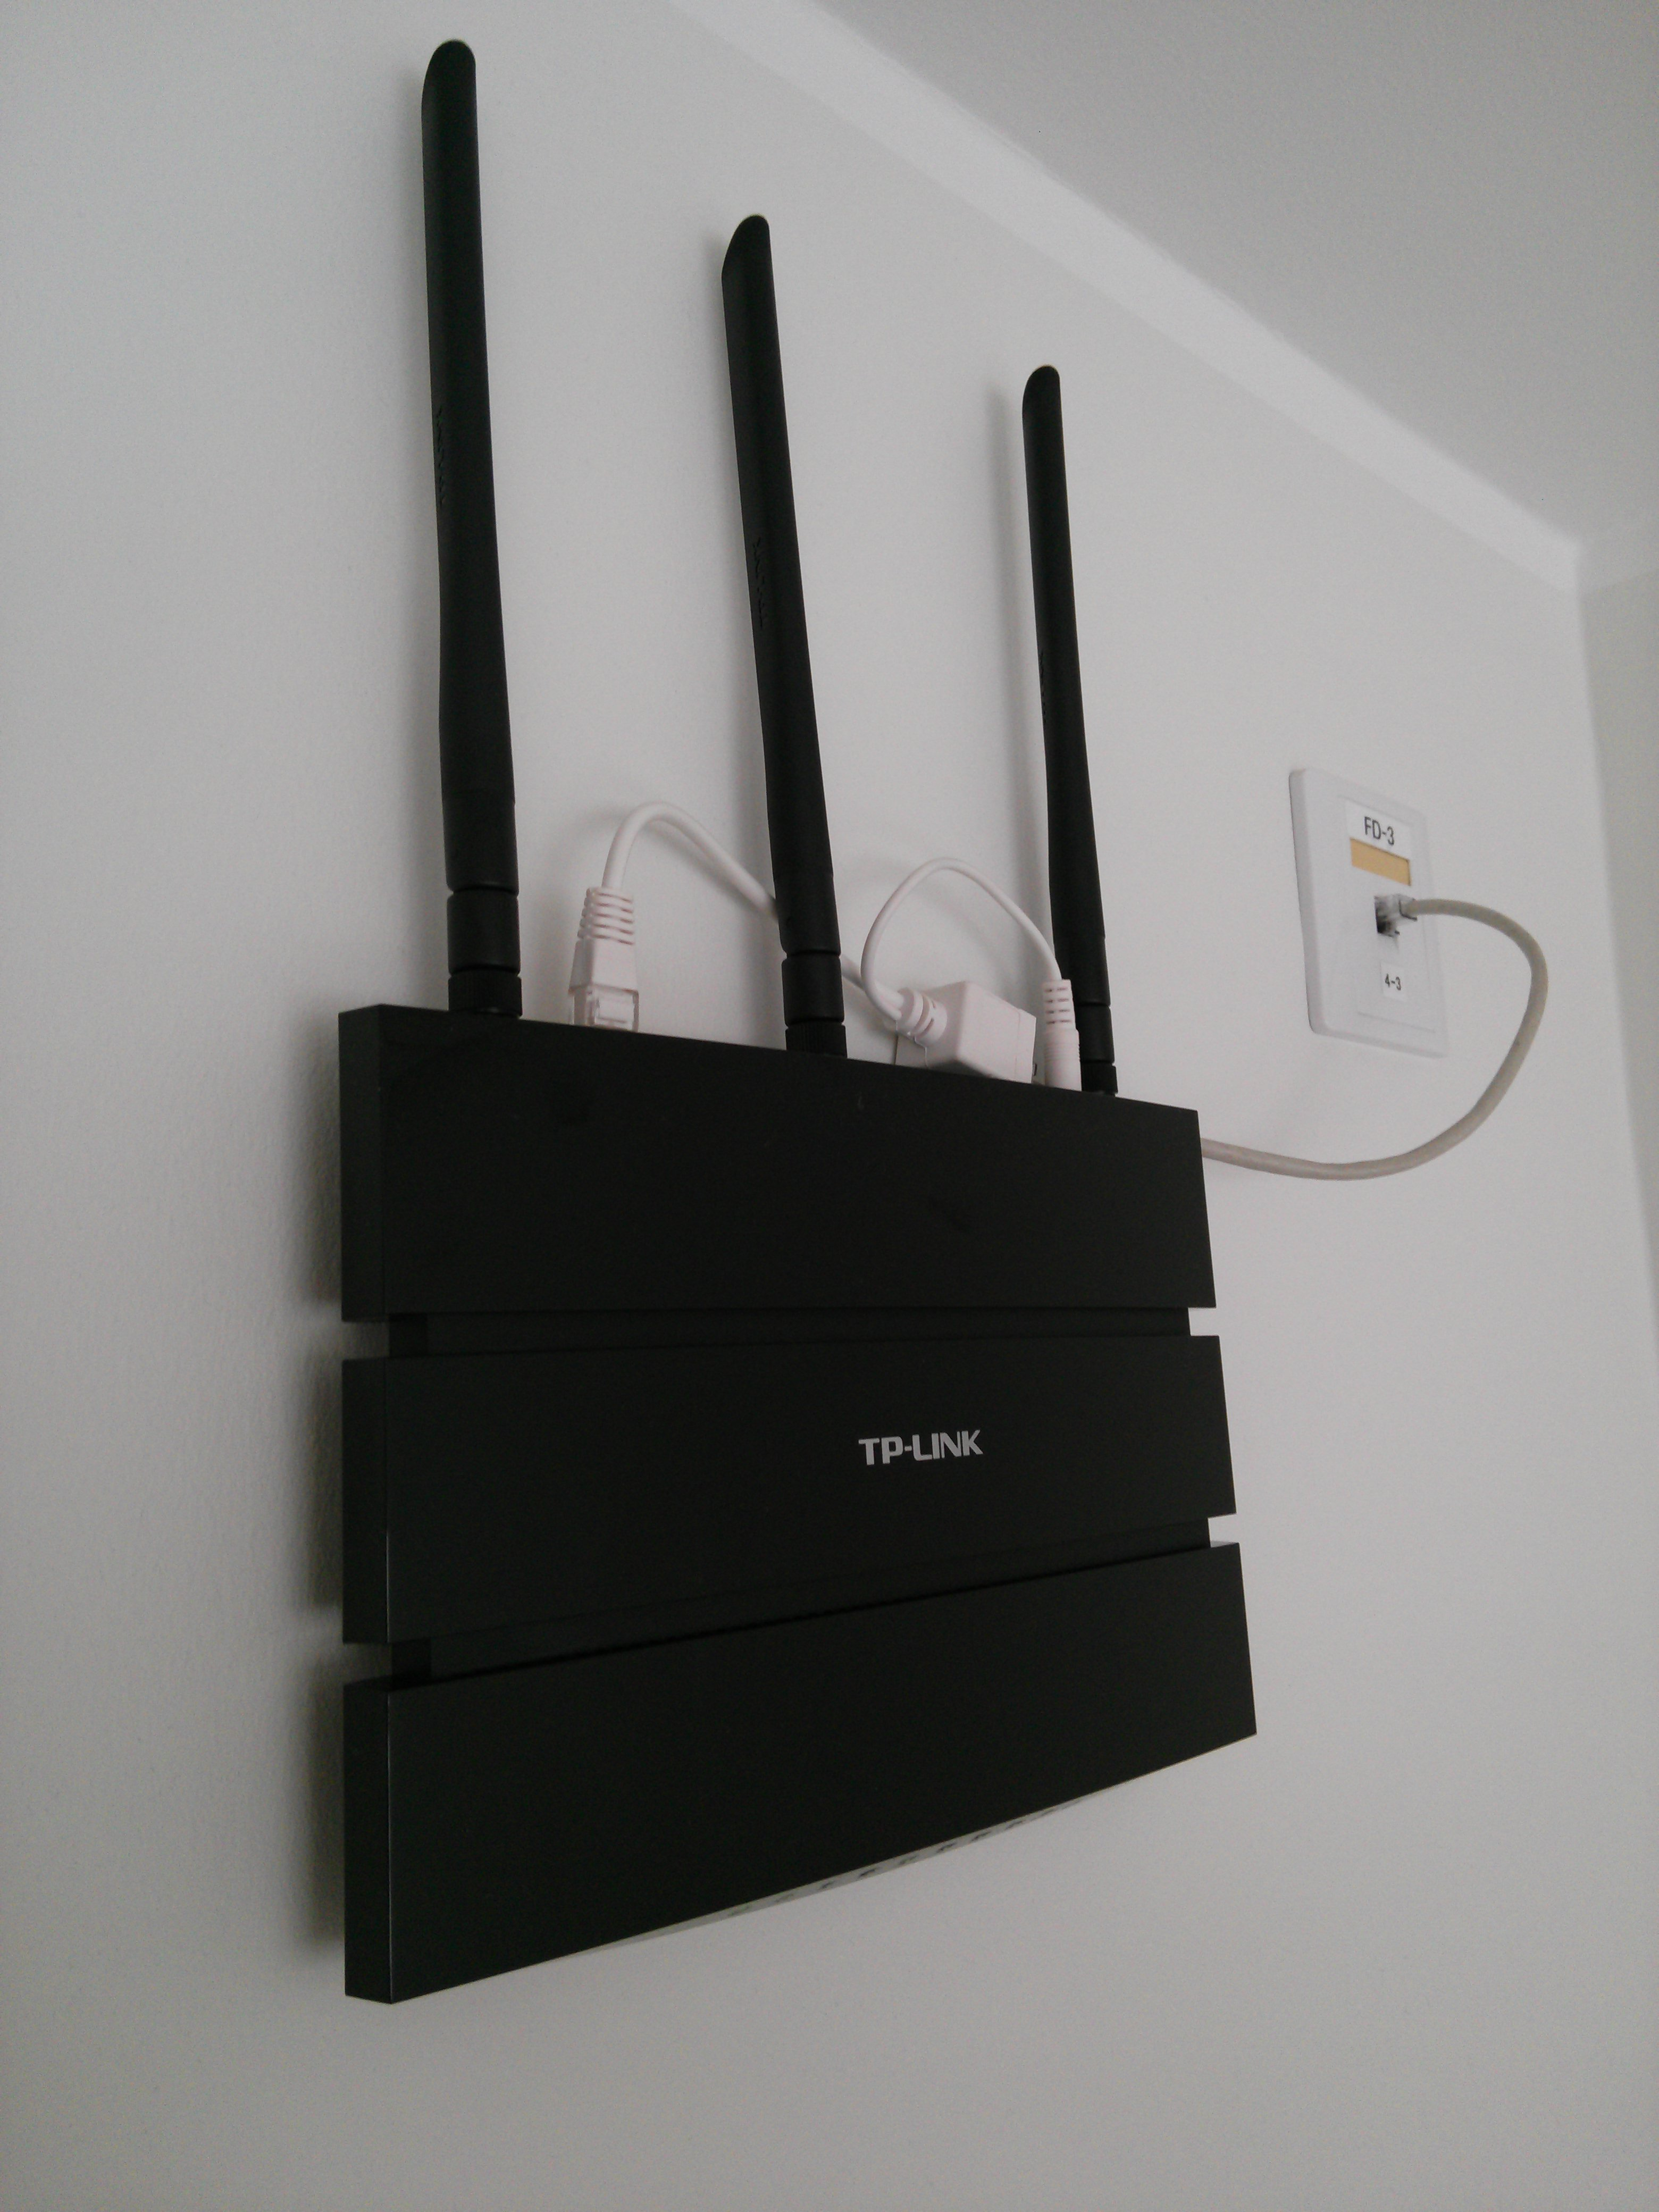
\includegraphics[scale=0.20]{img/haabneeme-wifi.jpg}}
\caption{TP-Link WDR4300 deployed with PoE injector}
\label{fig:digraph}
\end{figure}




\section{Conclusion}



\bibliographystyle{plain}
\bibliography{references}

\end{document}
